
\documentclass[a4paper,10pt,parskip=half]{scrbook}

\usepackage[usenames,dvipsnames]{xcolor}
\usepackage{graphicx}
\usepackage[utf8]{inputenc} %-- pour utiliser des accents en français
\usepackage{mathpazo}
\usepackage{amsmath,amssymb,amsthm} 
\usepackage[round]{natbib}
\usepackage{url}
\usepackage{xspace}
% \usepackage[left=20mm,top=20mm]{geometry}
\usepackage{geometry}
\usepackage[ruled,vlined,linesnumbered]{algorithm2e}
\usepackage{subcaption}
\usepackage{booktabs}
\usepackage{colortbl}
\usepackage{hyperref}
\usepackage{lastpage}
\usepackage{todonotes}
\usepackage{fontawesome}
\usepackage{ccicons}
\usepackage{gensymb}
\usepackage{tikz}
\usepackage[tikz]{mdframed}


\newcommand{\ie}{ie}
\newcommand{\eg}{eg}
\newcommand{\reffig}[1]{Figure~\ref{#1}}
\newcommand{\refsec}[1]{Section~\ref{#1}}


\setcapindent{1em} %-- for captions of Figures
\setcounter{tocdepth}{\sectiontocdepth}


% \renewcommand{\refname}{References \& further reading}
\renewcommand{\contentsname}{\vspace{-15mm}}

\definecolor{light-gray}{gray}{0.97}
\definecolor{myred}{RGB}{111,12,31}
\definecolor{mygreen}{RGB}{35,138,35}

\newmdenv[%
  outerlinewidth=1.5,%
  roundcorner=5pt,%
  linecolor=myred,%
  backgroundcolor=light-gray,%
  frametitle=\faExternalLink\ To read or watch,
]{link-box}

\newmdenv[%
  outerlinewidth=1.5,%
  roundcorner=5pt,%
  linecolor=mygreen,%
  backgroundcolor=light-gray,%
  frametitle=\faCog\ How does work in practice?,
]{practice-box}


\subject{An open access book}
\title{Computational modelling of terrains}
\author{Hugo Ledoux, Ken Arroyo Ohori, Ravi Peters}

\date{\today}

\begin{document}

%-------------------------------------------
\frontmatter
\maketitle
\tableofcontents
% \listoffigures
% \listoftables


%-------------------------------------------
\mainmatter

%!TEX root = ../terrainbook.tex

\setchapterpreamble[u]{\margintoc}
\chapter{What is a terrain?}%
\label{chap:whatisterrain}
\labch{whatisterrain}

\graphicspath{{whatisterrain/}}

%%%%%%%%%%%%%%%%%%%%%%%%%%%%%%%%%%%%%%%%%%%%%%%%%%%
% DTM == representation of the Earth's surface
% Dimensionality of DTM (2D, 2.5D, 2.75D, 3D)
% DTM, DSM, DEM
% nDSM: https://www.stadtentwicklung.berlin.de/umwelt/umweltatlas/ed610_03.htm
% Representation of DTMs in computers
%   - a DTM is a 2D field (object vs field discussion from GEO1002)
%   - 6 common representations: regularly spaced sample points; irregularly spaced sample points; contour lines; rectangular cells (raster); triangulated irregular networks (TIN); planar partition with arbitrary polygons.
%   - some are incomplete
%   - discussion data model vs data structure?




% \begin{center}
%   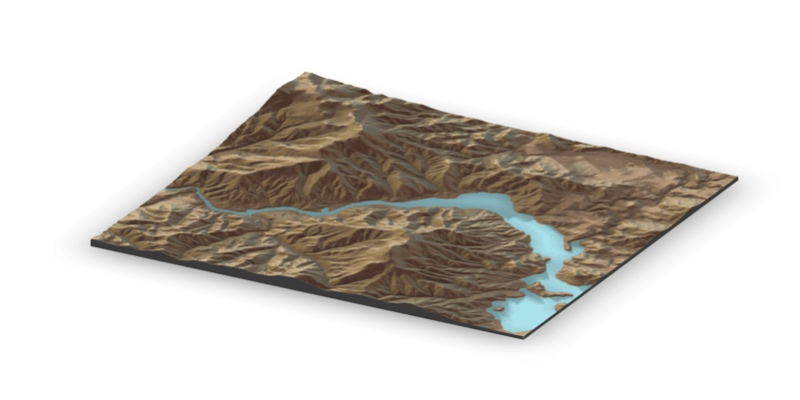
\includegraphics[width=0.95\linewidth]{figs/header.jpg}
% \end{center}


Defining what a terrain, also called a \emph{digital terrain model} (DTM), is not simple because there is no universal agreement, neither among practitioners nor in the scientific literature.
Different terms are used, often interchangeably.

In most cases, we can state that:

\begin{quote}
A terrain is a representation of the Earth's surface. 
It gives us the \emph{elevation}, which is the height above/below a certain reference point (a vertical datum)
\end{quote}

However, the ``Earth's surface'' is also not a clear concept, since several objects on it can be present, \eg\ man-made structures like buildings, roads, power lines, and bridges, and other objects like trees.

\begin{marginfigure}
  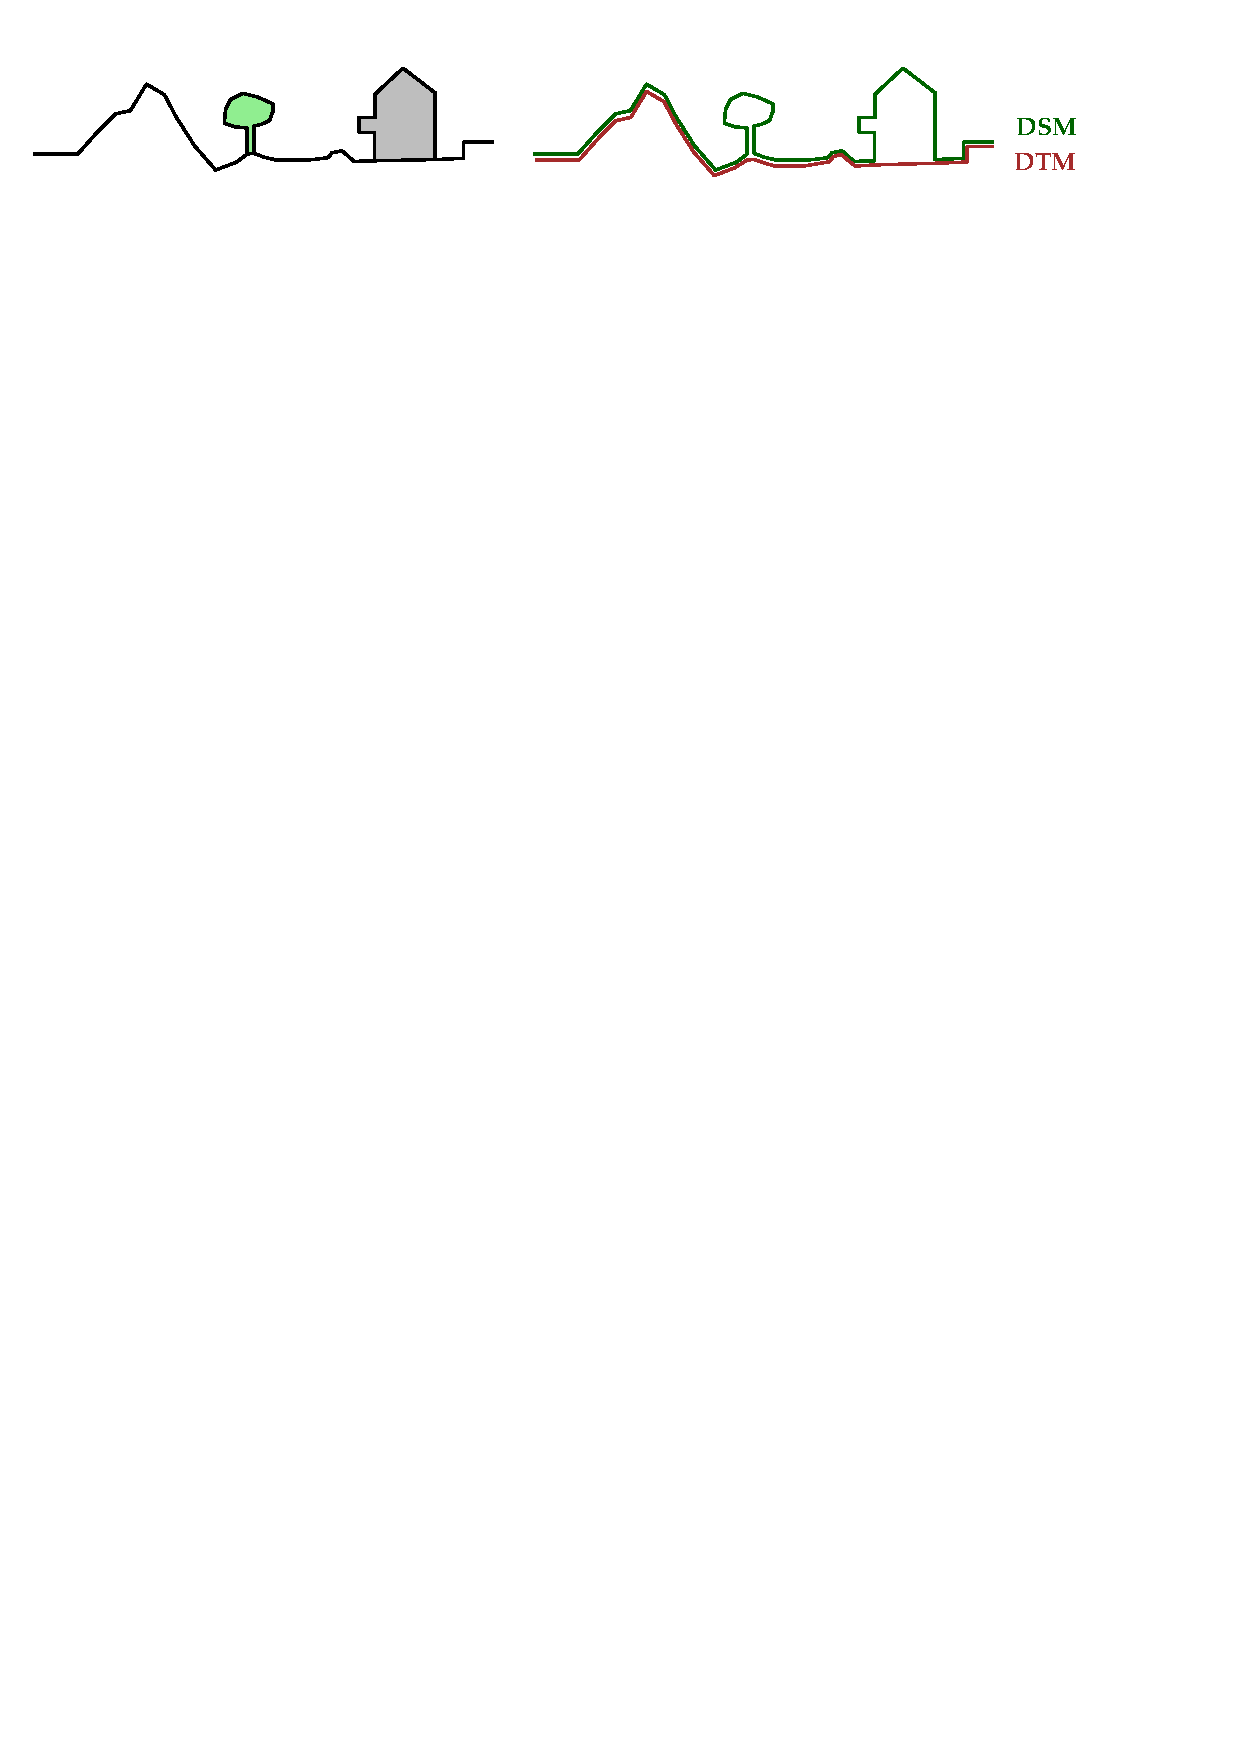
\includegraphics{figs/dtmdsm}
  \caption{\textbf{Top}: a terrain with a mountain, a tree, and a building. \textbf{Bottom}: its DSM and DTM.}%
\labfig{fig:dtmdsm}
\end{marginfigure}
We use the following definitions in this course (see \reffig{fig:dtmdsm}):
\begin{description}
  \item[DEM] (\textbf{D}igital \textbf{E}levation \textbf{M}odel). In the literal meaning of the term, it is simply a model of the elevation. A DEM is either a DSM or a DTM\@. 
  \item[DTM] (\textbf{D}igital \textbf{T}errain \textbf{M}odel). The surface of the Earth is the \emph{bare-earth}, that is no man-made objects or vegetation is present. 
  \item[DSM] (\textbf{D}igital \textbf{S}urface \textbf{M}odel). The surface includes all objects and structures on the terrain.
\end{description}

It should be noticed that in some countries a DEM is often synonymous with a grid of elevation (see below).


%%%
%
\section{Dimensionality of DTMs}

The term ``3D'' is misleading in a DTM context, as it is in a GIS context, because it might refer to three different concepts: 2.5D, 2.75D, and 3D (see \reffig{fig:dimgis}).
\begin{figure}[b]
  \centering
  \begin{subfigure}[b]{0.45\linewidth}
    \centering
    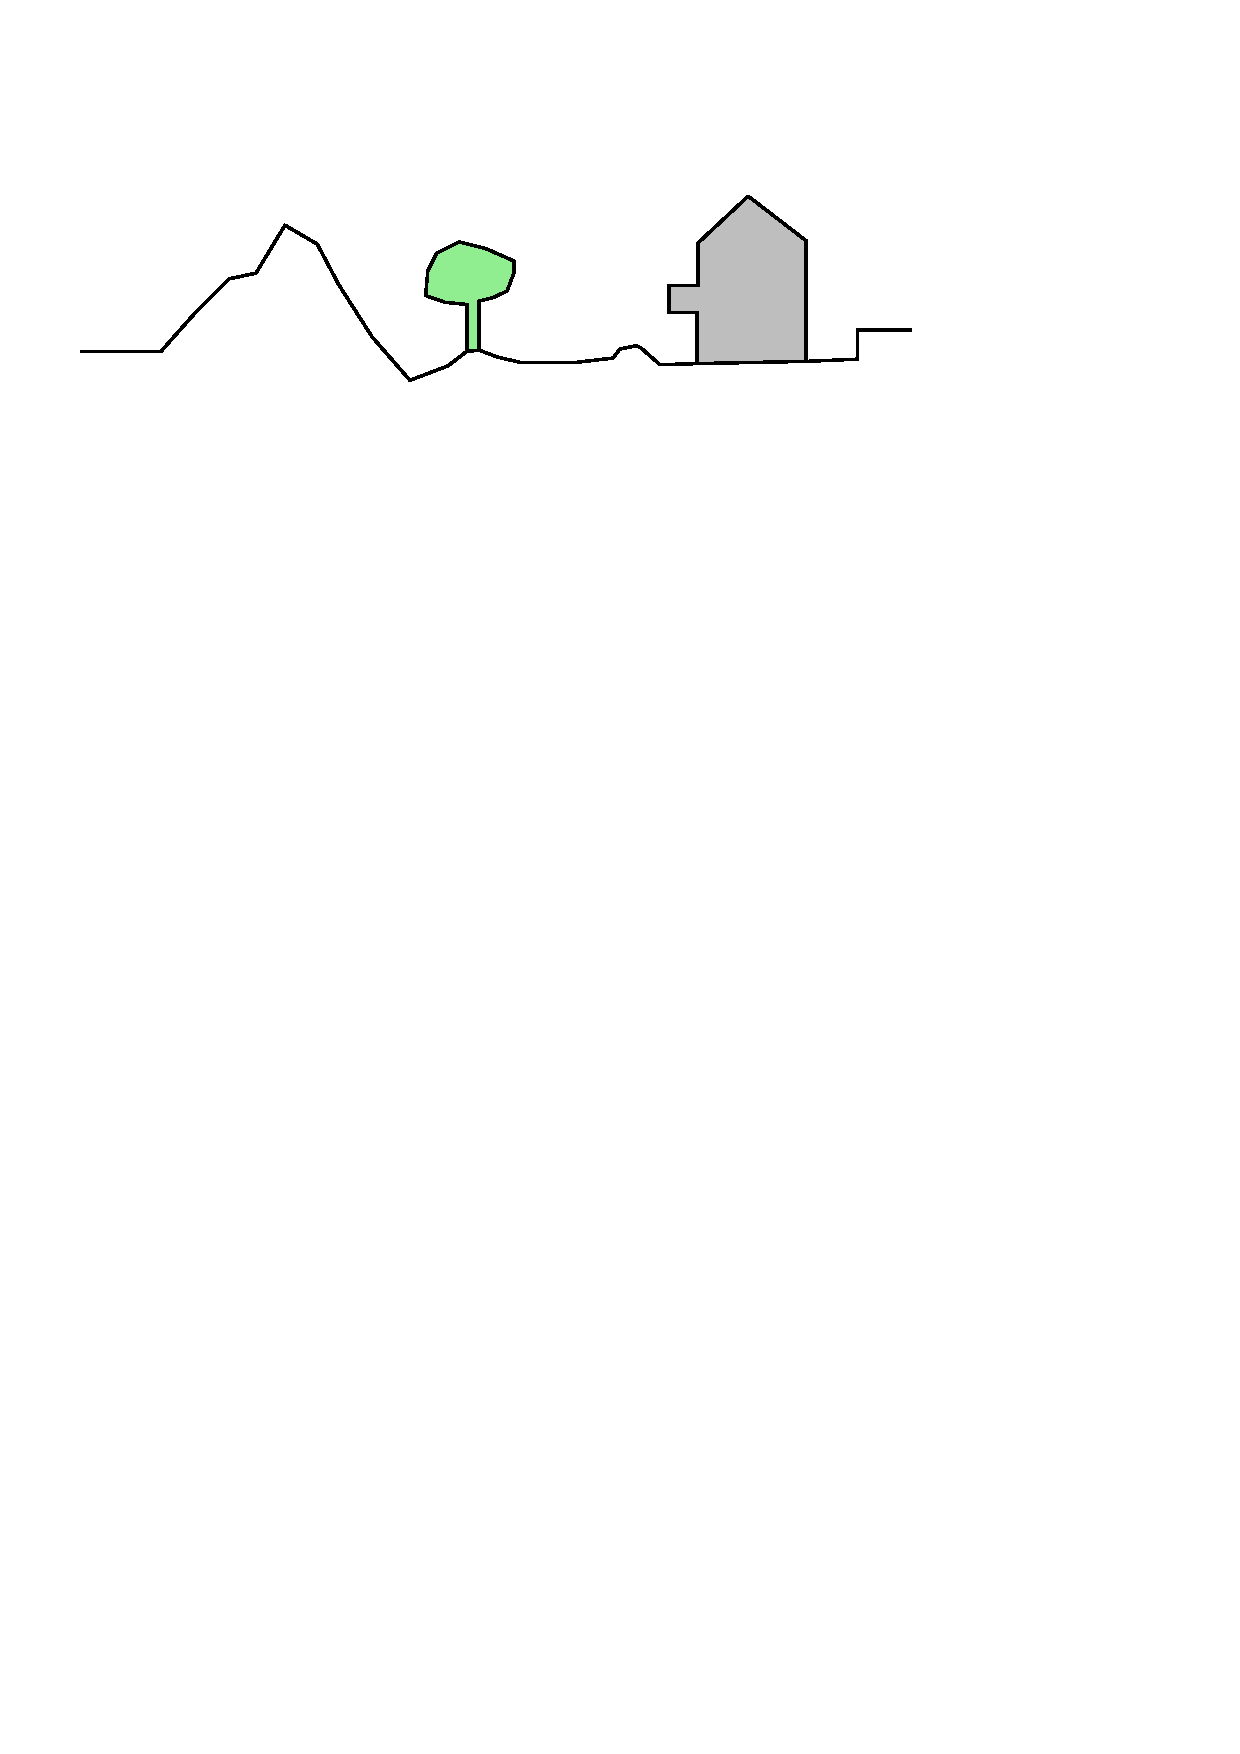
\includegraphics[page=1,width=\linewidth]{figs/dimgis}
    \caption{A terrain}\labfig{fig:dimgis:1}
  \end{subfigure}%
  \qquad %-- that adds some space between th 2 figures
  \begin{subfigure}[b]{0.45\linewidth}
    \centering
    \includegraphics[page=6,width=\linewidth]{figs/dimgis}
    \caption{2.5D modelling}\labfig{fig:dimgis:25}
  \end{subfigure}%
  \qquad %-- that adds some space between th 2 figures
  \begin{subfigure}[b]{0.45\linewidth}
    \centering
    \includegraphics[page=5,width=\linewidth]{figs/dimgis}
    \caption{2.75D modelling}\labfig{fig:dimgis:275}
  \end{subfigure}%
  \qquad %-- that adds some space between th 2 figures
  \begin{subfigure}[b]{0.45\linewidth}
    \centering
    \includegraphics[page=4,width=\linewidth]{figs/dimgis}
    \caption{Volumetric modelling, or full 3D}\labfig{fig:dimgis:3}
  \end{subfigure}%
  \caption{Different meanings for `3D GIS' in the context of terrains.}
\labfig{fig:dimgis}
\end{figure}


\subsection{2.5D} 
\labsec{ddd}
What is usually used for modelling terrains: a surface (which is a topologically a 2D object; also called a 2-manifold) is embedded in 3D space, and each location ($x,y$) is assigned to one and only one height $z$.
% \marginnote{Text of the note}
In other words, the surface can be projected to the $xy$-plane and maintain its topology.
When we refer to terrains in this course, this is what is usually mean, unlike explicitly stated otherwise.
This is often what is used in GIS software, and both the well-known raster/grid  is such a case.
Observe that this restricts the real-world cases that can be modelled because, as shown in \reffig{fig:dimgis}b, vertical surfaces (\eg\ walls of a building if we model all man-made objects with the terrain to construct a digital surface model), overfolds (\eg\ the balcony of a house) and caves are impossible to represent.
As shown in the figure, these are modelled as nearly vertical surfaces; in practice the wall of building could deviate by for instance 1 degree from the vertical. 

\subsection{2.75D} 
This also refers to a surface (a 2-manifold) but unlike for the 2.5D case, the surface is not restricted to be projectable to the 2D plane (see \reffig{fig:dimgis}c).
Thus, more than one $z$ value is allowed for a given location ($x,y$).
The term '2.75D' was coined because: it is more than 2.5D, but less than 3D.
The surface represents the exterior of all objects/features together, and vertical walls are allowed.
Surface modelling is popular in CAD, but in the GIS it is rather rare.
We are not aware of any popular GIS software that allows us to model a terrain as a 2.75D and perform operations on it.

\subsection{Full 3D, or volumetric modelling} 
This refers to the modelling of not only the boundaries of objects, but also of the interior of these.
Notice for instance in \reffig{fig:dimgis}d that each building is represented with a solid.
The volume of buildings can therefore be calculated (since the ground floor of buildings would be modelled for instance), while with the other variations it is not possible. 
Such a representation is usually done with a 2.5D terrain (although a 2.75D could also be used) and a set of buildings/objects that are connected to the terrain.



%%%
%
\section{2.5D terrain == field}
\index{field}

In the context of this course, we assume that a terrain is a 2.5D object, and therefore a terrain can be considered as a \emph{field}.
A field is a model of the spatial variation of an attribute $a$ over a spatial domain, which in our case is $\mathbb{R}^2$, the two-dimensional Euclidean space.
It is modelled by a function mapping one point $p$ in $\mathbb{R}^2$ to the value of $a$, thus 
\[
  a = f(p)
\]
The function can theoretically have any number of independent variables, but in the context of a terrain the function is usually bivariate ($x,y$).

%

The representation of a field in a computer faces many problems. 
First, fields are continuous functions, and, by contrast, computers are discrete machines. 
Fields must therefore be \emph{discretised}, \ie\ broken into finite parts.
\index{discretisation}
Second, in practice it is usually impossible to measure continuous phenomena everywhere, and we have to resort to collecting samples at some finite locations and reconstructing fields from these samples.
The discretisation task therefore begins at the acquisition phase, and is affected by the acquisition tools and techniques (more about this in \refchap{chap:acquisition}).
This fact is aggravated for fields as found in GIS-related disciplines because, unlike disciplines like medicine or engineering, we seldom have direct and easy access to the whole object of interest.


%%%
\subsection{What is needed to represent a field/terrain?}

To represent a terrain in a computer, and be able to manipulate it (\ie\ edit the terrain and extract information such as slope), two things are needed:
\begin{enumerate}
  \item a set of samples that were collected to study the terrain, for instance a point cloud obtained from airbone laserscanning or photogrammetry (see \refchap{chap:acquisition} for details).
  \item a set of rules to obtain one and only one elevation value at any location ($x,y$); in other words, to reconstruct the continuity of the surface from the discrete samples.
  This operation is referred to as spatial interpolation (Chapters~\ref{chap:interpol} and~\ref{chap:kriging}). 
\end{enumerate}


%%%
\subsection{Strategy \#1: points + global interpolation function.}
This means storing the original sample points with the parameters of the \emph{global} spatial interpolation method that is best suited to the distribution of the samples and their accuracy.
Global methods are for instance inverse-distance to a power, natural neighbours, or Kriging.
This strategy is used because one can compactly represent a field (only the samples and a few parameters need to be stored).

Notice that this strategy permits us to reconstruct the continuity of a terrain from the samples by calculating the value of the elevation, but that this value is \emph{not} persistently stored in memory.
It is therefore less used in practice than the next strategy, which allows us to permanently store the terrain in a file and avoids us recomputing every time al the needed elevation values.


%%%
\subsection{Strategy \#2: piecewise spatial models}
This means that the spatial interpolation function used is \emph{piecewise} (instead of being global).
\marginnote{piecewise function}
\index{piecewise function}
That is, the two-dimensional domain of the terrain (the $xy$-plane) is tessellated, or partitioned, into several pieces, and for each of these we assign an interpolation function describing the spatial variation in its interior.
This function is usually a simple mathematical function:
\begin{itemize}
  \item constant function: the value of the modelled attribute is constant within one cell;
  \item linear function;
  \item higher-order function.
\end{itemize}

%

In general, we  classify the tessellations of space into three categories (as shown in \reffig{fig:tesstypes}): \emph{regular}, \emph{irregular}, and \emph{hierarchical}.
\begin{marginfigure}
  \centering
  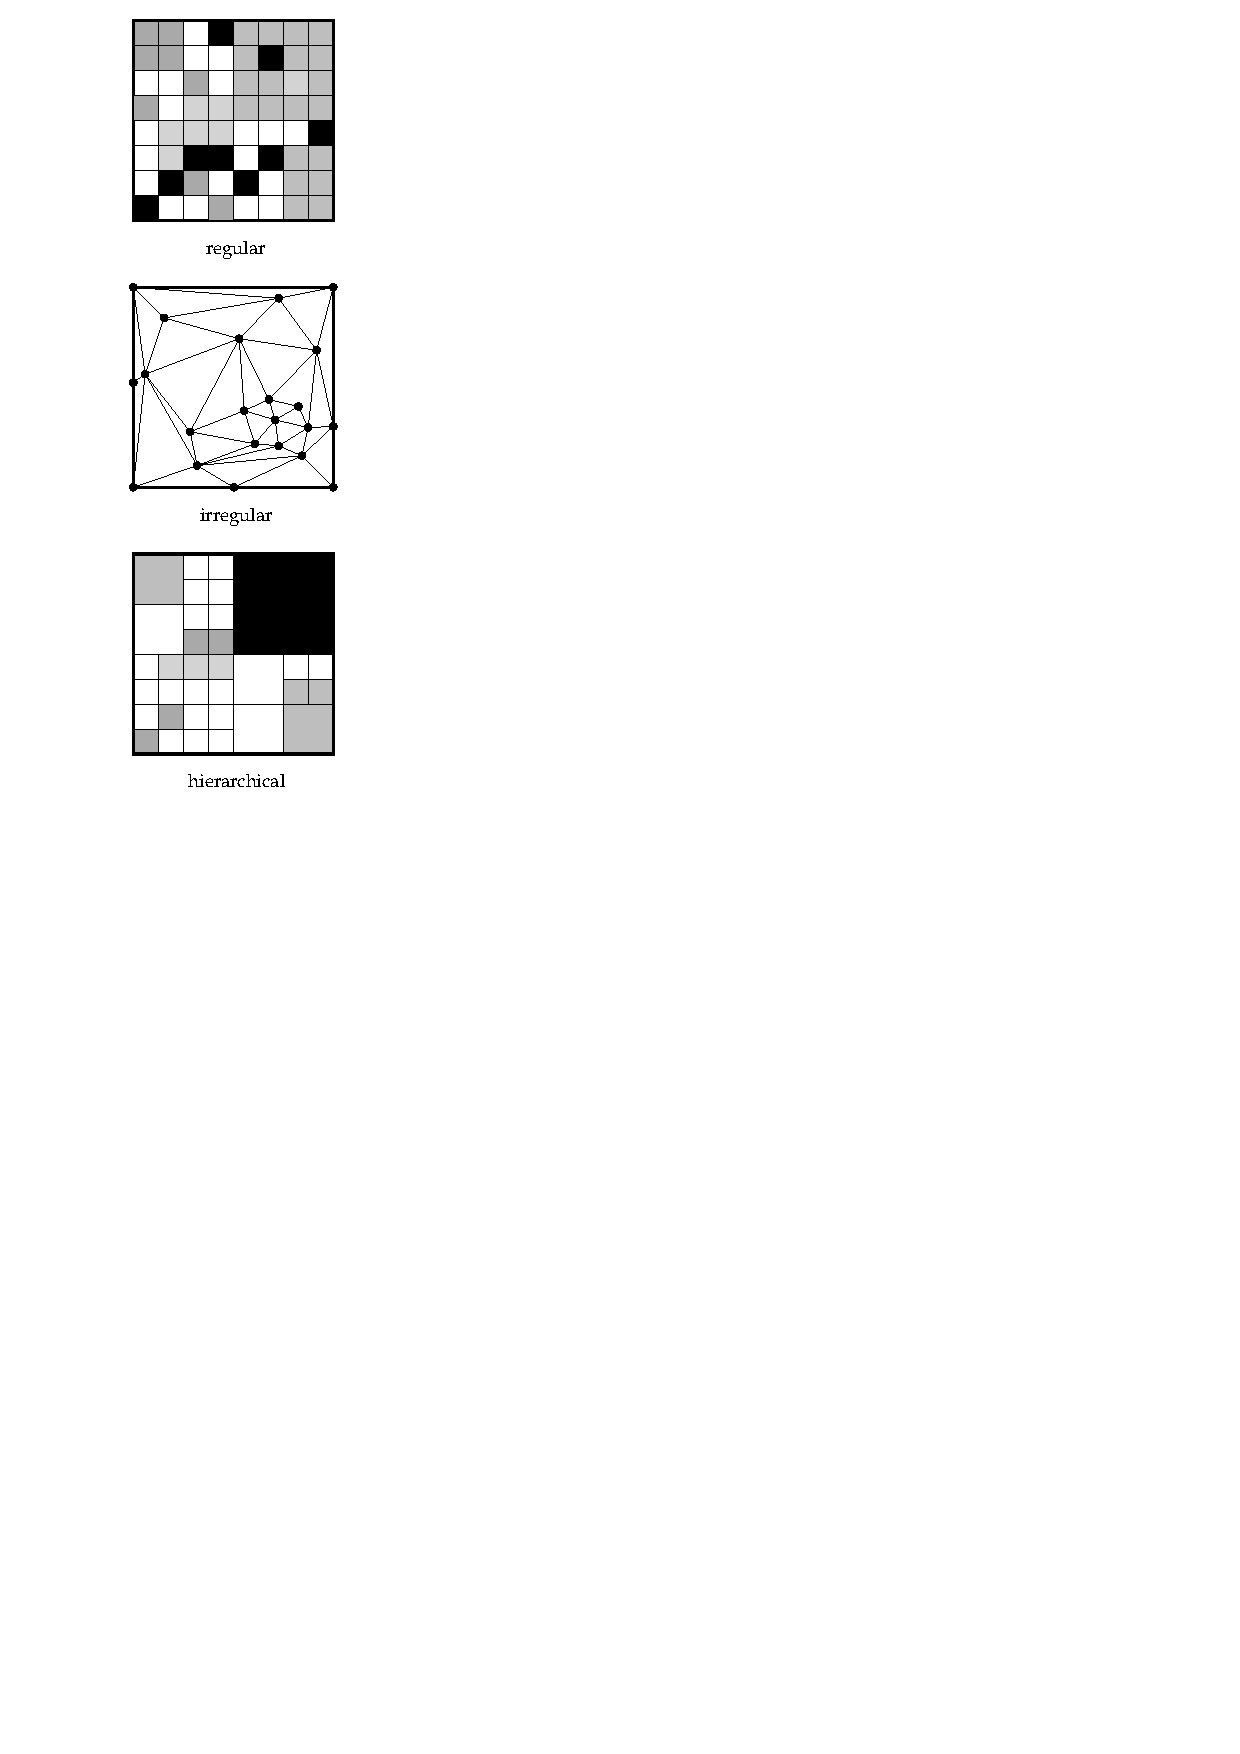
\includegraphics[width=0.7\textwidth]{figs/tesstype}
  \caption{Type of tessellations.}% 
\labfig{fig:tesstypes}
\end{marginfigure}

%

Piecewise models typically imply that a supporting data structure is constructed, and stored, to represent the tessellation.
% (it is however possible to construct on-the-fly some well-known structures only when they are needed since they have formal rules).
Some of these tessellations partition arbitrarily the space, while some are based on the spatial distribution of the sample points.


%%%
%
\section[Data models for terrains]{Data models for representing terrains in a computer}

\subsection{Spatial data models $\neq$ data structures}

In the GIS literature, there exists a confusion between the terms ``spatial model'' and ``data structure''. 
The confusion originates from the fact that object and field views of space are usually implemented in a GIS with respectively vector and raster models. 
However, this is not always the case as TINs can be used for fields for instance.
A ``spatial data model'' offers an \emph{abstract} view of a data structure, it is an abstraction of the reality.
A data structure is the specific implementation of a spatial data model, and deals with storage, which topological relationships are explicitly stored, performance, etc.
The same spatial data model can therefore be implemented with different data structures.



%%%
\subsection{Regular Tessellations} 

As shown in \reffig{fig:tesstypes}a, all the cells have the same shape and size.
The most common regular tessellation in GIS and in terrain modelling is by far the grid (or raster representation), in which the cells are squares in 2D (usually called \emph{pixels}, a portmanteau of `picture' and `element', as an analogy to digital images).
However, while they are not common in practice, other regular shapes are possible, such as hexagons or triangles.

%

Observe that a regular tessellation often arbitrarily tessellates the space covered by the field without taking into consideration the objects embedded in it (the samples). 
This is in contrast with irregular tessellations in which, most of the time, the shape of the cells constructed depends on the samples.

In practice this means that, if we have a terrain stored as a regular tessellation we can assume that it was constructed from a set of samples by using spatial interpolation.
Converting sample points to cells is not optimal because the original samples, which could be meaningful points such as the summits, valleys or ridges of a terrain, are not necessarily present in the resulting tessellation. 
There is a loss of information, since the exact location of the meaningful points are lost.
% Also, when a practitioner has access to a grid, she often does not know how it was constructed and what interpolation method was used, unless meta-data are available.

%

\paragraph{Concrete example: a 2D grid.}
A 2D grid, stored for instance with the GeoTIFF format, is thus a piecewise representation of a 2D field: a regular tessellation where each cell has a constant function.
The value assigned to each cell is an estimation previously obtained by spatial interpolation.
However, for a given grid, it is usually unclear if the value of a cell is for its centre, or for one of its vertices (and if it is the case, for which one?).
Different formats have different rules, and converting a field represented with one format to another one (while retaining the same cell resolution and spatial extent) can shift the value from the centre to the top-left corner for instance.

%

The wide popularity of regular tessellations in terrain modelling is probably due to simplicity and to the fact that they permit us to easily integrate 2D remote sensing images and terrains.
Indeed, a grid is naturally stored in a computer as an array (each cell is addressed by its position in the array, and only the value of the cell is stored), and thus the spatial relationships between cells are implicit. 
This is true for any dimensions, thus, contrary to other tessellations, grids are very easy to generalise to higher dimensions.
The algorithms to analyse and manipulate (Boolean operations such as intersection or union) are also straightforwardly implemented in a computer. 

On the other hand, grids also suffer problems.
First, the size of a grid can become massive for data at a fine resolution; this problem gets worse in higher dimensions.
Second, grids scale badly and are not rotationally invariant, \ie\ if the coordinate reference system used is changed, then the grid needs to be reconstructed to obtain regular cells whose boundaries are parallel to the axes of the reference system.
To assign a new value to the transformed cells, spatial interpolation is needed, which is often performed not by re-using the original samples, but by using the values of the neighbouring cells.
Unfortunately, each time a grid is transformed its information is degraded because not the original samples are used, but interpolated values.



%%%
\subsection{Irregular Tessellations} 

The cells of an irregular tessellation can be of any shape and size, and they usually `follow'---or are constrained by---the samples points that were collected, albeit this is not a requirement. 
Subdividing the space based on the samples has the main advantage of producing a tessellation that is \emph{adaptive} to the distribution of the samples. 
The subdivision is potentially better than that obtained with regular tessellations (which subdivide arbitrarily the space without any considerations for the samples).

%

The most known examples of the use of irregular tessellations in terrain modelling is the \emph{triangulated irregular network}, or TIN\@.
\index{TIN}

As shown in \reffig{fig:tin}, a TIN refers to an irregular tessellation of the $xy$-plane into non-overlapping triangles (whose vertices are formed by three sample points), and to the use of a linear interpolation function for each triangle. 
\begin{marginfigure}
  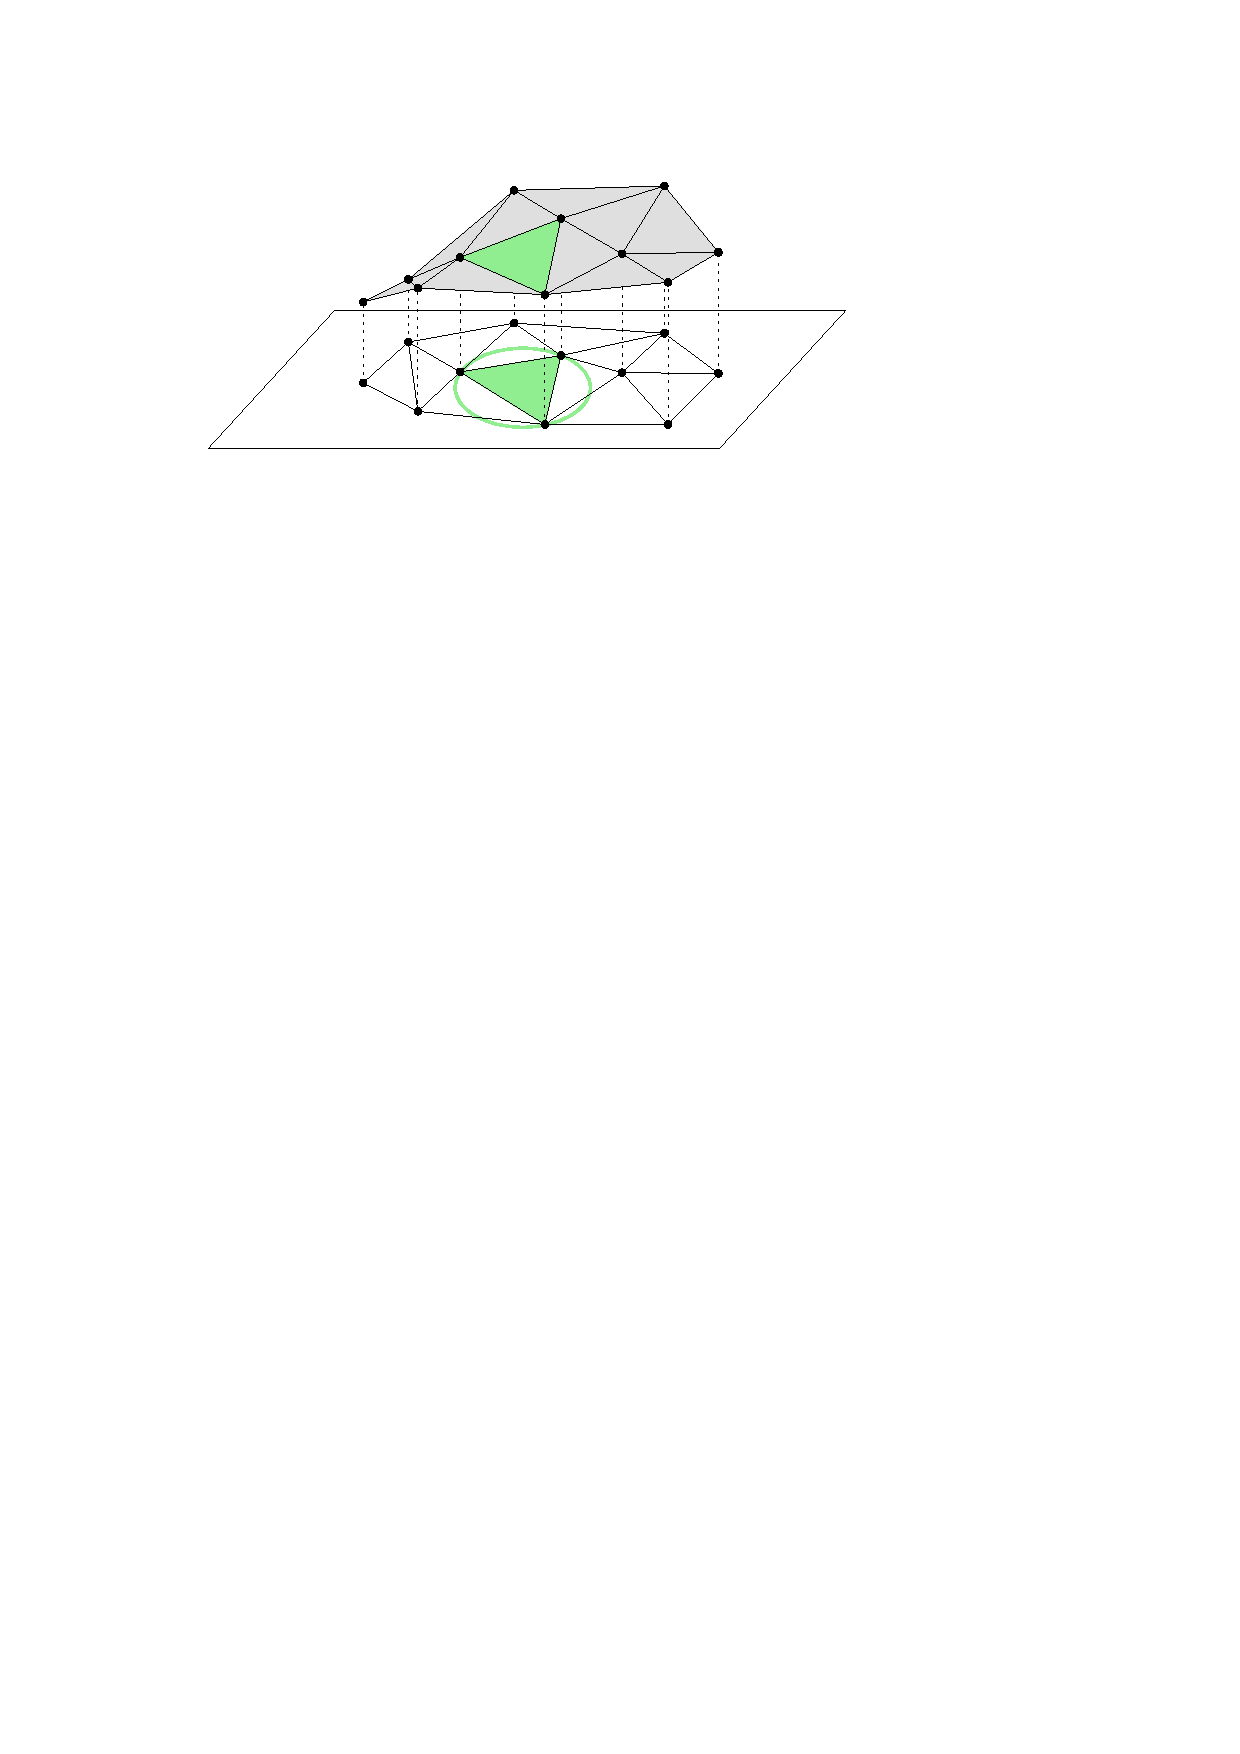
\includegraphics{figs/tin}
  \caption{A TIN is obtained by lifting the vertices to their elevation. All the triangles are usually Delaunay, \ie\ their circumcircle (green) is empty of any other points in the plane.}%
\labfig{fig:tin}
\end{marginfigure}
One way to explain the 2.5D properties of a TIN is as follows: if we project vertically to the $xy$-plane the triangles in 3D space forming the TIN, then no two triangles will intersect.

While not a requirement, the triangulation is usually a Delaunay triangulation (more about this in Chapter~\ref{chap:dtvd}).
The main reason is that Delaunay triangles are as ``fat'' as possible (long and skinny triangles are avoided), and thus they behave better for interpolation.
As can be seen in~\reffig{fig:whydt},
\begin{figure}
  \centering
  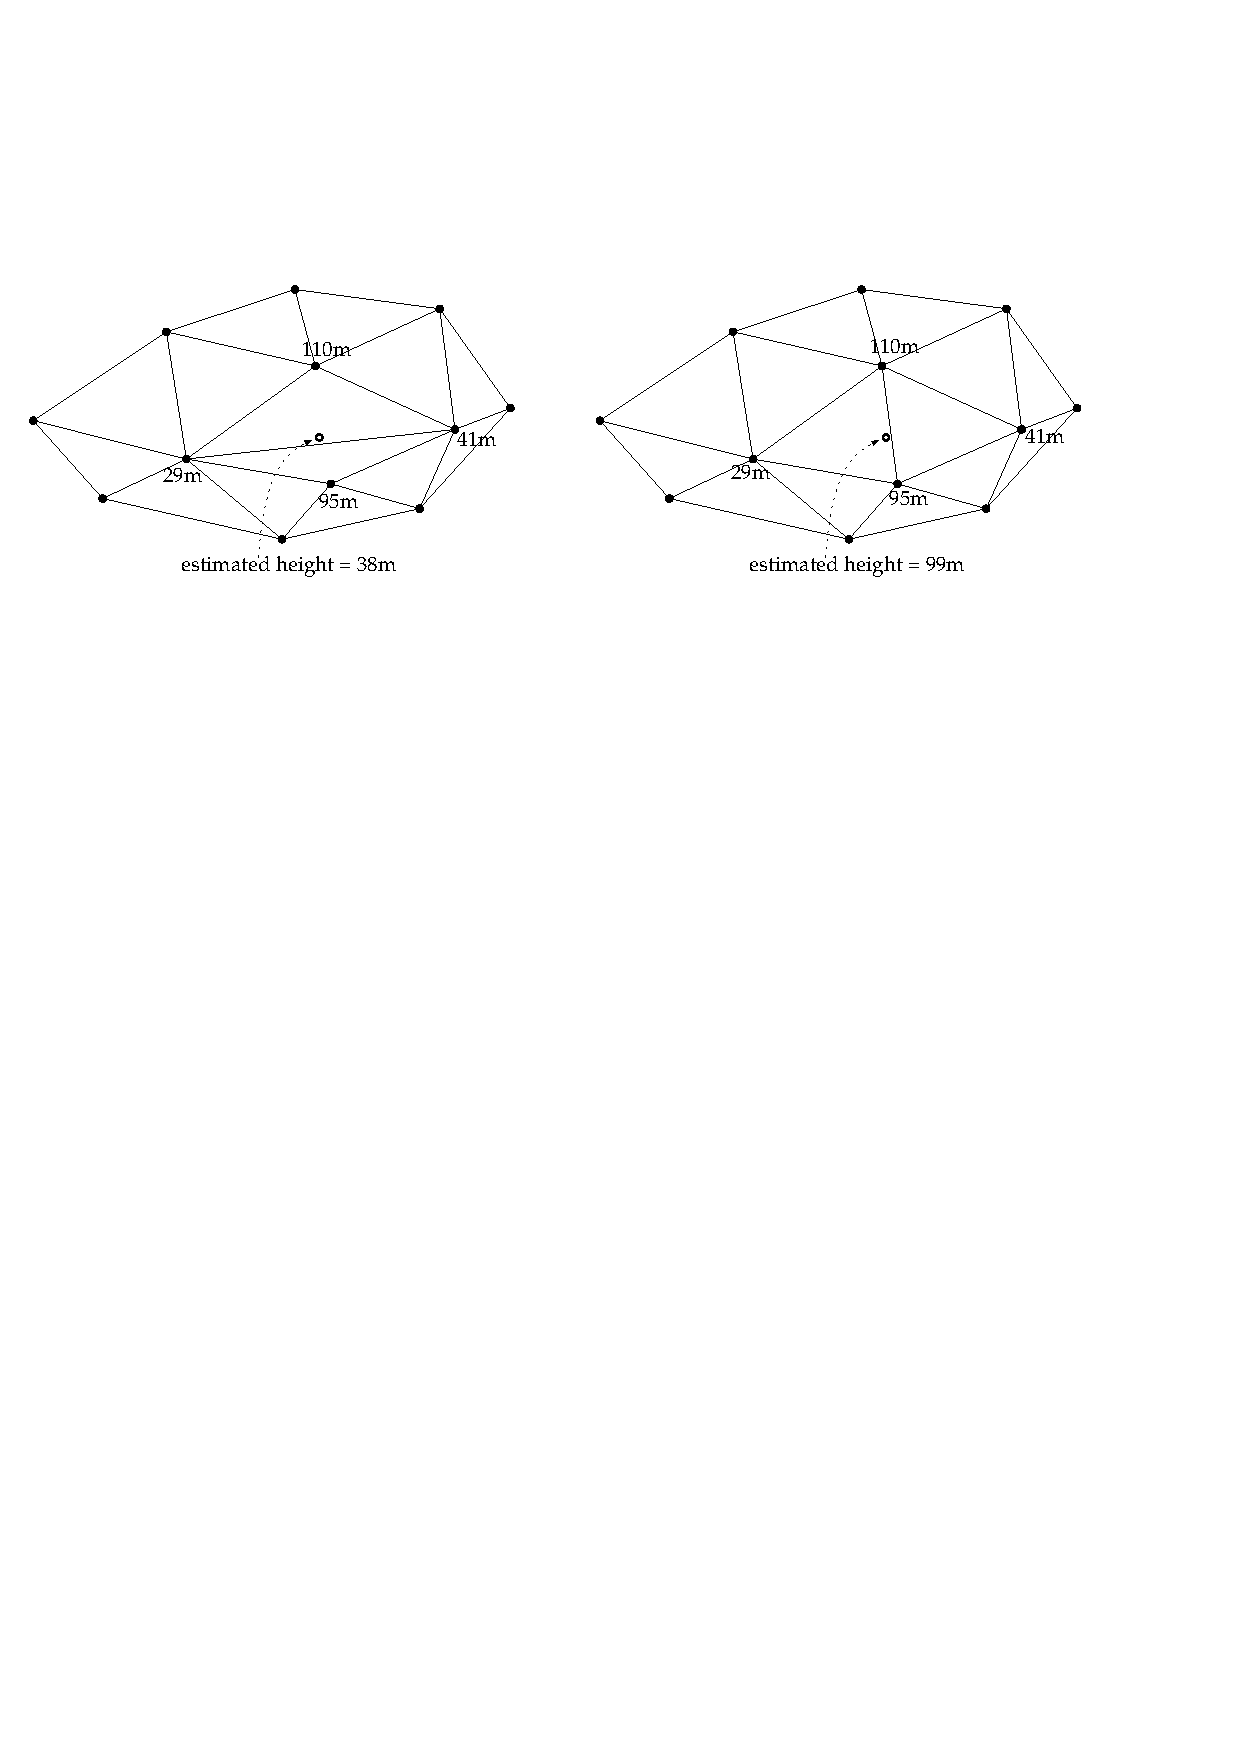
\includegraphics[width=\linewidth]{figs/whydt}
  \caption{Two TINs (left is a DT, right has one non-Delaunay edge) and the result of estimating with linear interpolation in the TIN\@.}%
\labfig{fig:whydt}
\end{figure}
the estimated value can be significantly different, and in this case the right one would make more sense since sample points that are closer to the interpolation location are used (in the TIN on the left, the value of 95m is not used).

%

Each of the points (which becomes vertices in the triangulation) are lifted to its elevation to create a surface, embedded in three dimensions, approximating the morphology of the terrain.
The value of elevation at an unsampled location $p$ is obtained by linearly interpolating on the plane passing through the three vertices of the triangle containing $p$. 
TINs are the most popular alternatives to 2D grids for modelling elevation; both representations have advantages and disadvantages.

%
 
A TIN in which a linear interpolation function is used yields a $C^0$ piecewise representation, \ie\ it is a continuous function but at the edges of the triangles the first derivative is not possible.
It is possible to use higher-order functions in each triangle of a TIN, to construct a $C^1$ or $C^2$ field, \ie\ where the first and second derivative of the surface can be obtained. 



%%%
\subsection{Hierarchical tessellations}

Hierarchical tessellations attempt to reduce the number of cells in a tessellation by merging the neighbouring cells having the same value (thus yielding cells of different sizes).
While both regular and irregular tessellations can be hierarchical, in the context of the representation of terrains, the former is more relevant and is sometimes used in practice.

% Irregular hierarchical tessellations, usually triangulations, are used for obtaining multi-resolution models, or act as a spatial index for efficiently accessing triangles.
% Their use as a support to construct a piecewise function is not necessary because irregular tessellations have cells of different sizes and shapes.
% Consequently, only hierarchical regular tessellations are discussed in the following.

%

A commonly used hierarchical structure in two dimensions is the \emph{quadtree}, which is a generic term for a family of tessellations that recursively subdivide the plane into four quadrants.
As is the case for grids, quadtrees are relatively easily implemented in a computer because they are trees in which each node has exactly four children, if any.

%

The shortcomings of regular hierarchical tessellations are similar to those of regular tessellations: the rotation and scaling operations are difficult to handle.
The main advantage of using them---saving memory space---is present only when there is spatial coherence between cells having the same attribute value, \ie\ when they are clustered together.
Indeed, the size of a quadtree is not dependent on the number of cells, but on their distribution.
The quadtree of a 2D grid having no two adjacent cells with the same value (\eg\ a checkers board) contains the same number of cells as the grid, and its size would most likely be worse because of the overhead to manage the tree.
Another disadvantage is that the notion of neighbours, which is straightforward in regular tessellations, is less trivial.


%%%
\subsection{Other common terrain representations used in GIS}

\begin{marginfigure}
  \centering
  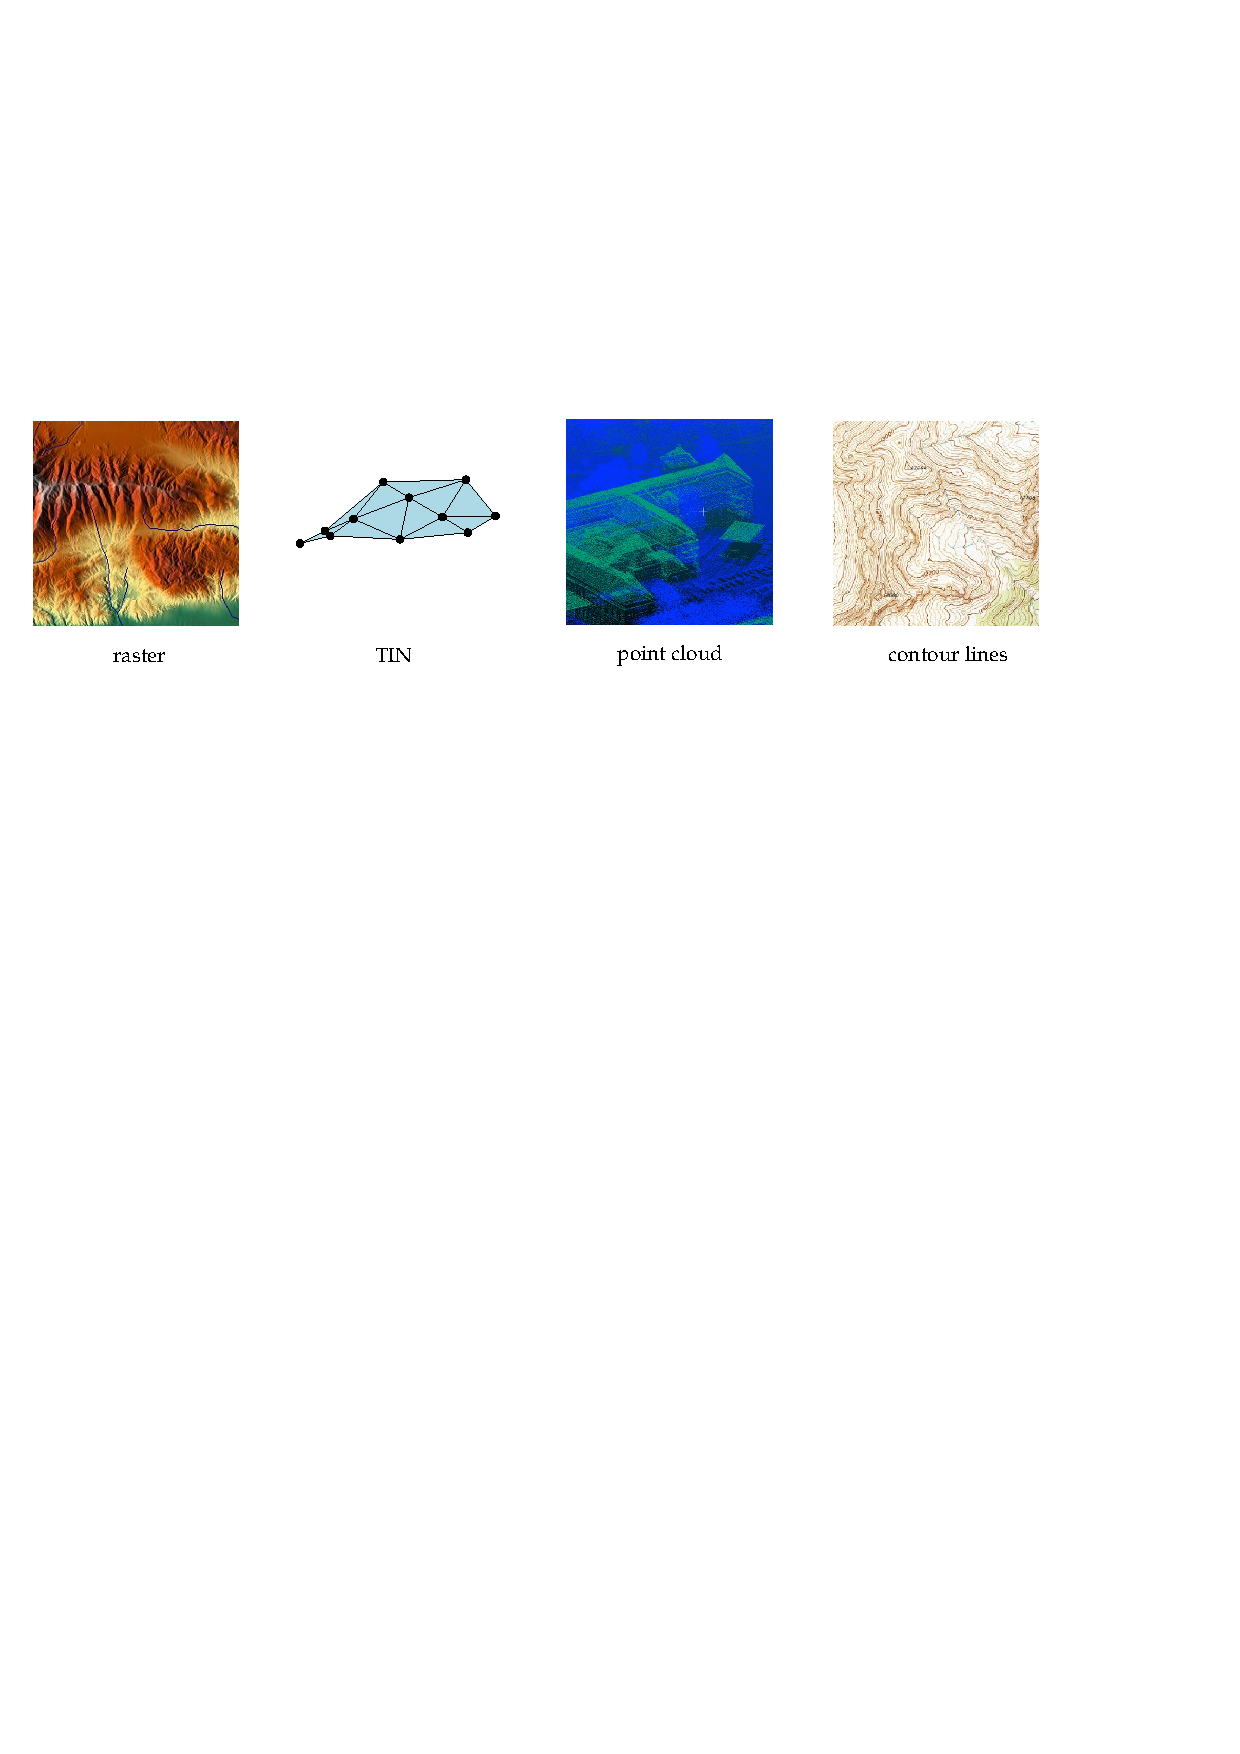
\includegraphics[width=0.75\linewidth]{figs/reps}
  \caption{Four most common data models for terrains.}%
\labfig{fig:reps}
\end{marginfigure}

In the GIS literature, besides the ones above, different representations for terrains are often listed, the two most relevant being:
\begin{enumerate}
  \item irregularly spaced sample points, such a point cloud; 
  \item contour lines.
\end{enumerate}
It should be noticed that these two are however \emph{incomplete}: the set of rules to reconstruct the surface at unsampled locations is not explicitly given, they are not continuous surfaces.
Conceptually speaking, these should therefore not be considered valid representations of a terrain.
While this might seems odd, this is in line with the consensus among practitioners today, where a point cloud or contour lines would typically be used as an input to a process to generate a terrain.

We will nevertheless consider these in the course; the four representations we will use are shown in \reffig{fig:reps}.

%

\paragraph{Contour lines.}

Given a bivariate field $f(x,y) = z$, an \emph{isoline} (commonly named contour line) is the set of points in space where $f(x,y) = z_0$, where $z_0$ is a constant. 
Isolines have been traditionally used to represent the elevation in topographic maps and the depth in bathymetric maps for navigation at sea. 

%

% TODO : change the nicked contour example jpg?
\begin{marginfigure}
  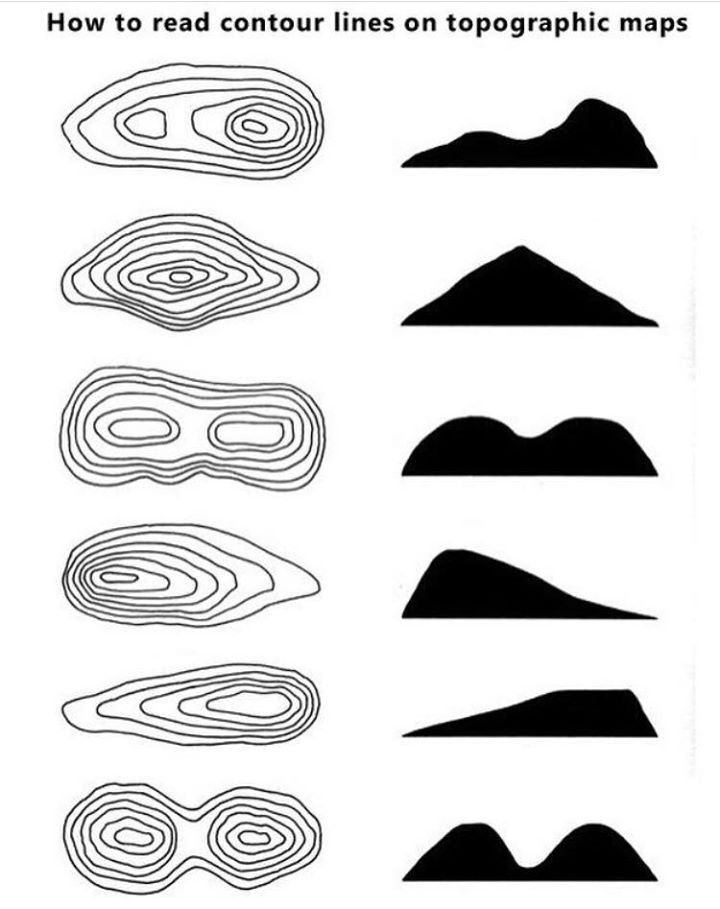
\includegraphics{figs/contours.jpg}
  \caption{A few examples of terrain features and their contour lines. (Figure from \url{https://linguagemgeografica.blogspot.com/})}%
\labfig{fig:contours}
\end{marginfigure}

One particular property of an isoline is that its direction is always perpendicular to the direction of the steepest slope of the terrain. 
Another property that follows from the $2.5D$ property of the field is that contours neither intersect themselves nor each other.

%

The purpose of isolines on a map is to reveal the shape of the underlying terrain. 
By observing the shape and interrelation of neighbouring contours, the presence and significance of surface features becomes apparent; see~\reffig{fig:contours} for a few examples.
It should be noticed that data between contours is absent in the contour map. 
Yet, in case of good contours the reader will still be able to deduct the general morphology of the field. 
It is even so that the use of contours will speed up the map reading process, as it conveys just that relevant bit of data to the map reader rather than `flooding' the reader with information which essentially makes the user do his own cartographic selection. 
Contouring is a form of discretizing the field that makes it easier to use a map. 
Naturally, this comes at a price. 
The level of approximation of the field can (dramatically) differ between contours, the biggest error would be midway in between contour lines. 
But, depending on the relation between the spacing between contours (the \emph{contour interval}) and the map scale, which in turn is dependent on the map application, this effect may be neglected.


%

In practice, isolines are only approximated from the computer representation of a field.
They are usually extracted directly from a TIN or a regular grid. 
As shown in~\reffig{fig:isoline},
\begin{figure}
  \centering
  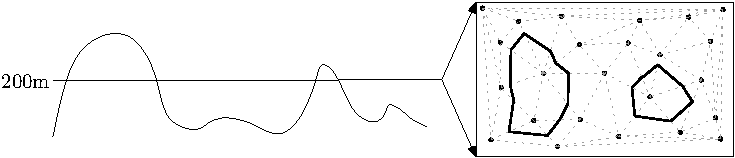
\includegraphics[width=0.95\textwidth]{figs/isoline}
  \caption{Cross-section of a terrain (left), and the 200m isoline extracted from a TIN (right).} 
\labfig{fig:isoline}
\end{figure}
the idea is to compute the intersection between the level value (\eg\ 200m) and the terrain, represented for instance with a TIN\@. 
Each triangle is scanned and segment lines are extracted to form an approximation of an isoline.


%%%
%
\section[TIN versus raster]{TIN versus raster for modelling terrains}

There is an ongoing debate about whether TINs or rasters are the better data model to model terrains.
Practitioners and scientists are probably split 50/50 on the issue.

A data model will be judged more \emph{efficient} than another if it represents a surface more accurately within the same amount of storage space, measured in bytes.
This of course depends on the data structure used to store that data model.

It should be said that both TIN and raster have advantages and disadvantages (as we will see during this course), and in practice one should choose the most appropriate model for the task at hand.
This means converting between the two data models when it is necessary (topic of \refchap{chap:conversion}).


%%%
%
\section{Notes and comments}

\citet{Kumler94} carried out a 4-year comparison between TINs and rasters.
He states that the common belief that a TIN is more space-efficient than raster is handicapped by the fact that a TIN must have \emph{at least} 3 times less points to be of equal space.
His conclusions are also that rasters can estimate elevation more accurately than comparably-sized TINs.
However, he still finishes with by stating: ``Yeah, well\ldots\ TINs still \emph{look} better.'' 

\citet{Fisher97} discusses the disadvantages of rasters, in a GIS and remote sensing context.

\citet{Frank92,Goodchild92a} discuss at lenght the issue of data model, data structure and representation of reality. 

\citet{Tse04} coined the term `2.75D GIS' and show an example of a where a triangulation is used to represent the surface of the Earth, with holes (for tunnels), cliffs and caves. 
The same idea is also referred to as a `2.8D GIS' by \citet{Groger05}.

While more an academic exercise then something used in practice, multi-resolution triangulation have been described and used for some application by \citet{DeFloriani02}.

\citet{Akima78} shows the advantages of using higher-order functions in each region of a TIN, to construct a $C^1$ or $C^2$ field. 

\citet{Dakowicz03} demonstrate that using simple rules (nearest-neighbour for instance) yields fields that are not realistic and have bad slope, which is in practice problematic for several applications.
Obtaining good slope from contour lines is possible, but is in practice a complex process.
% In other words, if elevation is the attribute modelled, the slope of the terrain will be `good', which is important for several applications, for example flood modelling.


%%%
%
\section{Exercises}

\begin{enumerate}
  \item Explain in our own words why a point cloud (\eg\ collected with airborne lidar) is not considered a complete representation of a terrain.
  \item What is a bivariate function? 
  \item Assume you have 2.75D terrain of an area. Is it possible to extract the isolines from it? What properties will these have? Will they intersect?
\end{enumerate}

%!TEX root = ../terrainbook.tex
% chktex-file 46


\setchapterpreamble[u]{\margintoc}

\graphicspath{{acquisition/}}


\chapter{Acquisition of elevation measurements}%
\label{chap:acquisition}

The very first step in the process of terrain modelling is the acquisition of elevation measurements. 
Nowadays, these measurements are usually collected in large quantities using some form of remote sensing, \ie\ sensors that measure---in our case---the distance to the Earth's surface from an airborne or even a spaceborne platform. 
In raw form, elevation measurements are typically stored as a point cloud, \ie\ a collection of georeferenced 3D points with each point representing one elevation measurement on the Earth's surface.

There are a number of remote sensing techniques that are used to measure elevation on Earth or other planets. 
Typically, these techniques measure
\begin{enumerate}
	\item the distance to the target surface; 
	\item their own position and orientation with respect to some global reference system. 
\end{enumerate}
By combining these, we can compute the 3D coordinates of the measured location on the target surface. 

In this chapter we will focus primarily on lidar, the most common acquisition technique for large scale terrain models with centimetre level accuracy. 
But we also give an overview of other acquisition techniques, for example photogrammetry, InSAR, and sonar. 
And to conclude we will look at typical artefacts that you might encounter while working with elevation data. 
This is because, as with any kind of real-world measurements, there are various uncertainties and restrictions in the acquisition process that lead to distortions---the \emph{artefacts}---in the acquired data. These artefacts need to be taken into account when further processing and using the elevation data. 
%This often makes further processing of the data more difficult, because these artefacts often violate assumption that are made in the DTM algorithms used to further process and analyse the point cloud, leading to erroneous results. 
% It is important that you are aware of these artefacts while working with elevation data, because only then you will be able to make the right modelling decisions. 
%Section~\ref{sec:artefacts} gives an overview of common problems in elevation data.

\section{Principles of lidar}%
\label{sec:lidar-principles}\index{lidar}

A lidar system\sidenote{While `lidar' is often treated as the acronym of \textbf{li}ght \textbf{d}etection \textbf{a}nd \textbf{r}anging, it actually originated as a portmanteau of `light' and `radar'. (from \href{https://en.wikipedia.org/wiki/Lidar\#History\_and\_etymology}{Wikipedia})} measures the distance to a target by illuminating it with pulsed laser light and measuring the reflected or \emph{backscattered}\sidenote{Backscattering is the natural phenomenon of  the reflection of (electromagnetic) waves or signals back to the direction they came from.} signal with a sensor (see Figure~\ref{fig:acqLidar}). 
\begin{marginfigure}
	\centering
	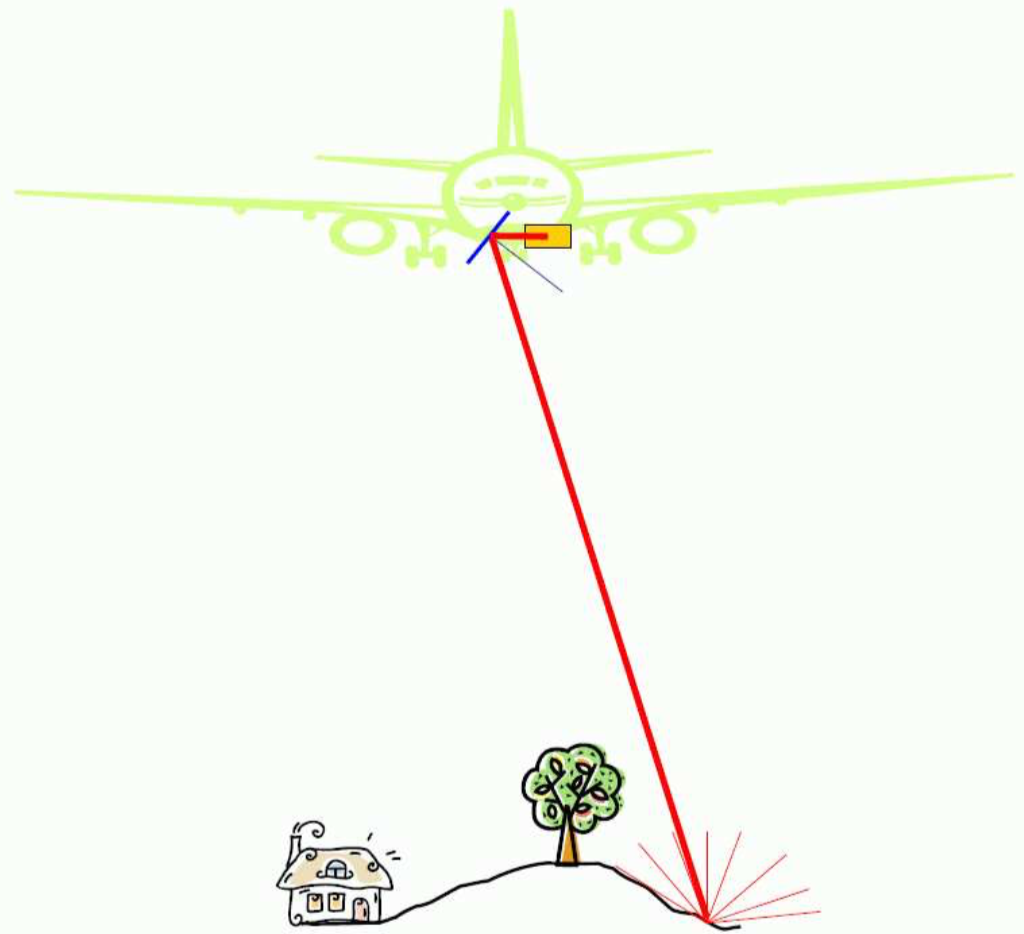
\includegraphics[width=\textwidth]{figs/lidar.png}
	\caption{Lidar range measurement}%
	\label{fig:acqLidar}
\end{marginfigure}
By measuring the time-of-flight, \ie\ the difference in time between emitting a pulse and detecting its return or \emph{echo}, the distance to the target that reflected the pulse can be found using a simple formula. To be exact, the time-of-flight $T$ is equal to
\begin{equation}
	\label{eq:tof}
	T= 2 \frac{R}{c}
\end{equation}
where $c$ is the speed of  light (approximately 300,000 km/s), and $R$ is the distance or \emph{range} between the lidar scanner and the target object that reflects the laser pulse. Therefore the range $R$ can be found from the measured time-of-flight $T$ using
\begin{equation*}
	R = \frac{1}{2} Tc.
\end{equation*}
A typical lidar systems performs hundreds of thousands of such range measurements per second. 

Lidar scanners exist in various forms. 
They can be mounted on a static tripod (terrestrial lidar) for detailed local scans, or on a moving platform such as a car (mobile lidar) or an aircraft (airborne lidar) for rapid scanning of larger areas. Nowadays, also hand-held lidar systems exist, and even some of the latest smartphones  have a lidar sensor. 
Furthermore, lidar can also be used from a satellite in space\sidenote{NASA has used space lidar \href{https://en.wikipedia.org/wiki/ICESat-2}{on Earth}, \href{https://lola.gsfc.nasa.gov}{on the Moon}, and \href{https://en.wikipedia.org/wiki/Mars_Orbiter_Laser_Altimeter}{on Mars}.}. 

However, in the remainder of this text we will focus on airborne lidar.


%%%
%
\subsection{Georeferencing the range measurements}

\begin{figure}
	\centering
	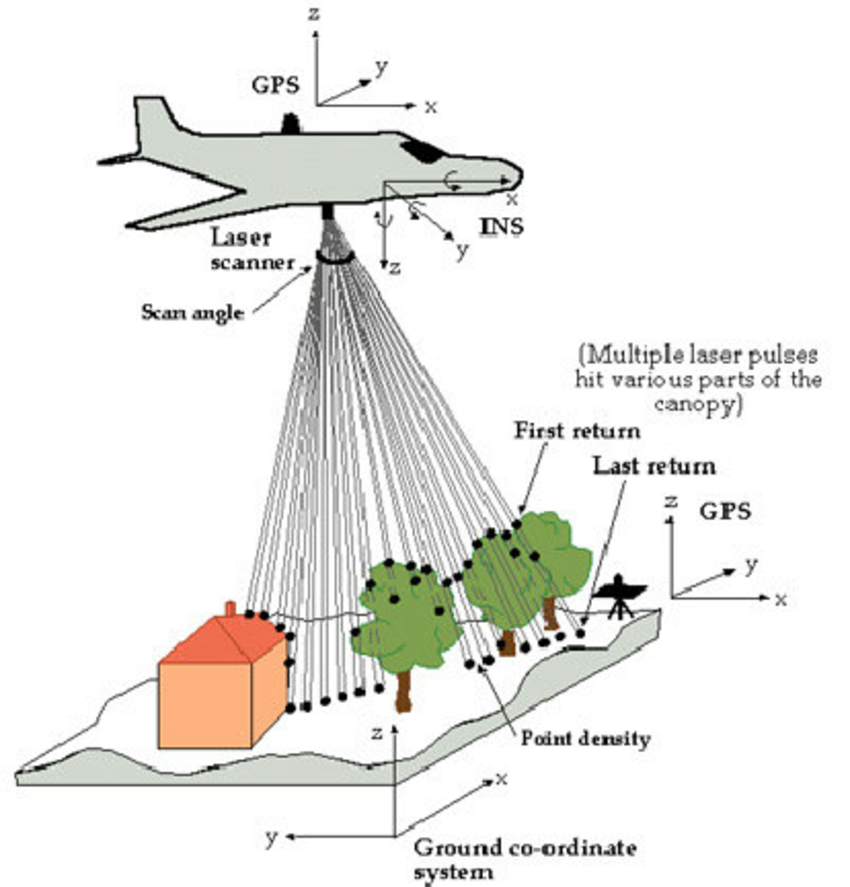
\includegraphics[width=0.7\textwidth]{figs/lidar-gnss-imu.png}
	\caption{An airborne lidar system. Figure from \citet{Dowman04}.}%
\label{fig:airborne-lidar}
\end{figure}
Apart from the  laser scanner itself, a lidar  system uses a GPS receiver and an inertial navigation system (INS), see Figure~\ref{fig:airborne-lidar}. 
\marginnote{inertial navigation system (INS)}\index{inertial navigation system (INS)}
These devices, which respectively provide the global position and orientation of the laser scanner, are needed for georeferencing, \ie\ to convert the range measurements of the laser scanner to 3D point measurements in a global coordinate system such as WGS84. 

To  obtain an accurate global position, \emph{differential GPS} (DGPS) is employed. 
\marginnote{differential GPS}\index{differential GPS}
DGPS is a technique to enhance the accuracy of GPS  by using GPS stations on the ground (one is visible in Figure~\ref{fig:airborne-lidar}). 
These DGPS stations have a known position and they broadcast the difference between that  known position and the position at the station as indicated by GPS\@. 
This difference is essentially a correction for errors in the GPS signal. The aircraft receives these differences from nearby DGPS stations and uses them to correct the GPS position of the aircraft. Using DGPS the accuracy of the GPS position on the aircraft can be improved from around 15 meters to several centimetres.

To obtain the accurate orientation of the laser scanner, the INS of the aircraft is used. 
The INS accurately measures the orientation, \ie\ the yaw, pitch  and roll angles of the aircraft, by means of an inertial measurement unit (IMU)\sidenote{\url{https://en.wikipedia.org/wiki/Inertial_measurement_unit}}. 
\marginnote{inertial measurement unit (IMU)}\index{inertial measurement unit (IMU)}
Only when we accurately know the orientation of the laser scanner, can we know the direction (in a global coordinate system) in which a laser pulse is emitted from the aircraft.

By combining the global position and the global orientation of the laser scanner with the range measurement from the laser scanner, the georeferenced 3D position of  the point  on the target object that reflected the lase pulse can be computed.


%%%
\subsection{Echo detection}

A lidar system performs ranging measurements using the time-of-flight principle that allows us to compute range from a time measurement using the known speed of light in the air. 
The time measurement starts when the laser pulse is emitted and is completed when a backscattered echo of that signal is detected. 
In practice one emitted pulse can even lead to multiple echoes  in the case when an object reflects part of the laser pulse, but also allows part of the pulse to continue past the object. 
Notice that lidar pulses are typically emitted in a slightly divergent manner. As a result the footprint of the pules at ground level is several centimetres in diameter, which increases the likelihood of multiple echoes.

\begin{figure}
	\centering
	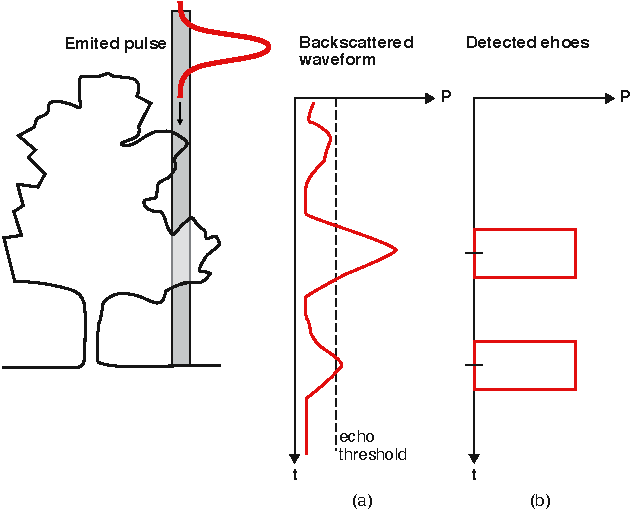
\includegraphics[width=0.8\textwidth]{figs/lidar-multipulse.pdf}
	\caption{The emitted laser pulse, \textbf{(a)} the returned signal, and \textbf{(b)} the recorded echoes. Figure adapted from \citet{Bailly12}.}%
\label{fig:lidar-multipulse}
\end{figure}
Figure~\ref{fig:lidar-multipulse} illustrates what the backscattered signal looks like when it hits a target object in the shape of a tree. 
A tree is particularly interesting because it often causes multiple echoes (one or more on its branches and one on the ground below).  The lidar sensor observes a waveform that represents the received signal power ($P$) as a function of time ($t$). 
With the direct detection lidar systems that we focus on in this book, the echoes are derived from the backscattered waveform by using a thresholding technique. This essentially means that an echo is recorded whenever the power of the waveform exceeds a fixed threshold (see Figure~\ref{fig:lidar-multipulse}b). 

An echo can  also  be referred to as a \emph{return}. 
\marginnote{return}\index{return}
For each return the return count is recorded, \eg\ the first return is the first echo received from an emitted laser pules and the last return is the last received echo (see Figure~\ref{fig:lidar-multipulse}). The return count can in some cases be used to determine if an echo was reflected on vegetation or ground (ground should then be the last return).


%%%
\subsection{Anatomy of a lidar system}%
\label{lidar:anatomy}


A lidar system consists of an optical and an electronic part. 
As shown in Figure~\ref{fig:lidar-components}, each part consists of several components.
\begin{figure}
	\centering
	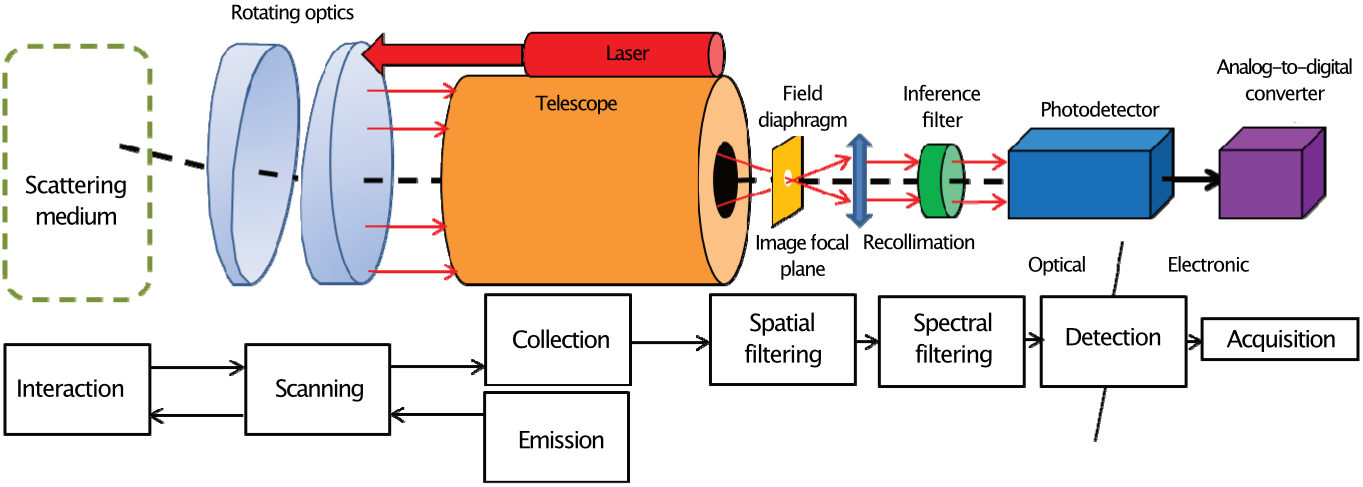
\includegraphics[width=\textwidth]{figs/lidar-components.png}
	\caption{Conventional architecture of a direct detection lidar system. Figure from \citet{Chazette16}.}%
\label{fig:lidar-components}
\end{figure}

In the optical part, a pulse of a particular wavelength (typically near-infrared) is generated by the laser source for each lidar measurement. 
It then passes through a set of  optics (lenses and mirrors) so that it leaves the scanner in an appropriate direction. 
After the pulse interacts with the scattering medium, it is reflected back into the scanning optics which then directs the signal into a telescope. 
The telescope converges the signal through a field diaphragm (essentially a tiny hole around the point of convergence). 
The field diaphragm blocks stray light rays (\eg\ sunlight reflected into the optics from any angle) from proceeding in the optical pipeline. 
Next, the light signal is recollimated so that it again consists only of parallel light rays. 
The final step of the optical part is the inference filter which blocks all wavelengths except for the wavelength of the laser source. 
This is again needed to block stray light rays from distorting the measurement.

The electronic part consists of a photodetector, which first transforms the light signal into an electrical current, which is then converted to a digital signal using the analogue-to-digital converter. 
Once the digital signal is available, further electronics can be used to interpret and record the signal.


%%%
\subsection{Laser wavelength}

Choosing the optimal laser wavelength is a compromise of several different factors. 
One needs to consider atmospheric scattering, 
\marginnote{atmospheric scattering}\index{atmospheric scattering}
\ie\ how much of the signal is lost simply by travelling through the atmosphere, and the absorption capacity of vegetation, \ie\ how much of  the signal is lost because it is absorbed by vegetation. In addition, there is the stray signal due to direct and scattered contributions of sunlight. While it is possible to filter such stray signals in the lidar system to some degree, it remains wise to choose a wavelength that is only minimally affected by it. Finally there are regulations that limit the laser radiance values permissible to the eye. This means that the power of emitted signal needs to be carefully controlled, and/or a wavelength must be chosen that  is not absorbed by the eye so much.

As a result, most lidar systems use a wavelength in the near-infrared spectrum, usually between 600 and 1000 nm. A notable exception is made for bathymetric purposes, in which case a green (532 nm) laser is used because that has a greater penetration ability in water.

\subsection{Scanning patterns}
In order to improve the capacity to quickly scan large areas, a number of rotating optical elements are typically present in a lidar system. Using these optical elements, \ie\  mirrors or prisms, the emitted laser pulse is guided in a cross-track direction (\ie\ perpendicular to the along-track direction in which  the aircraft moves, see Figure~\ref{fig:acqLidar}),  thereby greatly increasing the scanned ground area  per travelled meter of the aircraft.
Figure~\ref{fig:lidar-patterns} depicts a number of possible configurations of rotating optics and shows the resulting scanning patterns. It is clear that density of points on the ground is affected by the scanning pattern. The top example for example, yields much higher densities on edges of the scanned area. In practice more uniform patterns, such  as the bottom two examples are often preferred.

\begin{figure}
	\centering
	\includegraphics[width=0.7\textwidth]{figs/lidar-patterns.pdf}
	\caption{Different configurations of rotating mirrors and the associated scanning patterns from a moving platform. Arrows indicate the direction of the emitted laser signal. Figure from \citet{Chazette16}.}%
\label{fig:lidar-patterns}
\end{figure}



\begin{kaobox-toread}[frametitle=\faExternalLink\ To read or to watch]
	This YouTube video explains the principles of an aerial LiDAR system:
	\\
	\url{https://youtu.be/EYbhNSUnIdU}
\end{kaobox-toread}


% TODO : put a side-by-side with vegetation and without lidar to show DTM and DSM


\section{Other acquisition techniques}%
\label{sec:acquisistion-techniques}

Apart from lidar there are also other sensor techniques that can be used to acquire elevation data. Some of these are  active sensors just like lidar (a signal is generated and emitted from the sensor), whereas others are passive (using the sun as light source). And like lidar, these sensors themselves only do range measurements, and need additional hardware such as a GPS receiver and an IMU to georeference the measurements. What follows is a brief description of the three other important acquisition techniques used in practice. 

% FIXME image with flight parameters and strips

\subsection{Photogrammetry}%
\label{sec:photogrammetry}\index{photogrammetry}
\begin{marginfigure}
	\centering
	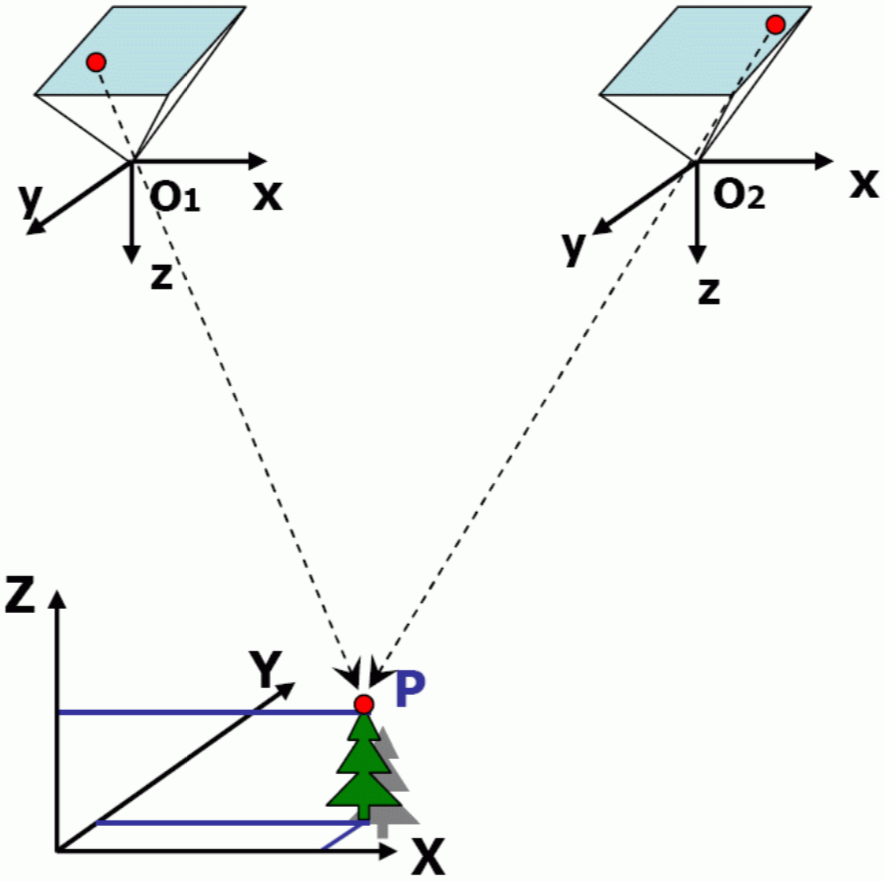
\includegraphics[width=\textwidth]{figs/photogrammetry.png}
	\caption{Photogrammetry}%
	\label{fig:acqPhoto}
\end{marginfigure}
Photogrammetry allows us to measure the distance from overlapping photographs taken from different positions. 
If a ground point, called a \emph{feature}, is identifiable in two or more images, its 3D coordinates can be computed in two steps. 
First, a viewing ray for that feature must be reconstructed for each image. 
A viewing ray can be defined as the line from the feature, passing through the projective centre of the camera, to the corresponding pixel in the image sensor (see Figure~\ref{fig:acqPhoto}). 
Second, considering that we know the orientation and position of the camera, the distance to the feature (and its coordinates) can be computed by calculating the spatial intersection of several viewing rays.

% interior orientation (camera parameters such as focal length) and the exterior orientation (camera position and orientation)

The number of 3D point measurements resulting from photogrammetry thus depends on the number of features that are visible in multiple images, \ie\ the so-called matches.
With \emph{dense image matching} 
\marginnote{dense image matching}\index{dense image matching}
it is attempted to find a match for every pixel in an image. 
If the ground sampling distance, \ie\ the pixel size on ground level, is small (around \SI{5}{\cm} for state-of-the-art systems), point densities of hundreds of points per square meter can be achieved, which is much higher than the typical lidar point cloud (typically up to dozens of points per square meter). 

In photogrammetry we distinguish between \emph{nadir} images, 
\marginnote{nadir images}\index{nadir images}
that are taken in a direction straight down from the camera, and \emph{oblique}
\marginnote{oblique images}\index{oblique images}
images that are taken at an angle with respect to the nadir direction.
Vertical features such as building façades are only visible on oblique images.
Therefore, oblique images are needed if one wants to see building façades in a dense image matching point cloud.

Because photography is used, photogrammetry gives us also the colour of the target surface, in addition to the elevation.
This could be considered an advantage over lidar which captures several attributes for each point (\eg\ the intensity of measured laser pulse and the exact GPS time of measurement), but colour is not among them.

Both airborne and spaceborne photogrammetry are possible.

%%%
\subsection{InSAR}%
\label{sec:insar}%
\index{InSar}

Interferometric synthetic aperture radar (InSAR) is a radar-based technique that is used from space in the context of terrain generation. 
It is quite different from airborne lidar or photo\-gramme\-try-based acquisition because of the extremely high altitude of the satellite carrying the sensor. 
Signals have to travel very long distances through several layers of unpredictable atmospheric conditions. 
As a result the speed of the radar signal is not known and the time-of-flight principle can not be used to get detailed measurements. 
However, by using a comprehensive chain of processing operations based on the measured phase shifts and the combination of multiple InSAR images, accurate elevation can still be measured. 
With InSAR it is possible to cover very large regions in a short amount of time, \eg\ the global SRTM\sidenote{\url{https://en.wikipedia.org/wiki/Shuttle_Radar_Topography_Mission}} dataset was generated with InSAR\@. 
Compared to dense image matching and lidar, InSAR-derived DTMs usually have a much lower resolution, \eg\ SRTM has a pixel size of 30 meters.

%%
\begin{kaobox-toread}[frametitle=\faExternalLink\ To read or to watch]
	\href{https://en.wikipedia.org/wiki/Interferometric_synthetic-aperture_radar}{Wikipedia page about \emph{Interferometric synthetic-aperture radar}}.
\end{kaobox-toread}


%%%
\subsection{Echo sounding}%
\label{sec:mbes}
Echo sounding is a form of sonar that can be used for bathymetry, \ie\ mapping underwater terrains from a boat. 
Similar to lidar, it uses the time-of-flight principle to compute distance, but sound is used instead of light. 

Single-beam and multi-beam echo sounders exist. Multi-beam systems are capable of receiving many narrow sound beams from one emitted pulse. As a result it measures the target surface much more accurately. 
For bathymetry usually a multi-beam echo sounder is used.

Chapter~\ref{chap:bathymetry} describes techniques to process bathymetric datasets and create terrain of the seabed.

%%
\begin{kaobox-toread}[frametitle=\faExternalLink\ To read or to watch]
  The principles of echo sounding.
  \\
  \url{https://en.wikipedia.org/wiki/Echo_sounding}
\end{kaobox-toread}




\section{Artefacts}%
\label{sec:artefacts}

In the acquisition process, there are many aspects---both under our control and not under our control--- that affect the quality and usability of the resulting elevation data for a given application. 
Some examples are
\begin{itemize}
	\item the choice of the sensor technique, 
	\item the sensor specifications, \eg\ the resolution and focal length of a camera, or the scanning speed, the width of the swath, and scanning pattern of a lidar system,
	\item the flight parameters, \eg\ the flying altitude and the distance and overlap between adjacent flights,
	\item atmospheric conditions, 
	\item the physical properties of the target surface.
\end{itemize}

An artefact is any error in the perception or representation of information that is introduced by the involved equipment or techniques. 
Artefacts can result in areas without any measurements (\eg\ the \emph{no-data} values in a raster), or in so-called \emph{outliers}, \ie\ sample points with large errors in their coordinates. 
\marginnote{outliers}\index{outliers}

We distinguish three types of artefacts, 
\begin{enumerate}
	\item those that occur due to problems in the sensor, 
	\item those that occur due to the geometry and material properties of the target surface, 
	\item those that occur due to post-processing steps.
\end{enumerate}

% Active/passive sensors
% different platforms ground/airborne/space
% different physical principles
% pulse footprint, wavelength
% different sensor specs (resolution, speed) and operation specs (flight height etc)
% different cost, update cycles

\subsection{Sensor orientation}
The sensor position and orientation are continuously monitored during acquisition, \eg\  by means of GNSS and an IMU for airborne and seaborne systems, and used to determine the 3D coordinates of the measured points. 
Consequently, any errors in the position and orientation of the sensor platform affect the elevation measurements. 
For this reason adjacent flight strips (see Figure~\ref{fig:lidarStrips}) often need to be adjusted to match with each other using ground control points. 
\begin{figure}
	\centering
	\begin{subfigure}{0.4\linewidth}
		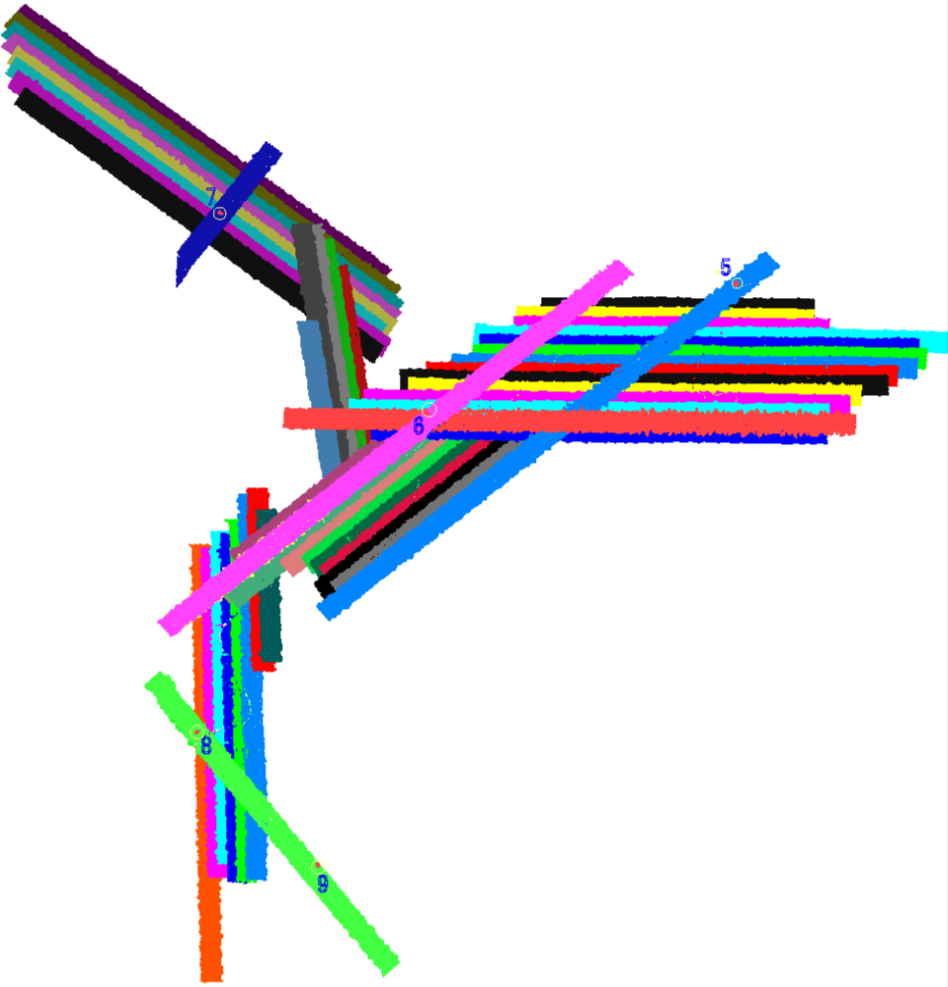
\includegraphics[width=\textwidth]{figs/lidar_strips.png}
		\subcaption{Plan view of the different strips of a lidar survey \citep{Kornus03}}\label{fig:lidarStrips}
	\end{subfigure}
	\quad
	\begin{subfigure}{0.4\linewidth}
		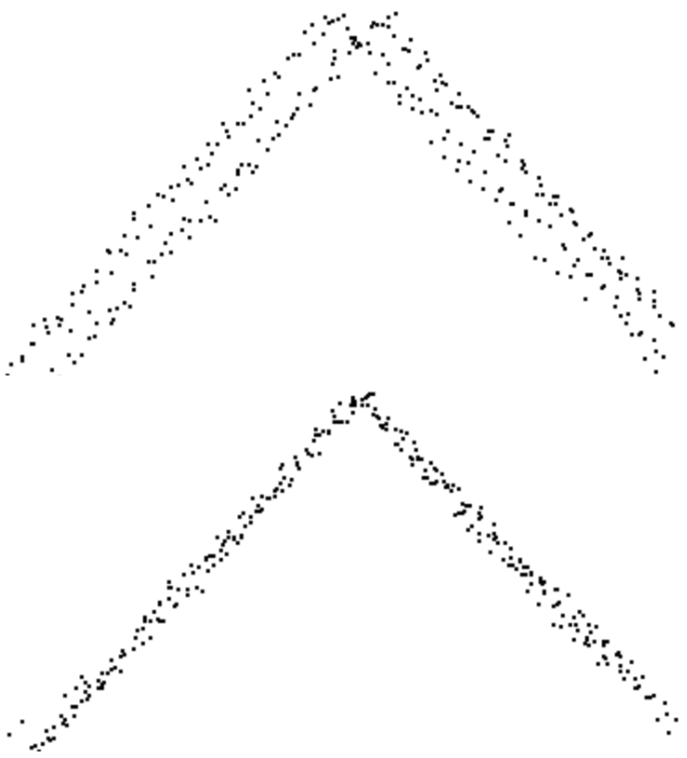
\includegraphics[width=\textwidth]{figs/strip_adjustment.png}
		\subcaption{Cross-section of gable roof before (top) and after (bottom) strip adjustment \citep{Vosselman02}}\label{fig:lidarGableRoof}
	\end{subfigure}
	\caption{Strip adjustment for lidar point clouds}%
\label{fig:lidarStripAdj}
\end{figure}
If the strip adjustments process fails or is omitted, a `ghosting' effect can occur as illustrated in Figure~\ref{fig:lidarGableRoof} (top). 
Photogrammetry knows a similar process called aerial triangulation, in which camera positions and orientation parameters (one set for each image) are adjusted to fit with each other. Errors in the aerial triangulation can lead to a noisy result for the dense matching as seen in Figure~\ref{fig:dim}.
\begin{figure*}
	\centering
	\begin{subfigure}{0.45\linewidth}
		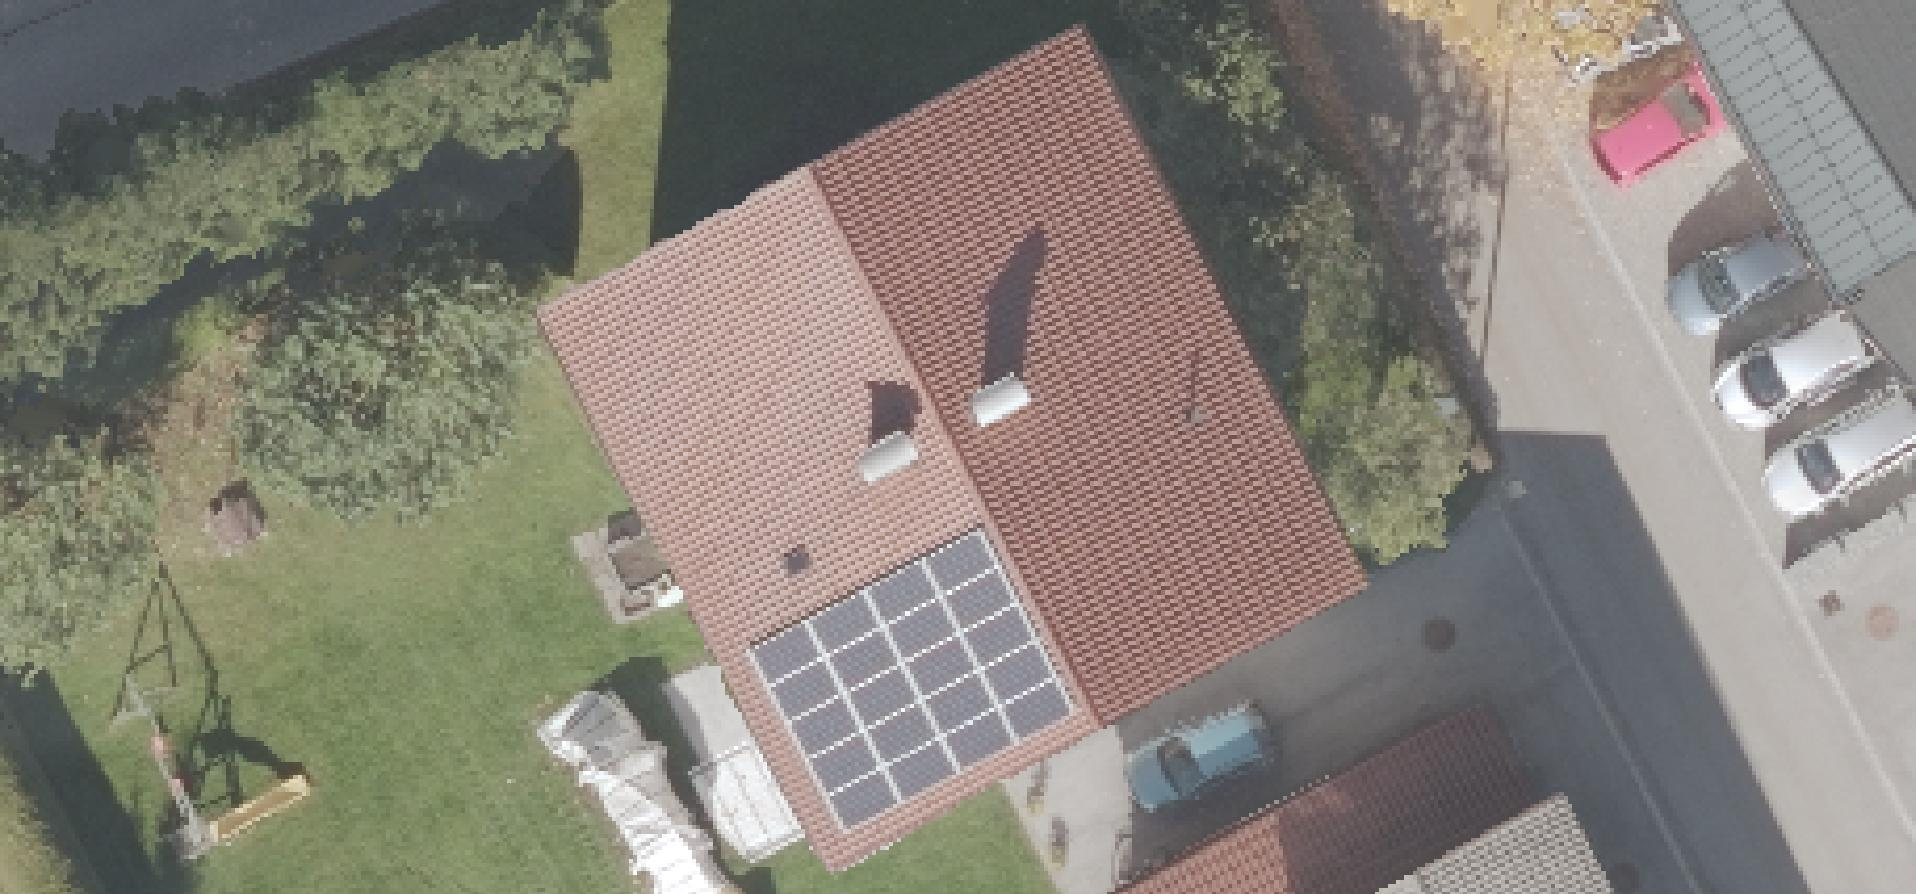
\includegraphics[width=\textwidth]{figs/Roof_OP_NA_10cm.jpg}
		\subcaption{Nadir image}\label{fig:dim:a}
	\end{subfigure}
	
	\begin{subfigure}{0.45\linewidth}
		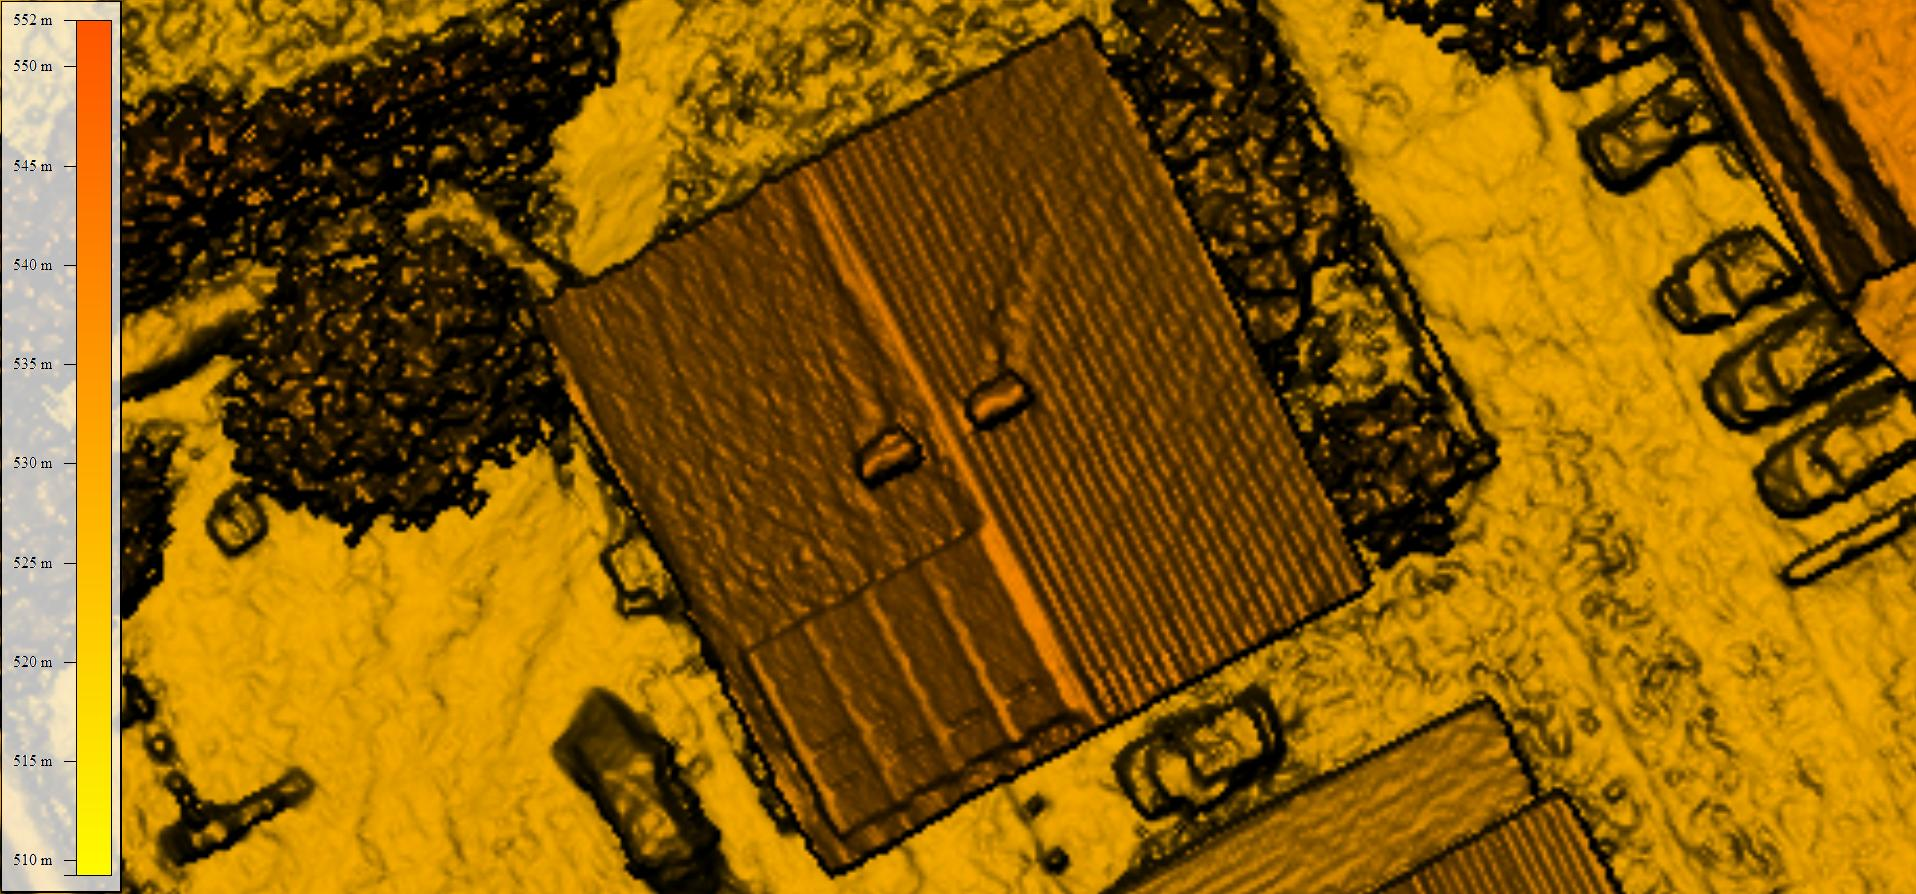
\includegraphics[width=\textwidth]{figs/Roof_DSM_NA_10cm.jpg}
		\subcaption{DSM with good aerial triangulation}\label{fig:dim:b}
	\end{subfigure}
	\quad
	\begin{subfigure}{0.45\linewidth}
		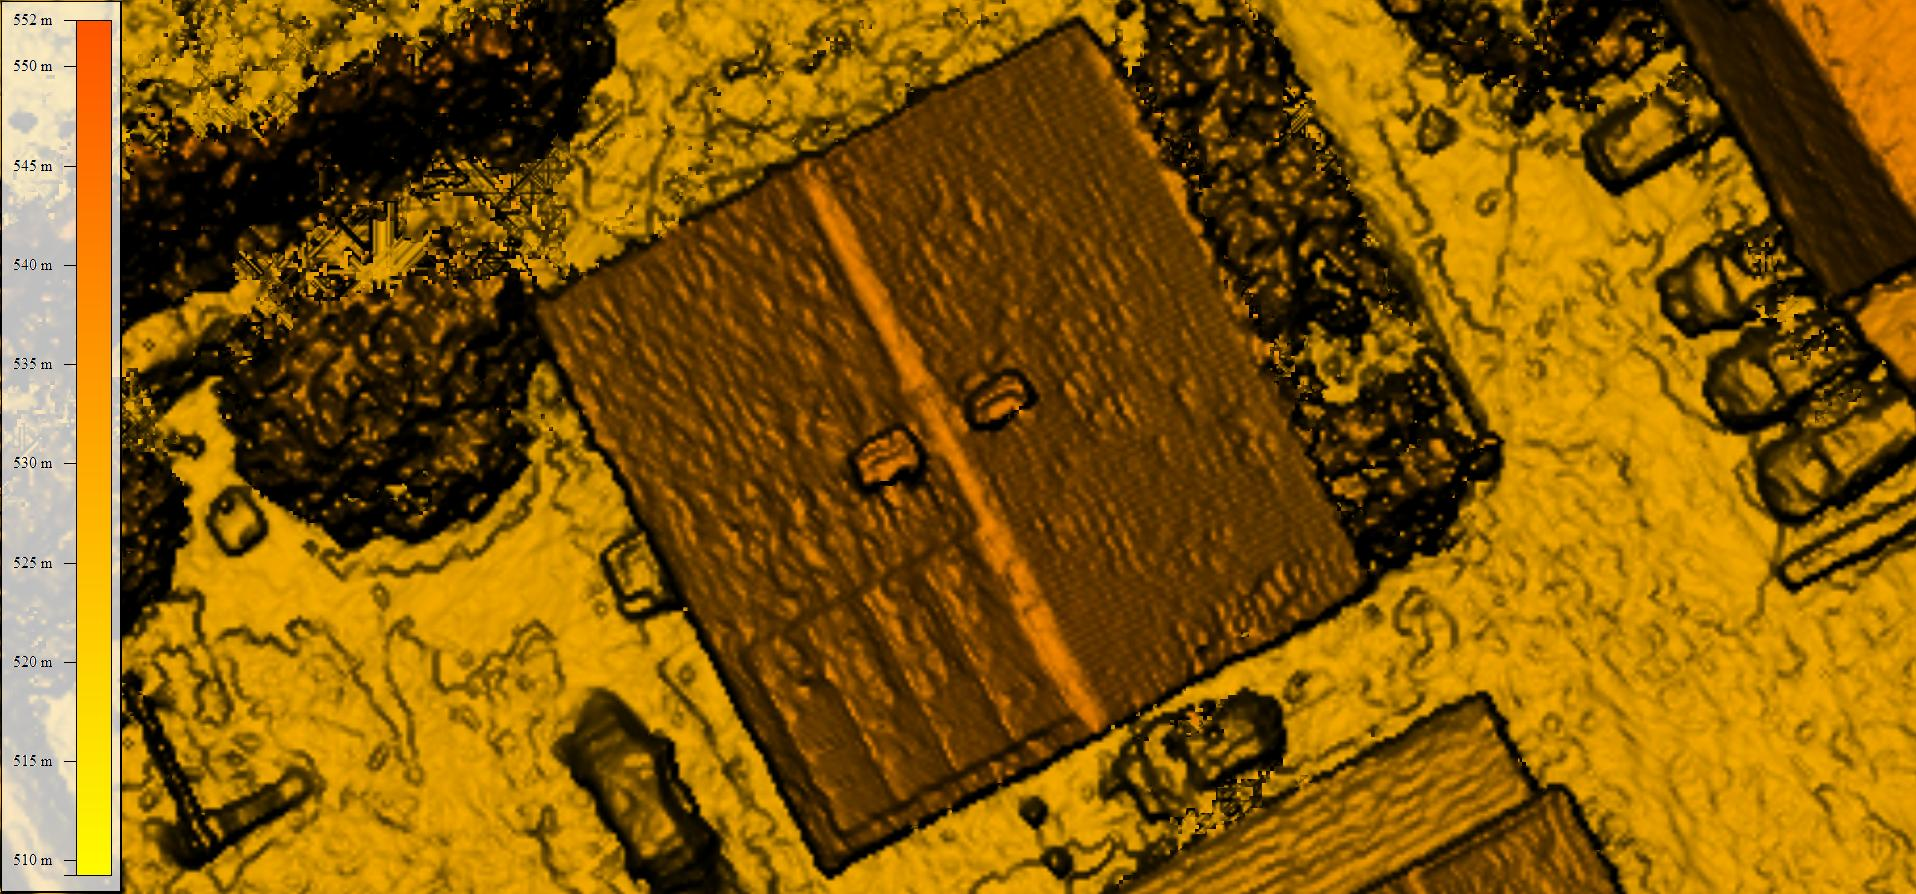
\includegraphics[width=\textwidth]{figs/Roof_DSM_NA+OBL_10cm.jpg}
		\subcaption{DSM with poor aerial triangulation}\label{fig:dim:c}
	\end{subfigure}
	\caption{Errors in aerial triangulation can lead to distortions in the DSM (derived from dense image matching). Images courtesy of Vermessung AVT.}%
\label{fig:dim}
\end{figure*}


\subsection{Target surface}
Many commonly occurring  artefacts  happen due to properties of the target surface. We distinguish three classes.

\subsubsection{Geometry} 
The shape of the target surfaces in relation to the sensor position has a great effect on 1) local point densities and 2) occlusion. As you can see from Figure~\ref{fig:lidarAcquisitionConditions:a},
\begin{marginfigure}
	\centering
	\includegraphics[width=\textwidth,page=2]{figs/lidarAcq.pdf}
	\caption{Point distribution and occlusion}%
	\label{fig:lidarAcquisitionConditions:a}
\end{marginfigure}
which illustrates this for lidar, surfaces that are closest to the scanner and orthogonal to the laser beams will yield the highest point densities (see the rooftop of the middle house). Very steep surfaces on the other hand, yield relatively low point densities (see the façades of the buildings). 

\emph{Occlusion} happens when a surface is not visible from the scanner position.% 
\index{occlusion}
As a result there will be gaps in the point coverage, also visible in Figure~\ref{fig:lidarAcquisitionConditions:a}. 
Notice how some steep surfaces and some of the adjacent ground are not registered at all by the scanner because it simply could not `see' these parts.

The severity of both effects mostly depends on the geometry of the target objects and flight parameters such as the flying altitude and the amount of overlap between flight strips.
However, regardless of what flight parameters are chosen for a survey both effects are almost always visible somewhere in the resulting dataset, see for example Figure~\ref{fig:pcd} for different lidar datasets for the same area.

% oblique vs nadir for occlusion
%Especially occlusion can be a problem for (2.5D) DTM generation because it causes no-data areas that may be problematic.

\begin{figure*}
	\centering
	\begin{subfigure}{0.45\linewidth}
		
\includegraphics[width=\textwidth]{figs/ahn1_d.png}
		\subcaption{AHN1 (1996--2003)}\label{fig:pcd:ahn1}
	\end{subfigure}
	\quad
	\begin{subfigure}{0.45\linewidth}
		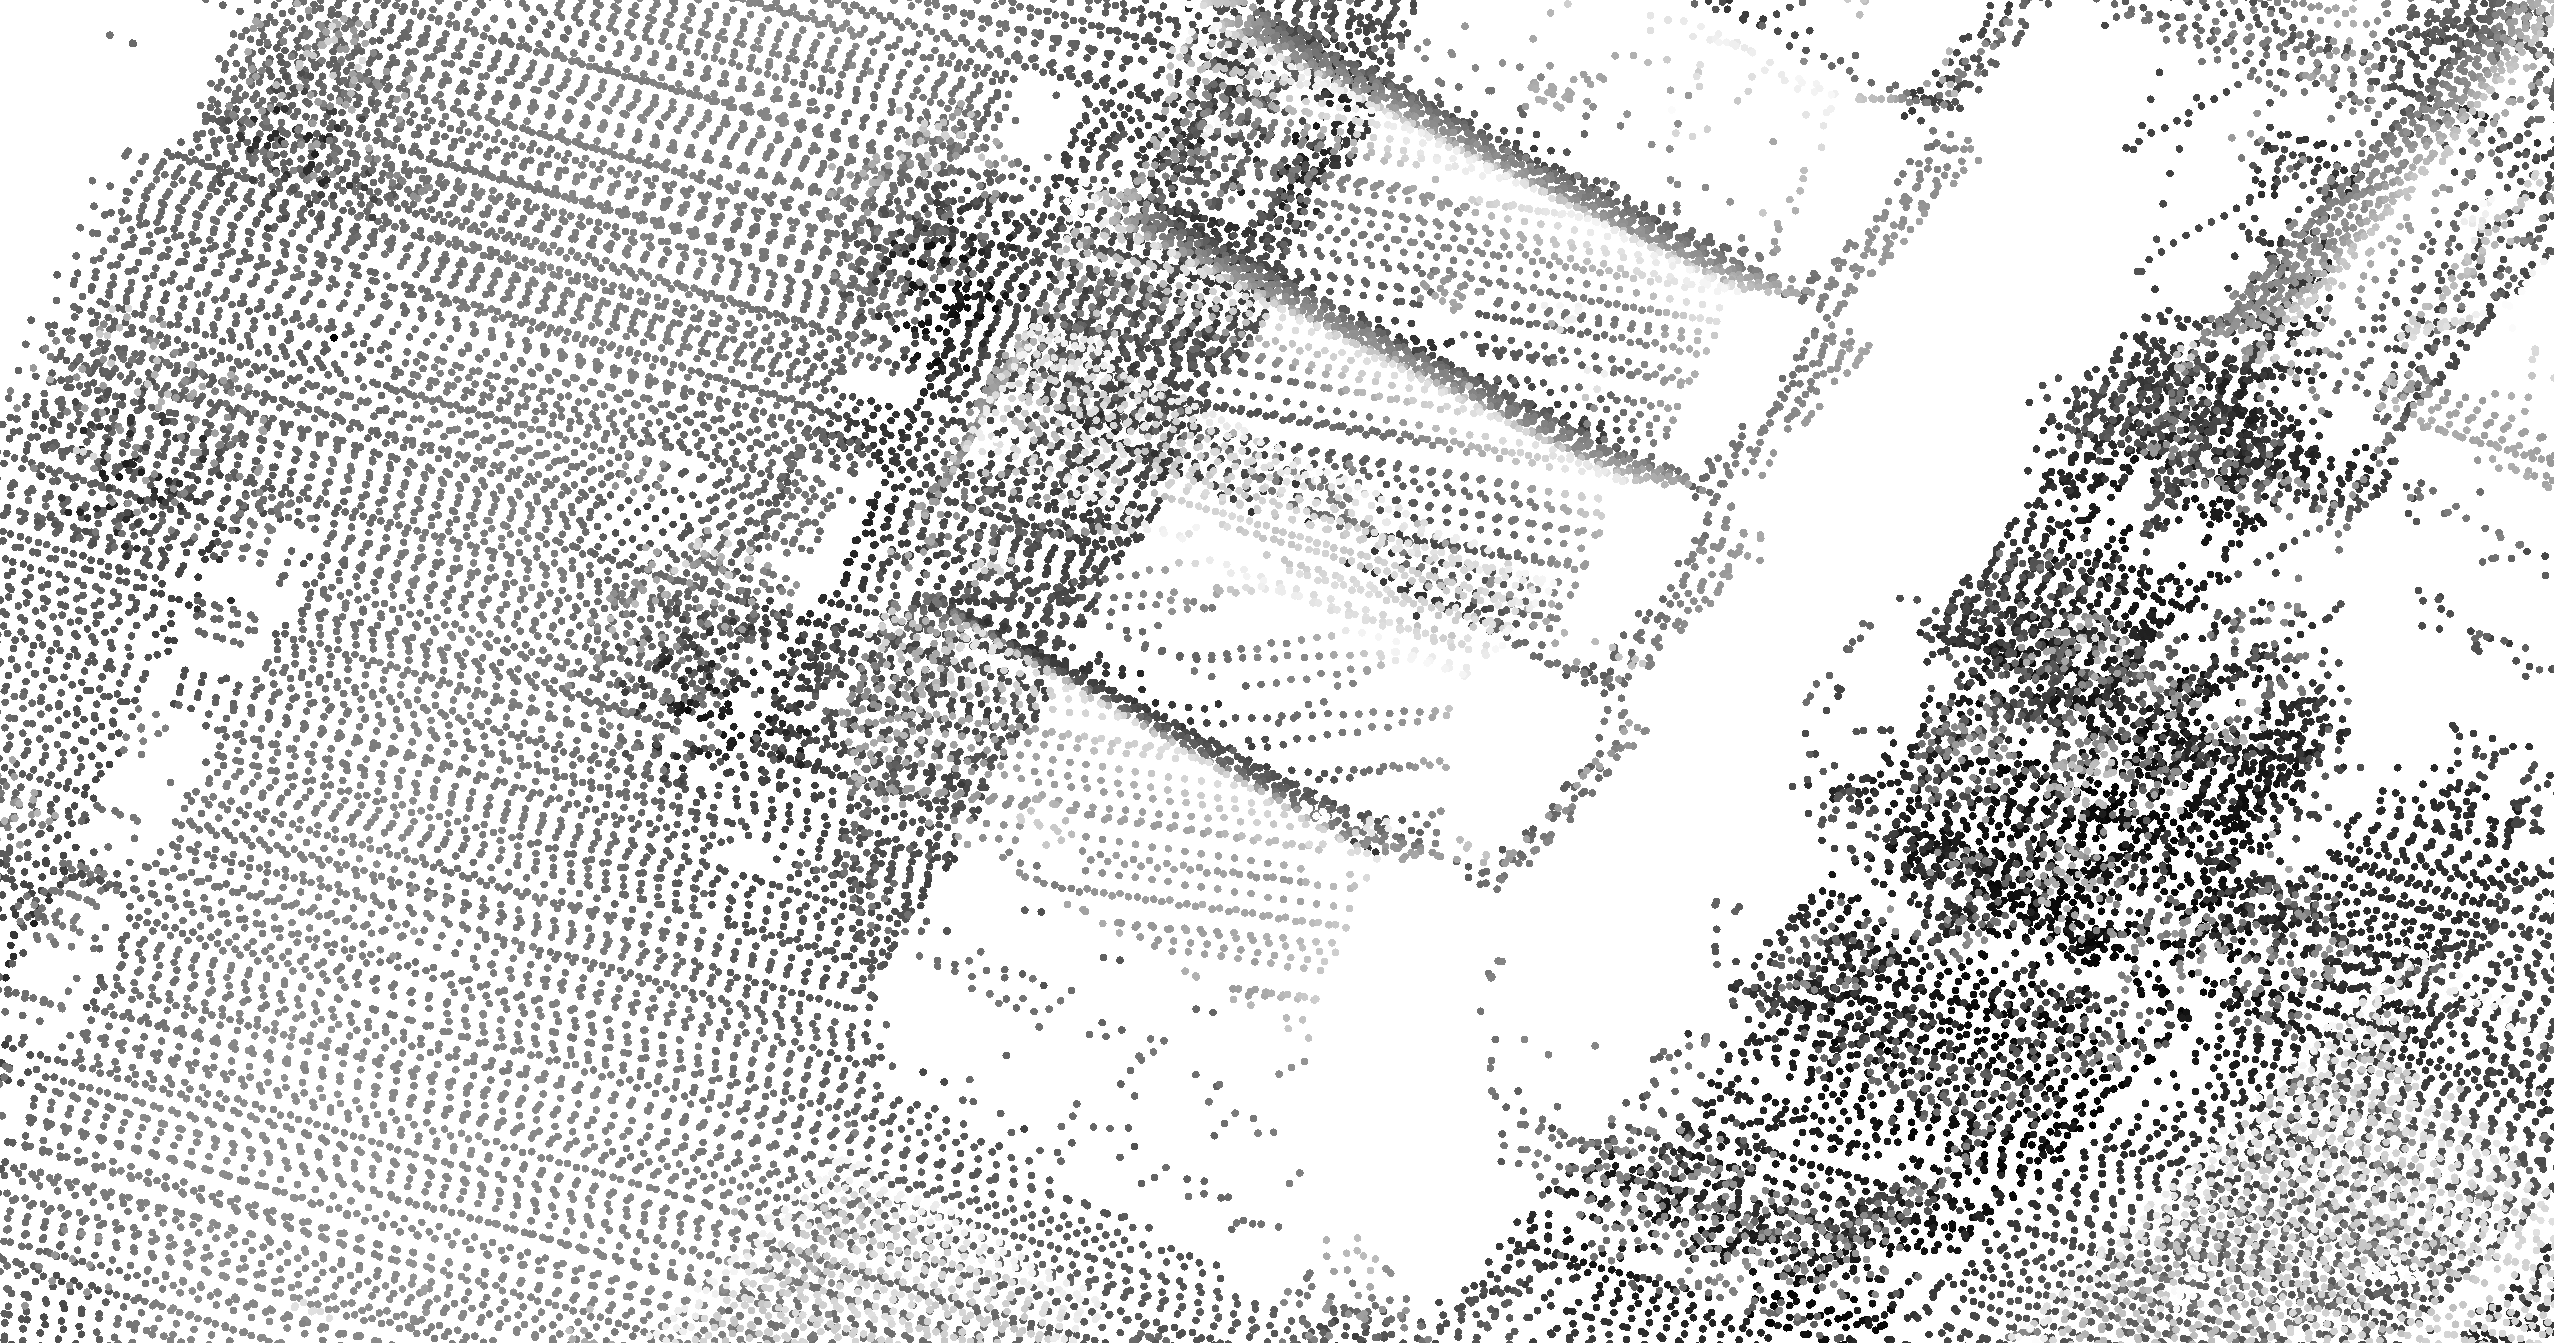
\includegraphics[width=\textwidth]{figs/ahn2_d.png}
		\subcaption{AHN2 (2008)}\label{fig:pcd:ahn2}
	\end{subfigure}
	
	\begin{subfigure}{0.45\linewidth}
		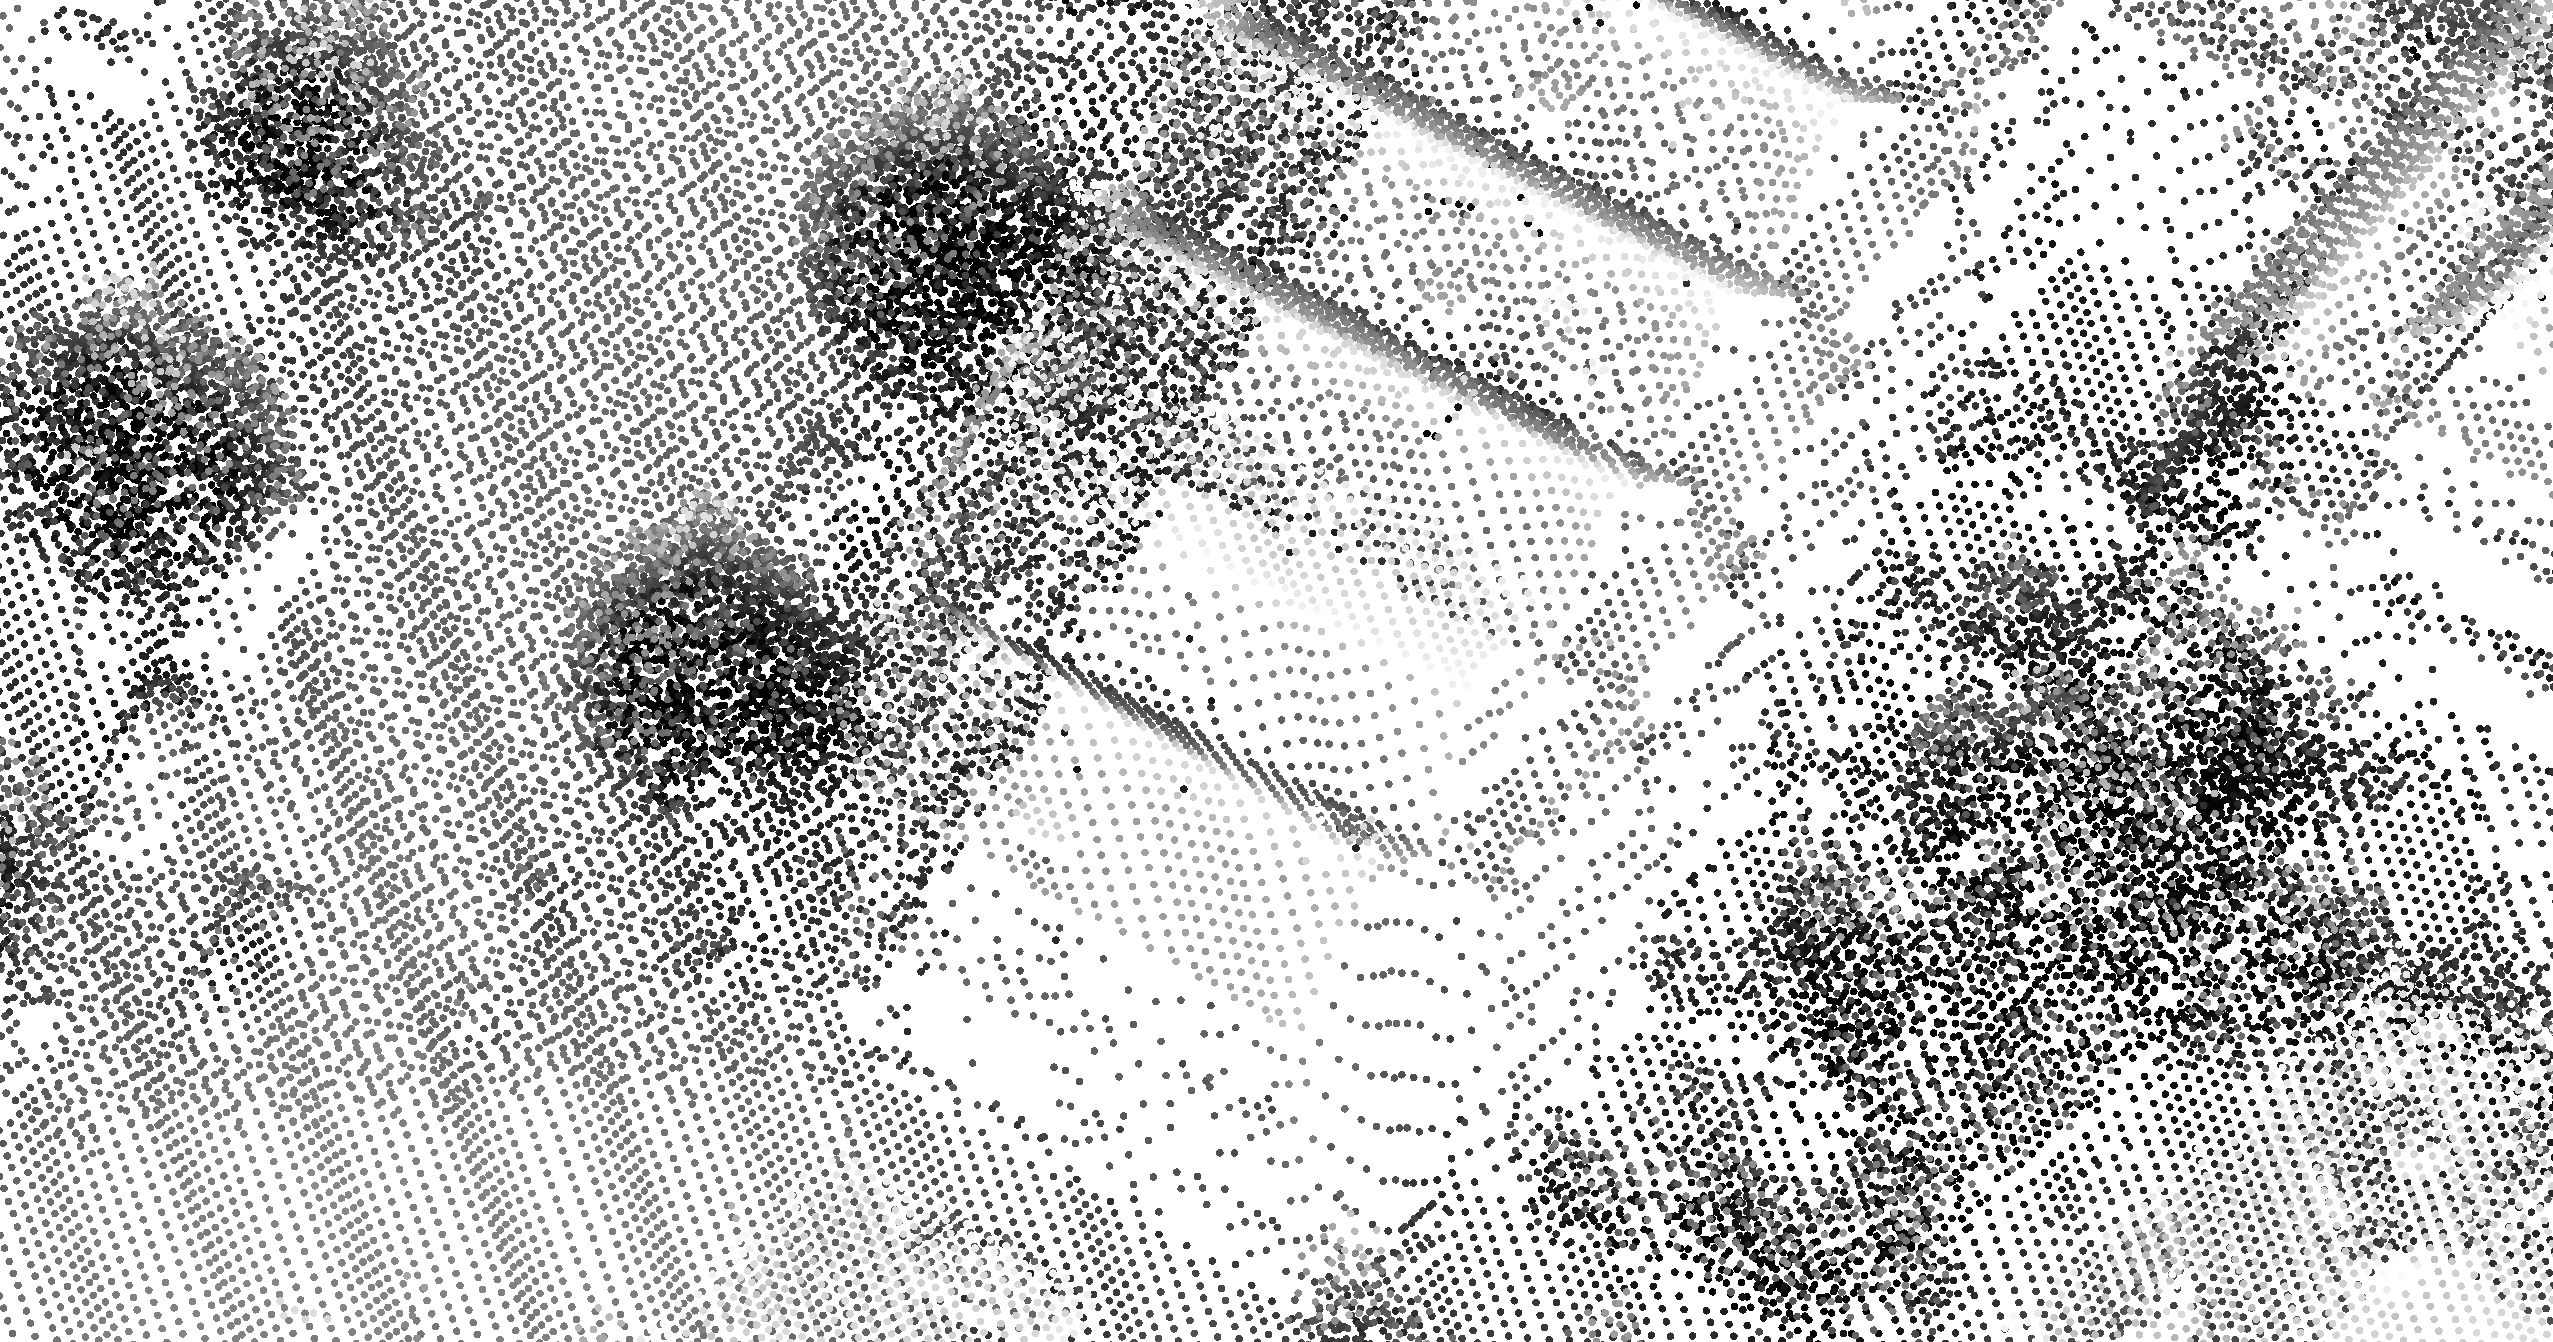
\includegraphics[width=\textwidth]{figs/ahn3_d.png}
		\subcaption{AHN3 (2014)}\label{fig:pcd:ahn3}
	\end{subfigure}
	\quad
	\begin{subfigure}{0.45\linewidth}
		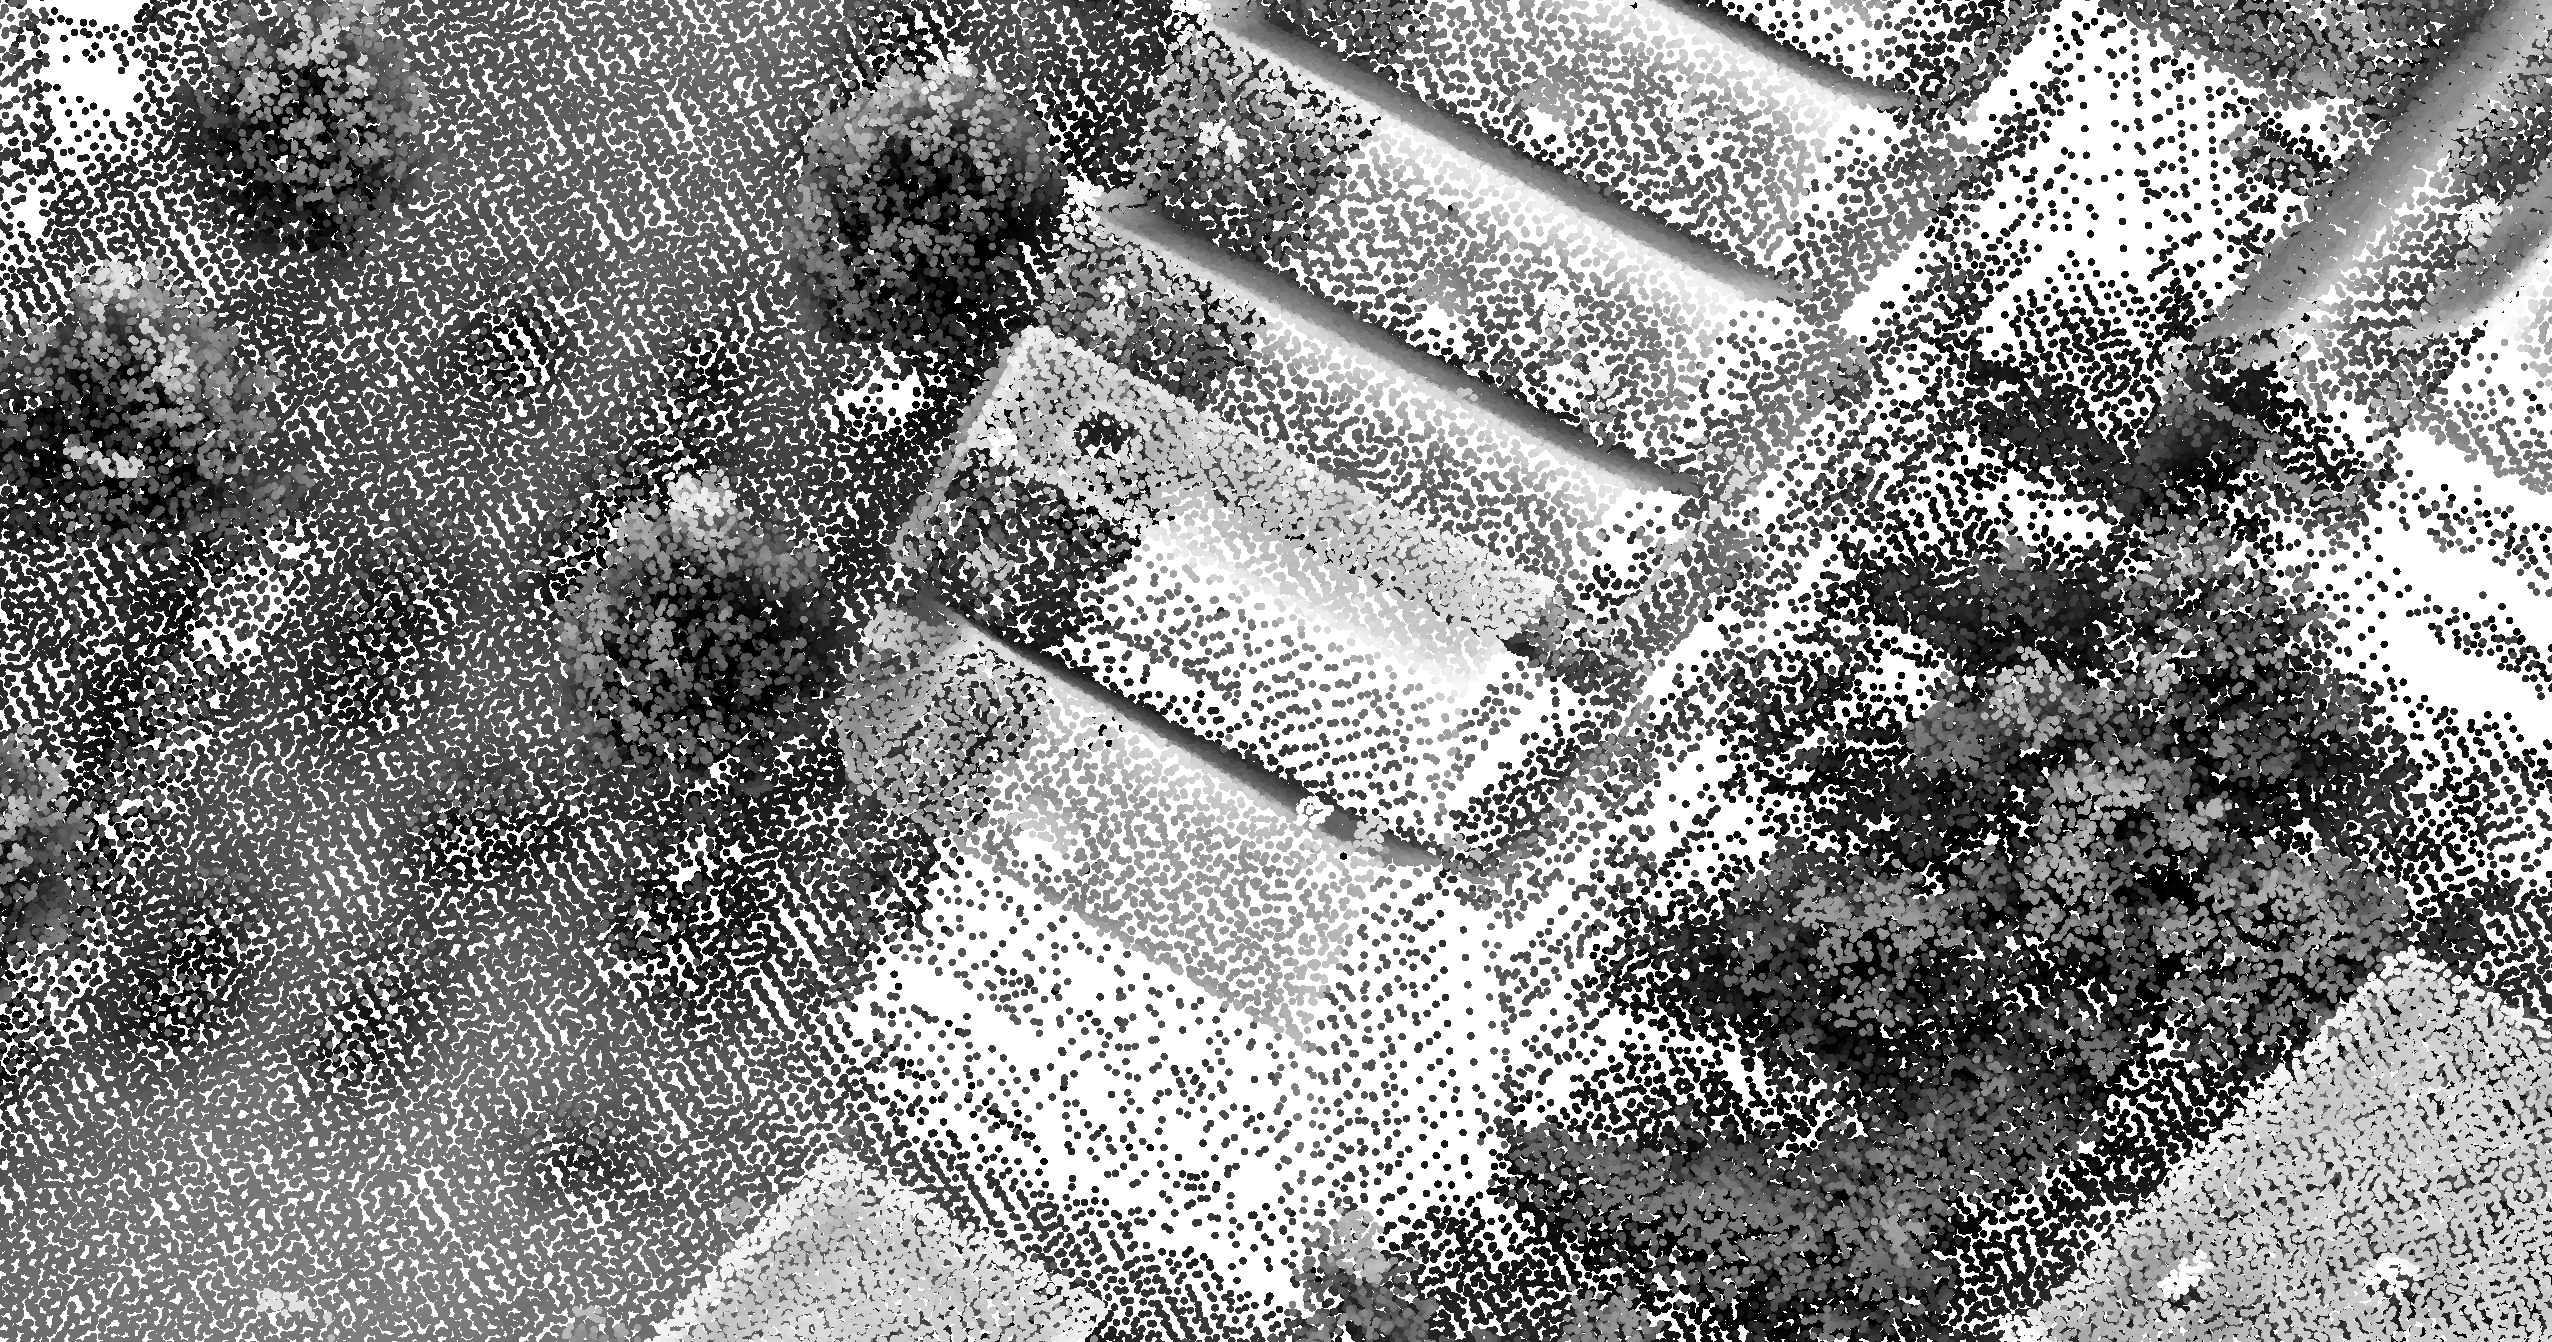
\includegraphics[width=\textwidth]{figs/rdam16_d.png}
		\subcaption{City of Rotterdam (2016)}\label{fig:pcd:rdam16}
	\end{subfigure}
	\caption{Several lidar point clouds for the same area in the city of Rotterdam. Point distribution and occlusion effects vary.}%
\label{fig:pcd}
\end{figure*}

\subsubsection{Material properties}
Depending on material properties of a target surface, signals may be reflected in a way that makes it impossible to compute the correct distance. 
Surfaces that act like a mirror are especially problematic, Figure~\ref{fig:lidarAcquisitionConditions:b} illustrates this. 
\begin{marginfigure}
	\centering
	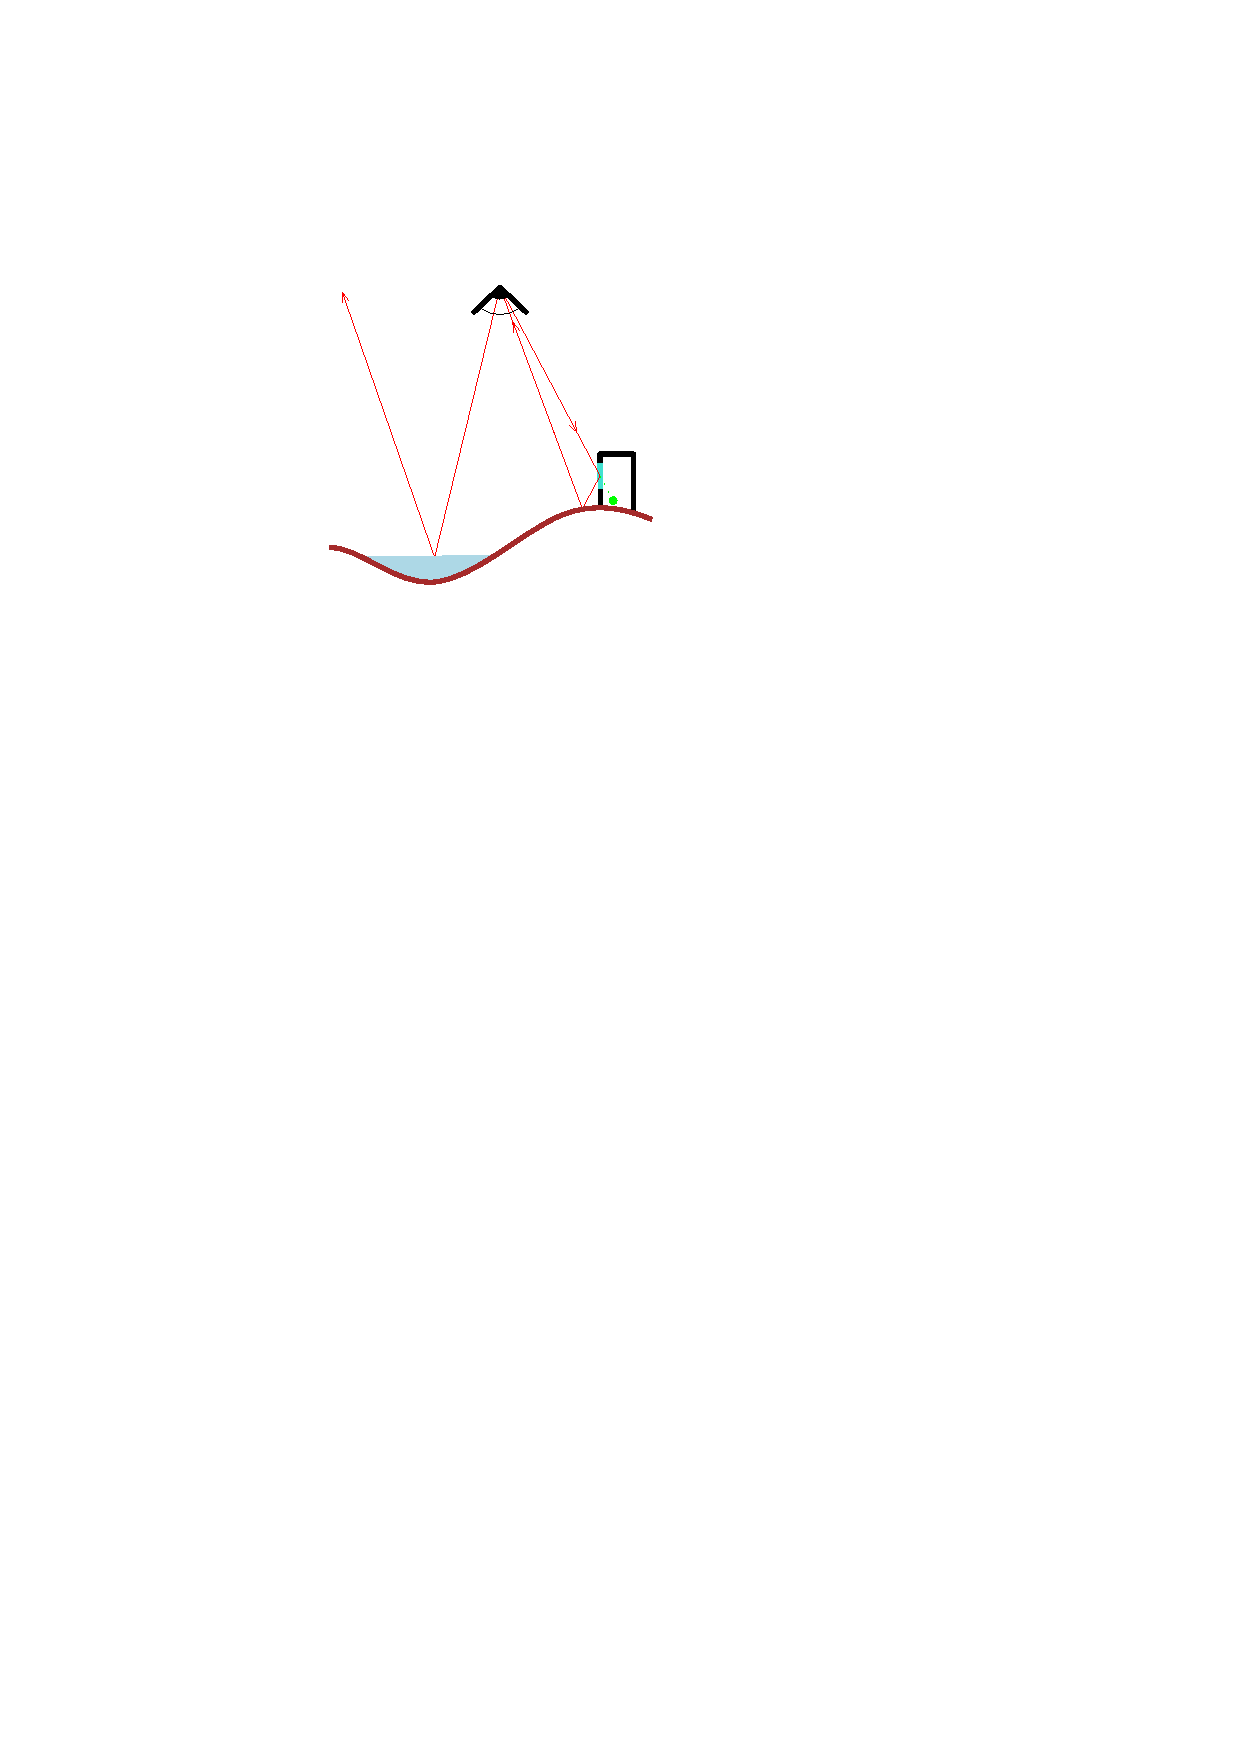
\includegraphics[width=\textwidth,page=1]{figs/lidarAcq.pdf}
	\caption{Reflection and multi-path}%
	\label{fig:lidarAcquisitionConditions:b}
\end{marginfigure}
First, it may happen that a pulse is reflected away from the sensor, \eg\ from a water surface, resulting in no distance measurement for that pulse. 
Or, in the case of photogrammetry, we will observe a different reflection in each image which heavily distorts the matching process, sometimes resulting in extreme outliers for water surfaces.  
In some cases, and only for active sensors, the reflected pulse does make its way back to the sensor, see for example the right half of Figure~\ref{fig:lidarAcquisitionConditions:b}. 
However, it will have travelled a longer distance than it should have and the scanner only knows in which direction it emitted the pulse. 
This effect is called \emph{multi-path} and the result is that points are measured at a distance that is too long and therefore they show up below the ground surface in the point cloud (see Figure~\ref{fig:outliers}).  
\begin{figure}
	\centering
	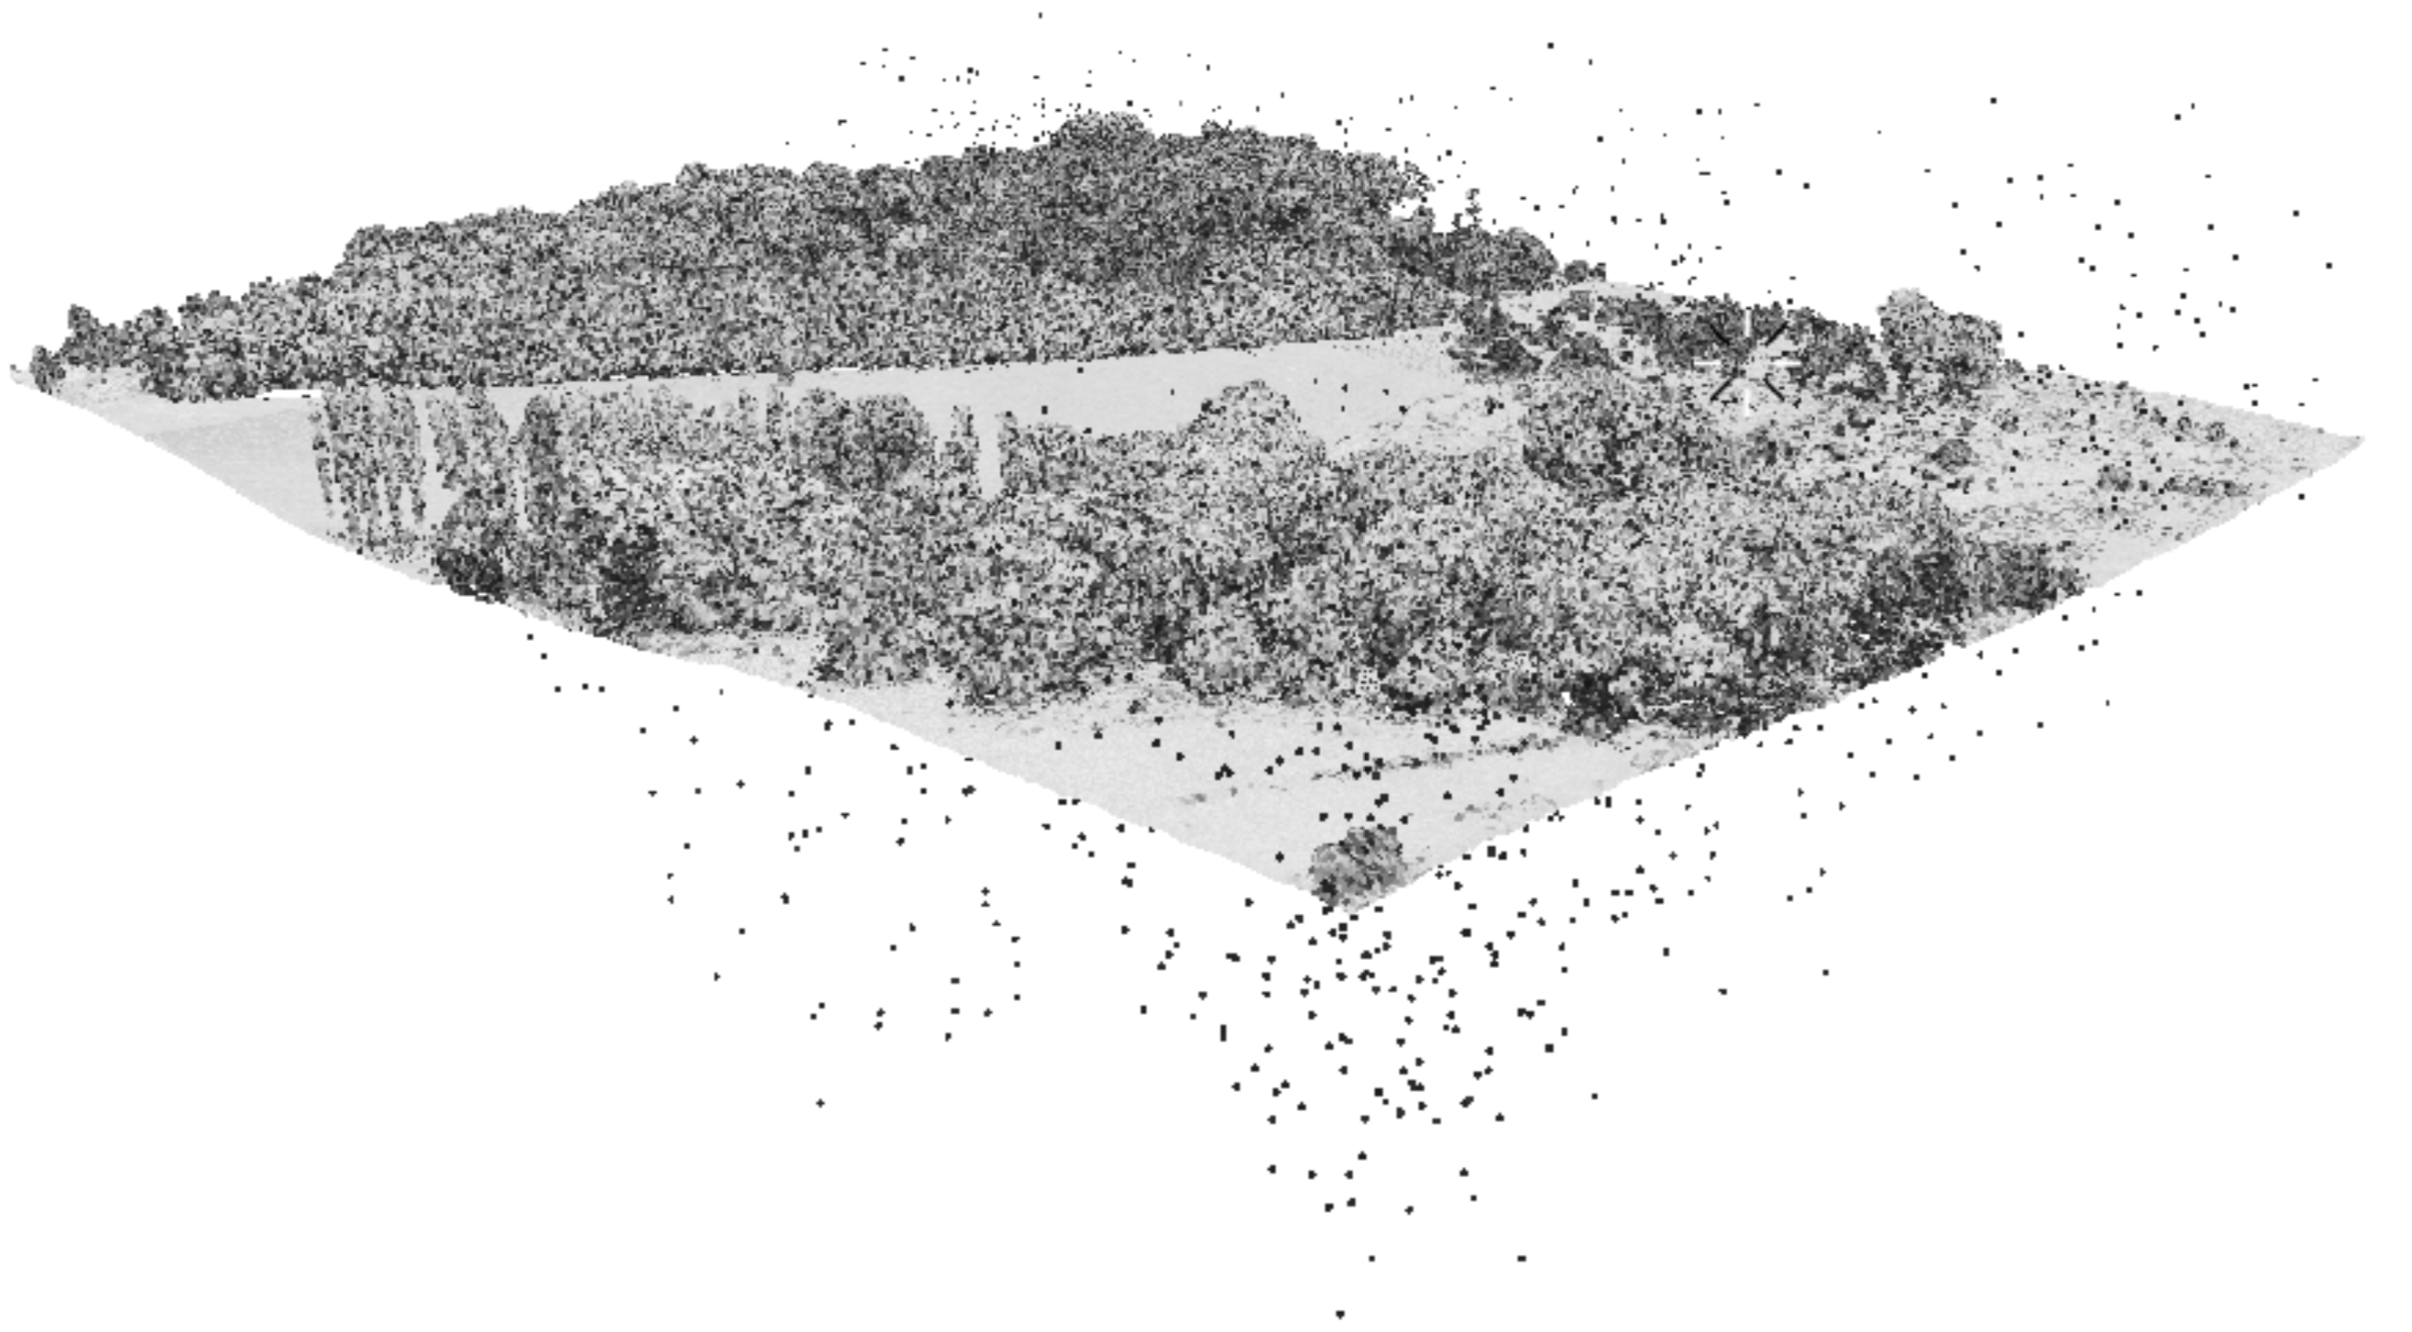
\includegraphics[width=\textwidth]{figs/outliers.png}
	\caption{Outliers, below and above the ground, in a lidar point cloud dataset.}%
\label{fig:outliers}
\end{figure}

Photogrammetry suffers from a few other problems as well, such as surfaces that have a homogeneous texture that make it impossible to find distinguishing features that can be used for matching. 
This may also happen in poor lightning conditions, for example in the shadow parts of an image.
%no texture (shadow), multi-path, complete absorption lightning conditions: shadow poor matching

\subsubsection{Moving objects}
An example of moving objects are flocks of birds flying in front of the scanner. These can cause outliers high above the ground, as illustrated in Figure~\ref{fig:outliers}.


\subsection{Processing}
It is common to perform some kind of process after acquisition in order to fix errors caused by the reasons mentioned above. 
In most cases such processes are largely successful. 
For instance, one can attempt to fill the void regions, sometimes referred to as \emph{no-data} regions, that are for instance due to pools of rainwater or occlusion, using an interpolation method (Figure~\ref{fig:voidfill}).
\begin{figure*}
	\centering
	\begin{subfigure}{0.45\linewidth}
		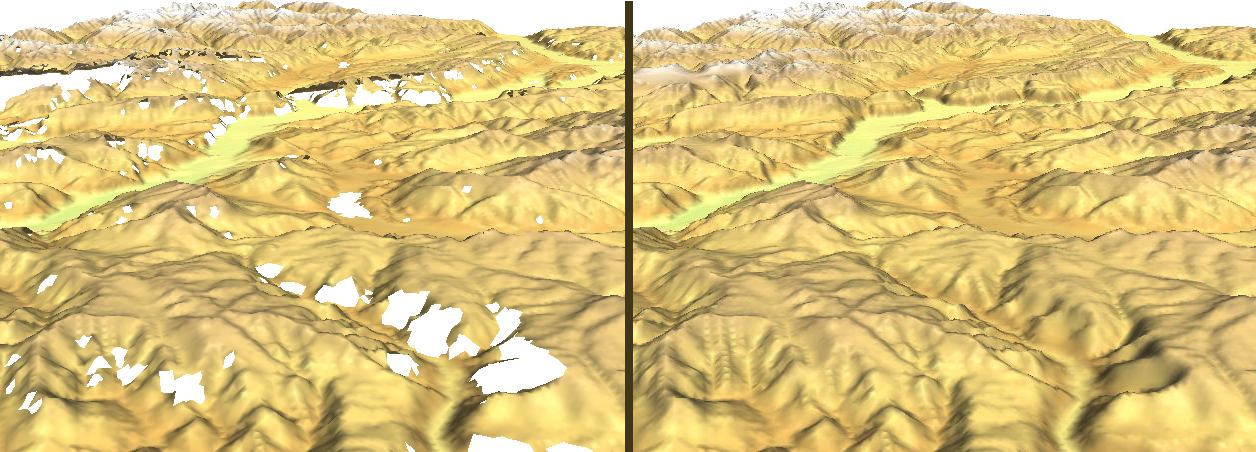
\includegraphics[width=\textwidth]{figs/srtm_trento_voidfill.png}
		\subcaption{Void-filling through interpolation in SRTM data}\label{fig:voidfill}
	\end{subfigure}
	\quad
	\begin{subfigure}{0.45\linewidth}
		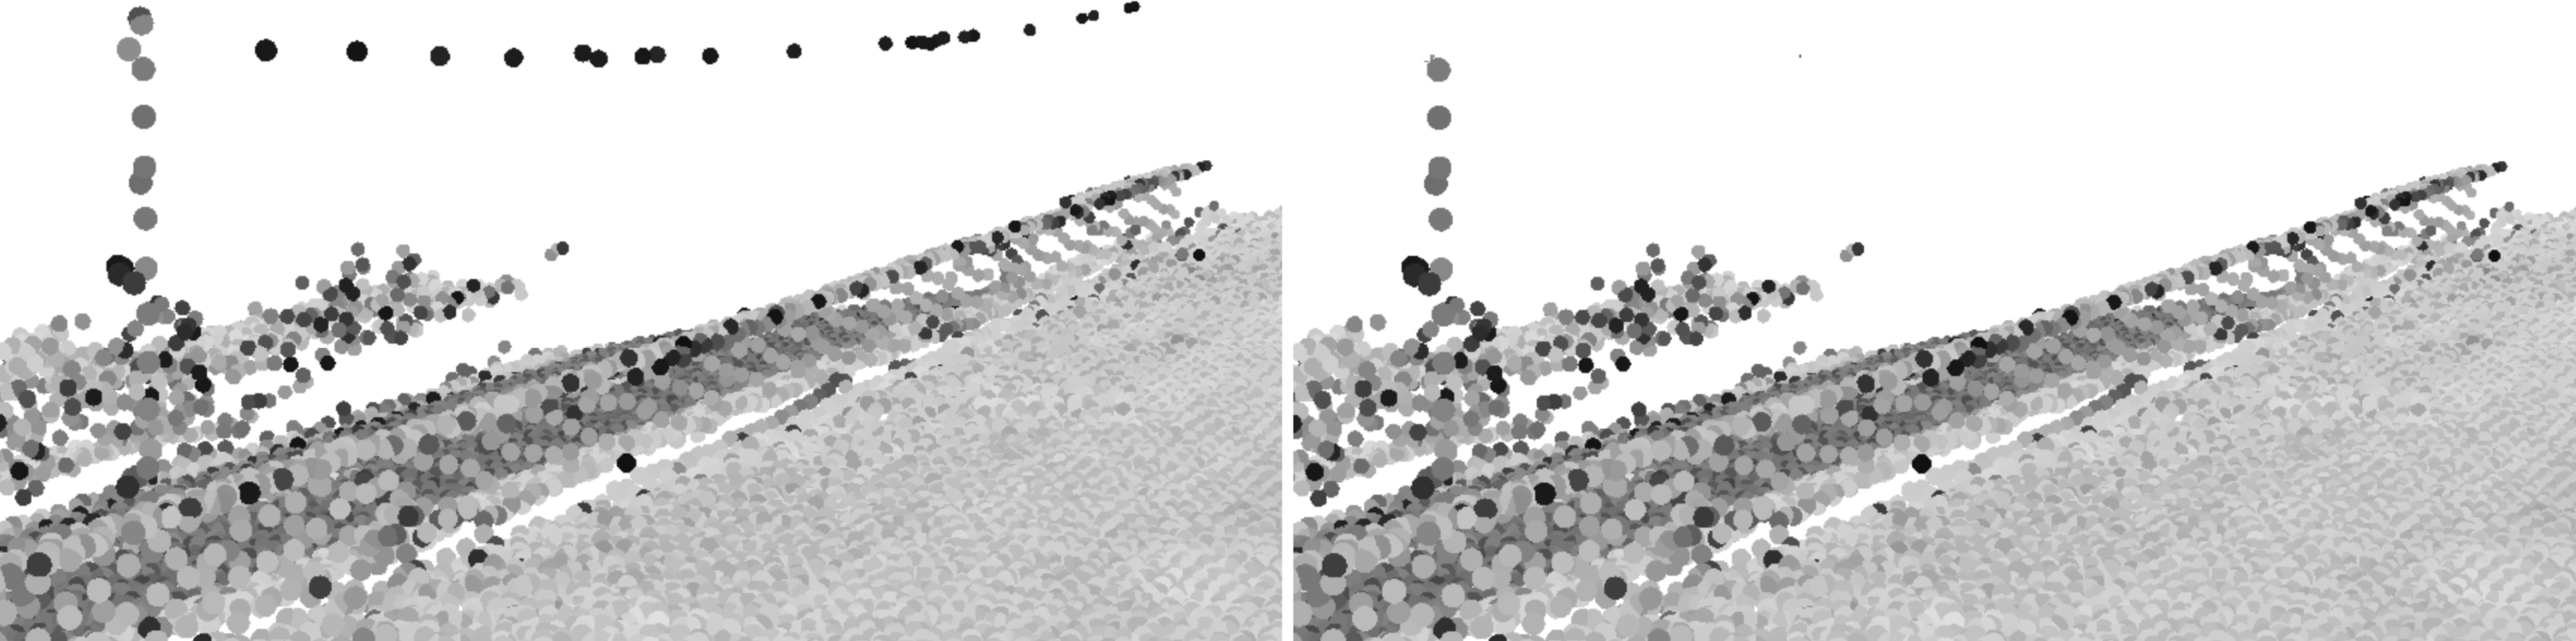
\includegraphics[width=\textwidth]{figs/ourlier-detection-wrong.png}
		\subcaption{Good points, \ie\ those on the power line, may be removed during outlier detection}\label{fig:outlier-wrong}
	\end{subfigure}
	\caption{Post-processing aimed at correcting artefacts. Before processing (left) and after processing (right).}%
	\label{fig:processing}
\end{figure*}
Or, one can attempt to detect and remove outliers caused \eg\ by multi-path effects or flocks of birds\sidenote{This is a topic of Chapter~\ref{chap:pcprocessing}}. 
However, while the intention is always to reduce the number and severity of artefacts, these processes sometimes introduce distortions of their own.
For example, an outlier detection algorithm may remove `good' points if they look the same as outliers to the outlier detection algorithm (see \eg\ Figure~\ref{fig:outlier-wrong}).
And void-filling is only effective if the void area is not too large, since interpolation methods always assume there is sufficient neighbourhood information to work with\sidenote{Chapters~\ref{chap:interpol} and~\ref{chap:kriging} explore the topic of spatial interpolation in detail.}.


%%
\begin{kaobox-toread}[frametitle=\faExternalLink\ To read or to watch]
This is a paper that compares lidar and photogrammetry derived point clouds for the generation of a DEM\@. It shows that even when artefacts seem to be under control, both techniques may measure different elevations 

\fullcite{Ressl16}
\textbf{PDF:} \url{https://3d.bk.tudelft.nl/courses/geo1015/data/others/Ressl16.pdf}
\end{kaobox-toread}

%For instance, an outlier filter 
%misclassified points, smoothing effects in DIM

% Difficulties in automated DTM generation
% - Homogeneous areas and repeating structures;
% - No distinct peak or multiple peaks of the similarity measures
% - Areas occluded in one image
% - No correspondence exists;
% - Steep sloped surfaces
% - Geometric difference between template and match window;
% - Discontinuities and break-lines
% - No correspondence or geometric difference;
% - Non-lambertian surfaces
% - Radiometric difference between template and match window;
% - Moving objects
% - correct correspondence, incorrect elevation

% strip misalignment
% occlusion/geometry of target surface vs scanning position, density of points
% season- leaves on trees
% lightning conditions/shadow for photogrammetry
% surface material - reflactance, absorbance, multi echo, multiple returns


%few words about sensor fusion?


%%%
%
\section{Notes and comments}
If you would like to learn more about how a lidar scanner works, the chapter from \citet{Chazette16} is recommended.
More details on InSAR can be found in the manual from \citet{ESA07}.

\citet{Reuter09} give an elaborate overview of the processing that needs to be done to derive a high quality (raster) DTM from raw elevation measurements.

% fixing dem artefacts: https://www.sciencedirect.com/science/article/pii/S0166248108000044

%%%%%%%%%%%%%%%%%%%%
%
\section{Exercises}

\begin{enumerate}
	\item Name three differences between point cloud acquisition with lidar and with photogrammetry.
	\item Explain what the time-of-flight principle entails.
	\item How can you minimise occlusion effects in a point cloud during acquisition?
	\item Why does positioning, using for instance GPS, play such an important role in acquisition?
\end{enumerate}

%!TEX root = ../terrainbook.tex

\graphicspath{{dtvd/}}


\newcommand{\Orient}{O\textsc{rientation}\xspace}
\newcommand{\walk}{W\textsc{alk}\xspace}
\newcommand{\Incircle}{I\textsc{n}C\textsc{ircle}\xspace}

\chapter{Triangulations \& Voronoi diagrams}%
\label{chap:dtvd}

% TODO : introduction to the chapter: DT and VD are fundamental structures in terrains, both for representation but also for processing (interpolation and many other operations with terrains and point clouds)


\section{The Voronoi Diagram}

Let $S$ be a set of points in $\mathbb{R}^2$ (the two-dimensional Euclidean space). 
The Voronoi cell of a point $p \in S$, defined $\mathcal{V}_{p}$, is the set of points $x \in \mathbb{R}^2$ that are closer to $p$ than to any other point in $S$; that is:
\begin{equation}
\mathcal{V}_p = \{x \in \mathbb{R}^{2} \ | \ \|x-p\| \, \leq \, \|x-q\|, \ \forall \, q \in S \}. 
\end{equation}
The union of the Voronoi cells of all generating points $p \in S$ form the Voronoi diagram of $S$, defined VD($S$). 
If $S$ contains only two points $p$ and $q$, then VD($S$) is formed by a single line defined by all the points $x \in \mathbb{R}^2$ that are equidistant from $p$ and $q$. 
This line is the perpendicular bisector of the line segment from $p$ to $q$, and splits the plane into two half-planes. 
$\mathcal{V}_p$ is formed by the half-plane containing $p$, and $\mathcal{V}_q$ by the one containing $q$. 
As shown in Figure~\ref{fig:halfspaces}a,
\begin{figure}
  \centering
  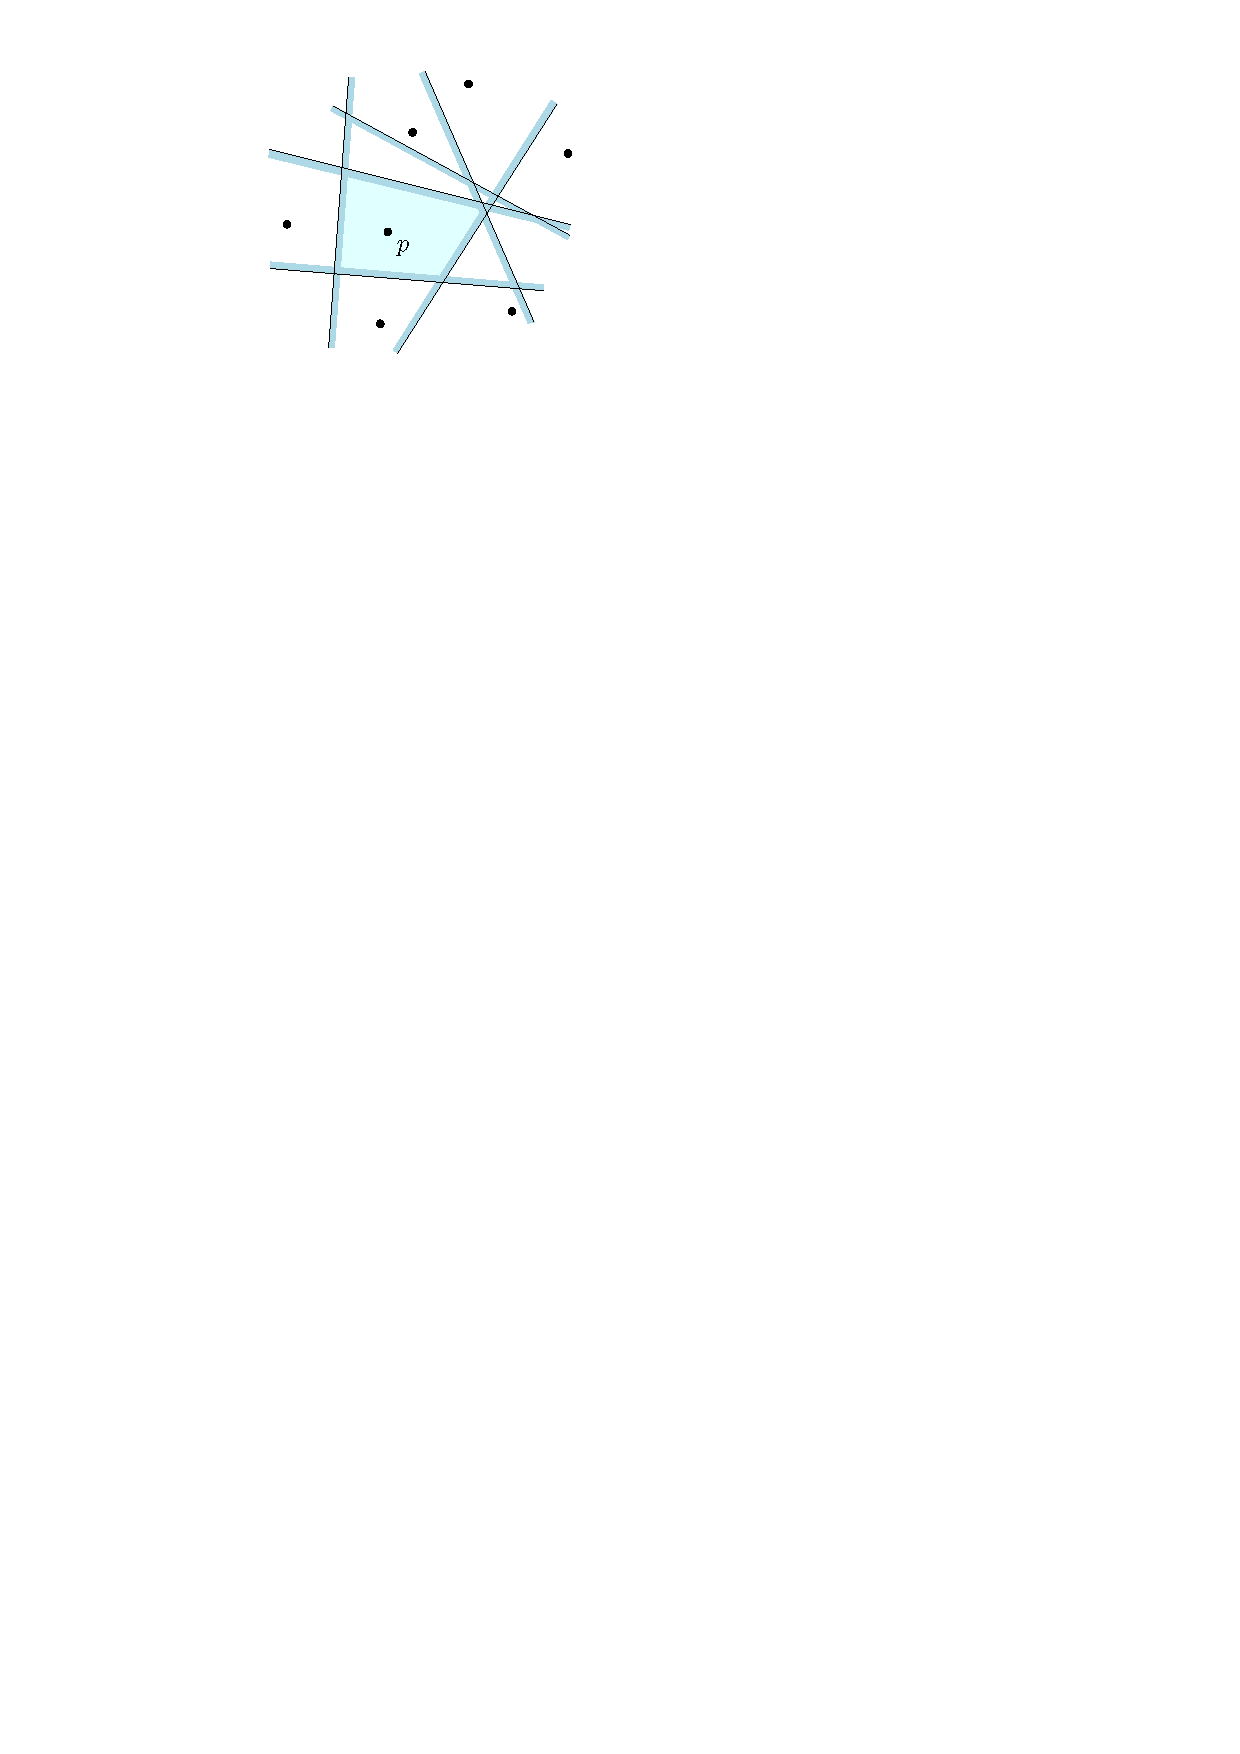
\includegraphics[width=0.6\textwidth]{figs/halfspaces}
  \caption{\textbf{(a)} The Voronoi cell $\mathcal{V}_p$ is formed by the intersection of all the half-planes between $p$ and the other points. \textbf{(b)} The VD for a set $S$ of points in the plane (the black points). The Voronoi vertices (white points) are located at the centre of the circle passing through three points in $S$, provided that this circle contains no other points in $S$ in its interior.} 
\label{fig:halfspaces}
\end{figure}
when $S$ contains more than two points (let us say it contains $n$ points), the Voronoi cell of a given point $p \in S$ is obtained by the intersection of $n-1$ half-planes defined by $p$ and the other points $q \in S$. 
That means that $\mathcal{V}_{p}$ is always convex. 
Notice also that every point $x \in \mathbb{R}^2$ has at least one nearest point in $S$, which means that VD($S$) covers the entire space.

%

As shown in Figure~\ref{fig:halfspaces}b, the VD of a set $S$ of points in $\mathbb{R}^2$ is a planar graph. 
Its edges are the perpendicular bisectors of the line segments of pairs of points in $S$, and its vertices are located at the centres of the circles passing through three points in $S$. 
The VD in $\mathbb{R}^2$ can also be seen as a two-dimensional cell complex where each 2-cell is a (convex) polygon (see Figure~\ref{fig:vd2d}). 
\begin{figure}
  \centering
  \includegraphics[page=3,width=0.6\textwidth]{figs/vd2d}
  \caption{VD of a set of points in the plane (clipped by a box). The point $p$ (whose Voronoi cell is dark grey) has seven neighbouring cells (light grey).} 
\label{fig:vd2d}
\end{figure}
Two Voronoi cells, $\mathcal{V}_{p}$ and $\mathcal{V}_{q}$, lie on the opposite sides of the perpendicular bisector separating the points $p$ and $q$. 

%

The VD has many interesting properties, what follows is a list of the most relevant properties in the context of this course.
\begin{description}
  \item[Size:] if $S$ has $n$ points, then VD($S$) has exactly $n$ Voronoi cells since there is a one-to-one mapping between the points and the cells.
  \item[Voronoi vertices:] a Voronoi vertex is equidistant from 3 data points. Observe for instance in Figure~\ref{fig:halfspaces}b that the Voronoi vertices are at the centre of circles.
  \item[Voronoi edges:] a Voronoi edge is equidistant from 2 points.
  \item[Convex hull:] let $S$ be a set of points in $\mathbb{R}^2$, and $p$ one of its points. $\mathcal{V}_{p}$ is unbounded if $p$ bounds conv($S$). Otherwise, $\mathcal{V}_{p}$ is the convex hull of its Voronoi vertices. Observe that in Figure~\ref{fig:halfspaces}b, only the point in the middle has a bounded Voronoi cell.
\end{description}
  

%%%
%
\section{The Delaunay Triangulation}
\label{sec:dt_definition}

Let $\mathcal{D}$ be the VD of a set $S$ of points in $\mathbb{R}^2$. 
Since VD($S$) is a planar graph, it has a dual graph, and let $\mathcal{T}$ be this dual graph obtained by drawing straight edges between two points $p,q \in S$ if and only if $\mathcal{V}_{p}$ and $\mathcal{V}_{q}$ are adjacent in $\mathcal{D}$. 
Because the vertices in $\mathcal{D}$ are of degree 3 (3 edges connected to it), the graph $\mathcal{T}$ is a triangulation. 
$\mathcal{T}$ is actually called the Delaunay triangulation (DT) of $S$, and, as shown in Figure~\ref{fig:dt2da}, 
\begin{figure}
  \centering
  \begin{subfigure}[b]{0.45\linewidth}
    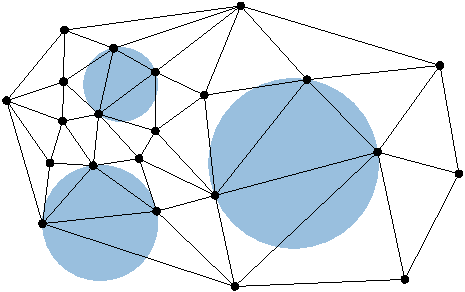
\includegraphics[width=\textwidth]{figs/dt2d_2}
    \caption{}\label{fig:dt2da}
  \end{subfigure}%
  \qquad
  \begin{subfigure}[b]{0.3\linewidth}
    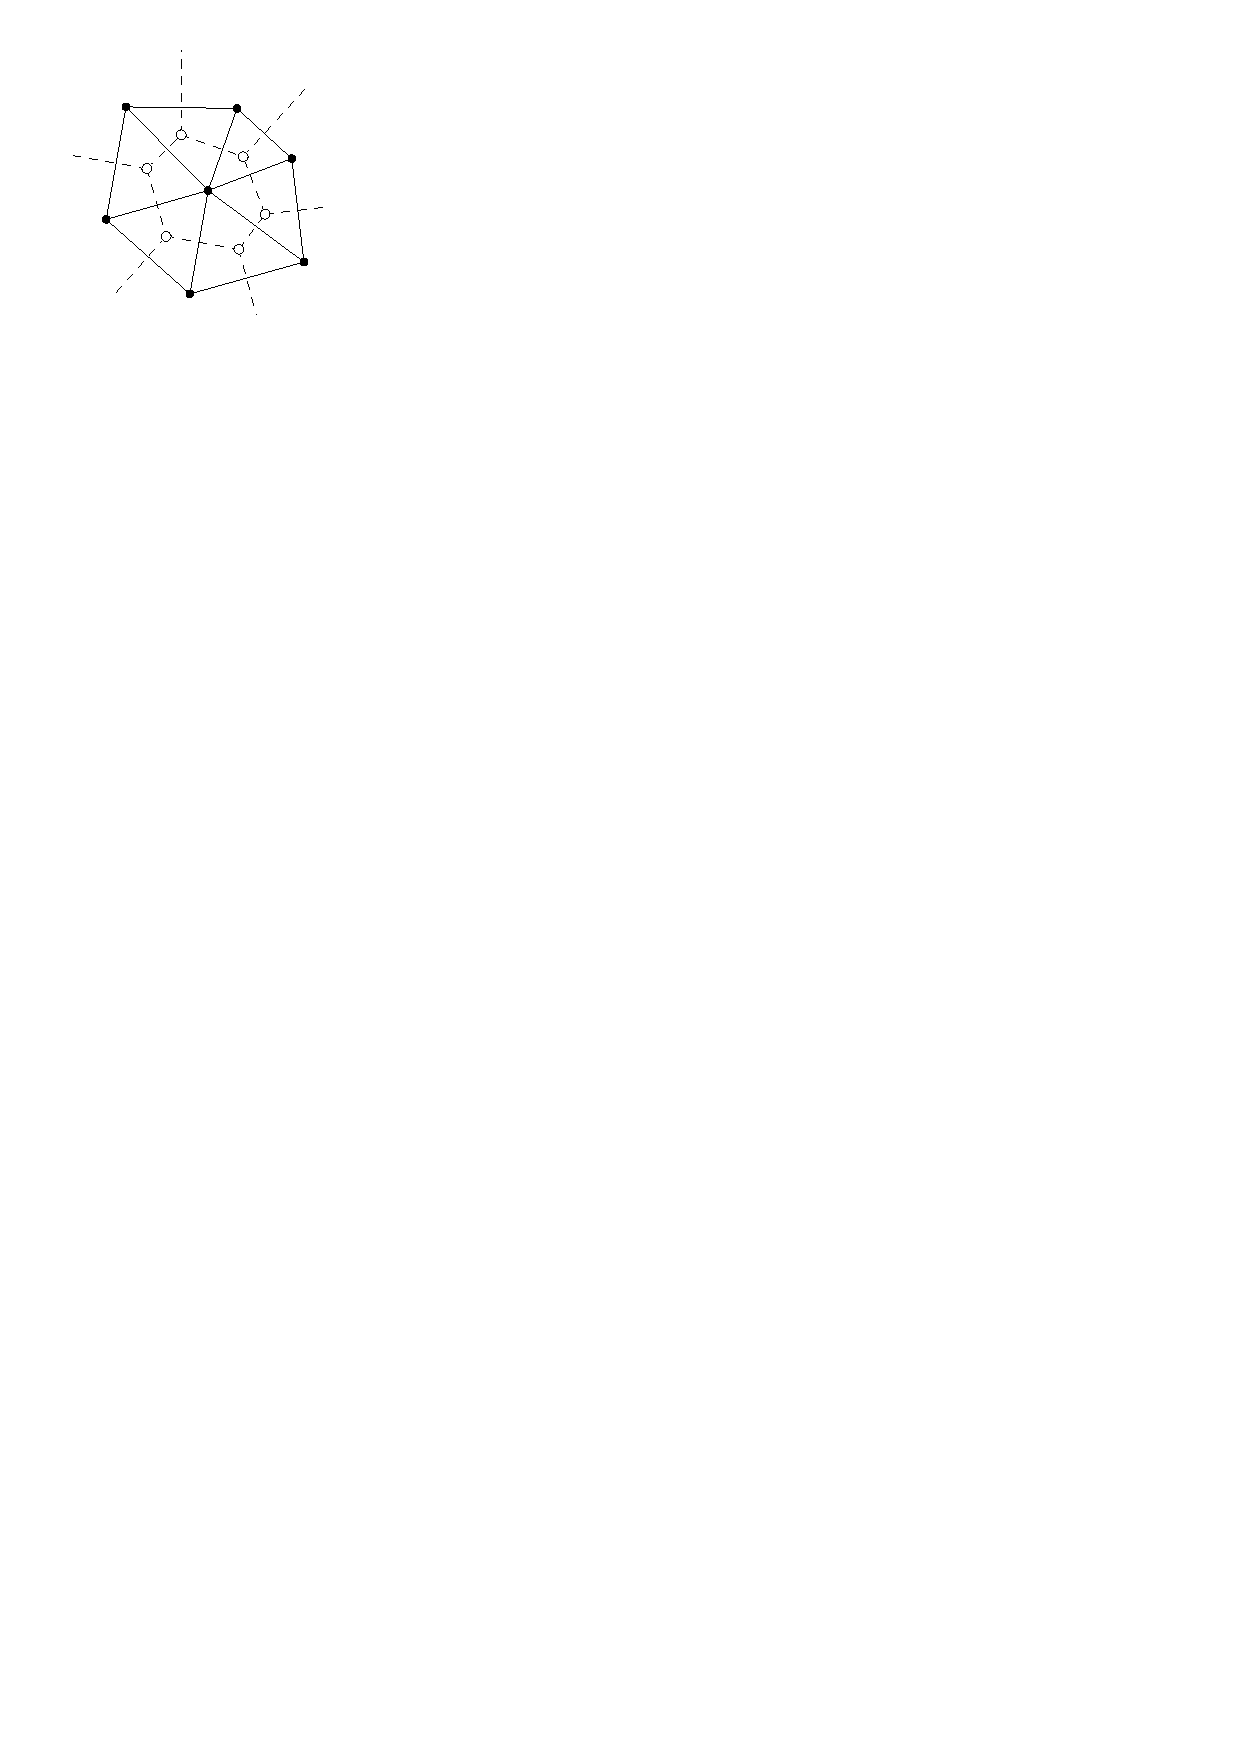
\includegraphics[width=\textwidth]{figs/duality_2d}
    \caption{}\label{fig:dt2db}
  \end{subfigure}%
  \caption{\textbf{(a)} The DT of a set of points in the plane (same point set as Figure~\ref{fig:vd2d}). \textbf{(b)} Both the DT (black lines) and the VD (dashed lines) of a set of points in the plane.}
\label{fig:dt2d}
\end{figure}
partitions the plane into triangles---where the vertices of the triangles are the points in $S$ generating each Voronoi cell---that satisfy the \emph{empty circumcircle} test (a circle is said to be \emph{empty} when no points are in its interior). 
If $S$ is in general position, then DT($S$) is unique.

%
\subsection{Convex Hull}
The DT of a set $S$ of points subdivides completely conv($S$), \ie\ the union of all the triangles in DT($S$) is conv($S$).

Let $S$ be a set of points in $\mathbb{R}^2$, the \emph{convex hull} of $S$, denoted conv($S$), is the minimal convex set containing $S$. 
It is best understood with the elastic band analogy: imagine each point in $\mathbb{R}^2$ being a nail sticking out of the plane, and a rubber band stretched to contain all the nails, as shown in Figure~\ref{fig:convex_hull}. 
\begin{figure}
  \centering
  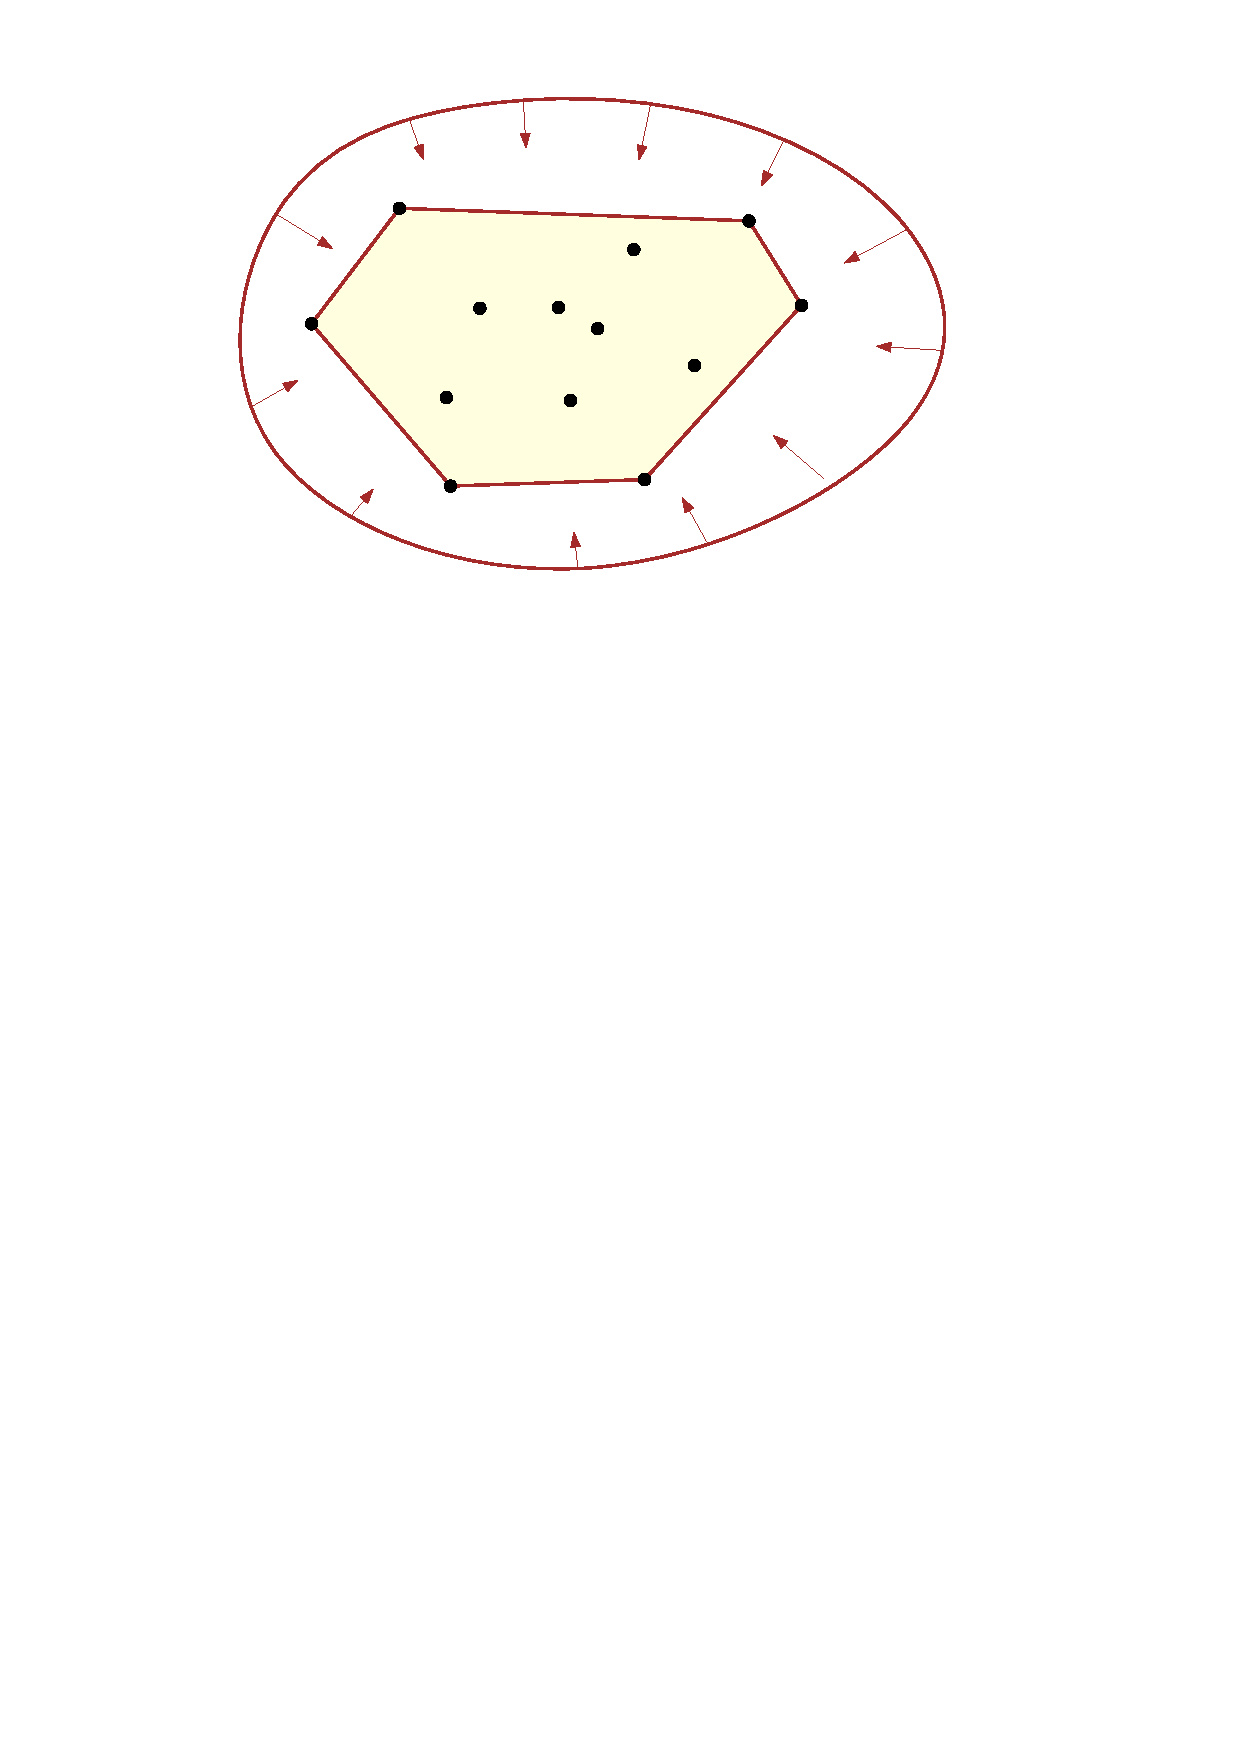
\includegraphics[width=0.35\textwidth]{figs/convex_hull}
  \caption{The convex hull of a set of points in $\mathbb{R}^2$.} 
\label{fig:convex_hull}
\end{figure}
When released, the rubber band will assume the shape of the convex hull of the nails. 
Notice that conv($S$) is not only formed by the edges connecting the points (the rubber band), but all the points of $\mathbb{R}^2$ that are contained within these edges (thus the whole polygon).


%
\subsection{Local Optimality}
Let $\mathcal{T}$ be a triangulation of $S$ in $\mathbb{R}^2$. 
An edge $\sigma$ is said to be \emph{locally} Delaunay if it either:
\begin{description}
  \item[(i)] belongs to only one triangle, and thus bounds conv($S$), or
  \item[(ii)] belongs to two triangles $\tau_a$ and $\tau_b$, formed by the vertices of $\sigma$ and respectively the vertices $p$ and $p$, and $p$ is outside of the circumcircle of $\tau_a$. 
\end{description}
The second case is illustrated in Figure~\ref{fig:local}: the triangles $abd$ and $bcd$ are Delaunay, and thus is the edge $bd$; the edge $ac$ is not Delaunay.
\begin{figure}
  \centering
  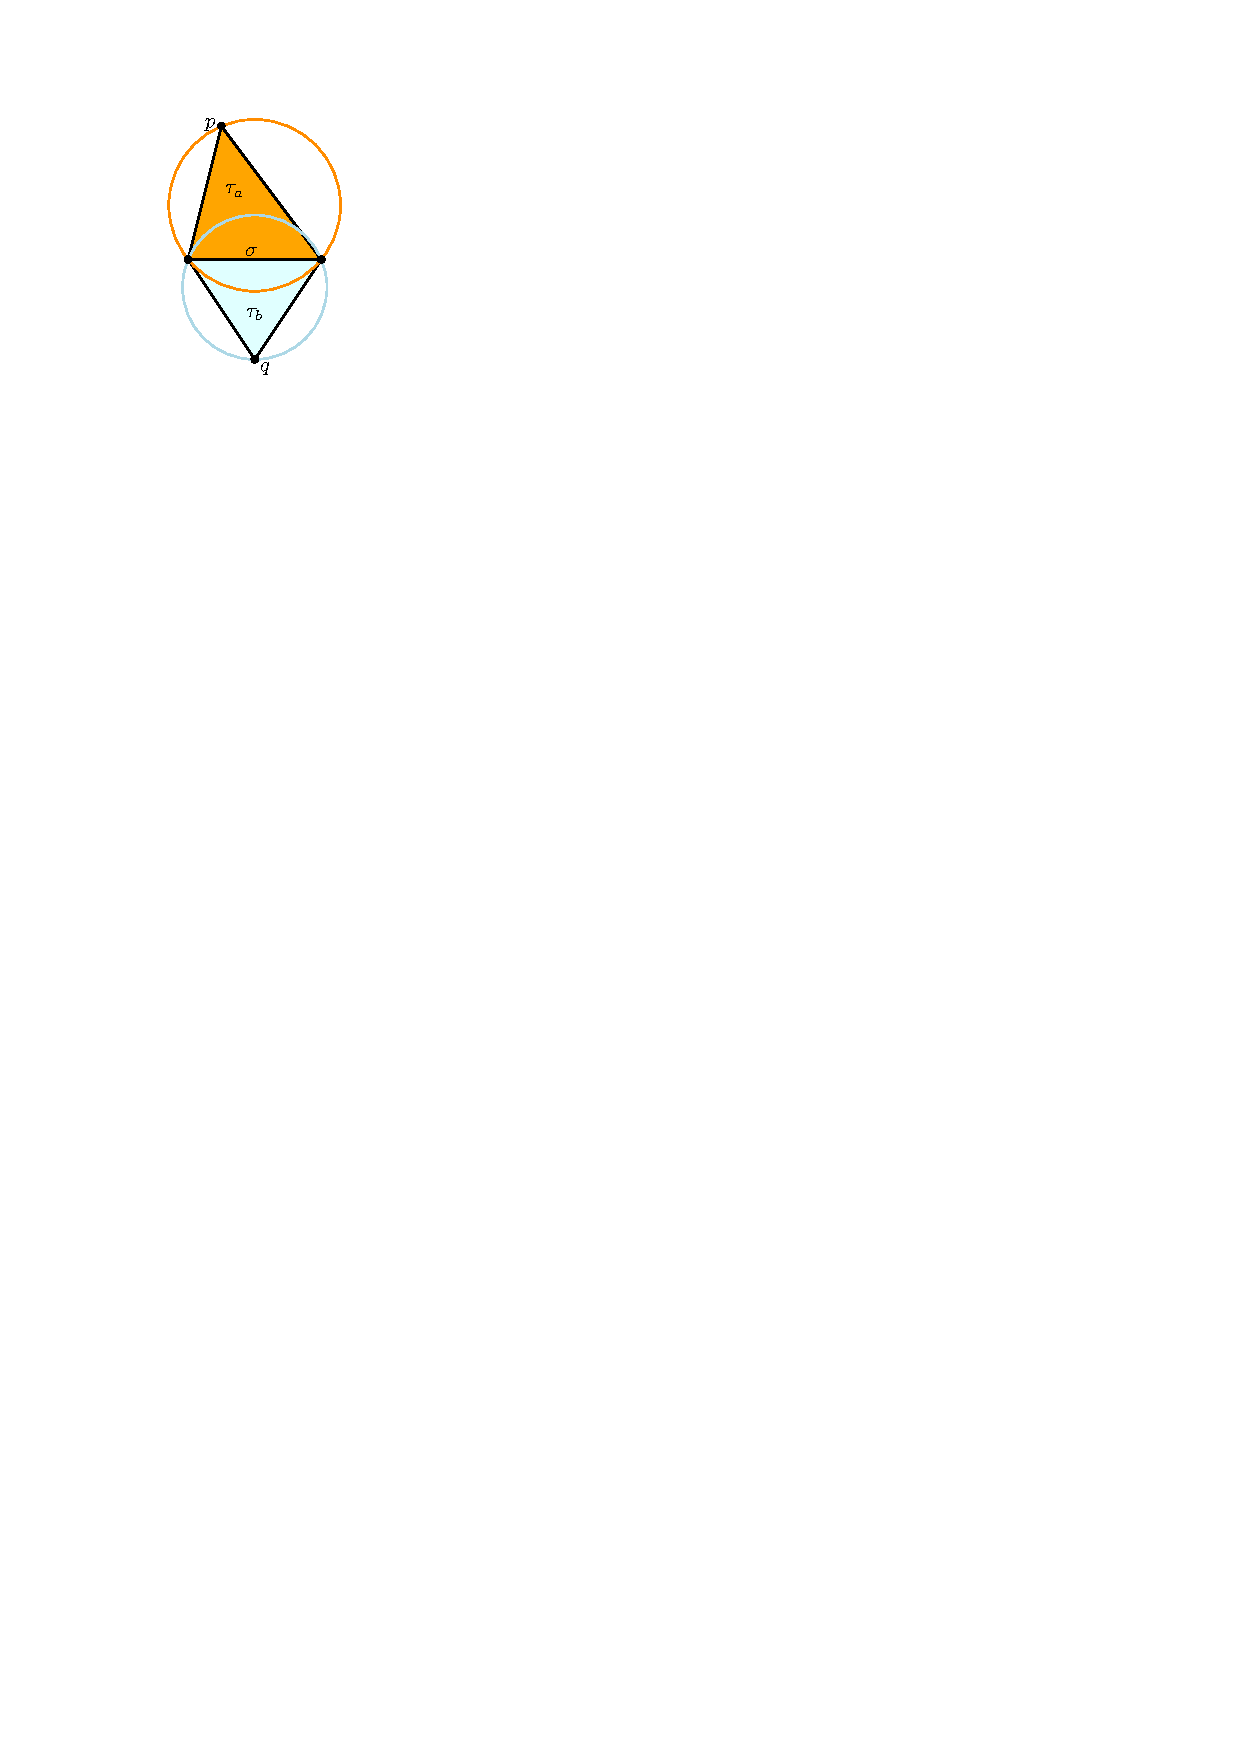
\includegraphics[width=0.7\textwidth]{figs/local}
  \caption{Only one configuration is Delaunay (the left one).} 
\label{fig:local}
\end{figure}
In an arbitrary triangulation, not every edge that is locally Delaunay is necessarily a edge of DT($S$), but local optimality implies globally optimality in the case of the DT:
\begin{quote}
  Let $\mathcal{T}$ be a triangulation of a point set $S$ in $\mathbb{R}^2$. If every edge of $\mathcal{T}$ is locally Delaunay, then $\mathcal{T}$ is the Delaunay triangulation of $S$.
\end{quote}
This has serious implications as the DT---and its dual---are locally modifiable, \ie\ we can theoretically insert, delete or move a points in $S$ without recomputing DT($S$) from scratch.


%%%
%
\subsection{Angle Optimality}
The DT in two dimensions has a very important property that is useful in applications such as finite element meshing or interpolation: the \emph{max-min angle optimality}. Among all the possible triangulations of a set $S$ of points in $\mathbb{R}^2$, DT($S$) maximises the minimum angle (max-min property), and also minimises the maximum circumradii. 
In other words, it creates triangles that are as equilateral as possible. 
Notice here that maximising the minimum angle is not the same as minimising the maximum, and the DT only guarantees the former.


%%%
\subsection{Lifting on the paraboloid}
\label{sec:parabolic_lifting}

There exists a close relationship between DTs in $\mathbb{R}^{d}$ and convex polytopes in $\mathbb{R}^{d+1}$. 

Let $S$ be a set of points in $\mathbb{R}^{d}$, and let $x_{1}, x_{2}, \ldots , x_{d}$ be the coordinates axes. 
The parabolic lifting map projects each vertex $v(v_{x1}, v_{x2}, \ldots , v_{xd})$ to a vertex $v^{+}(v_{x1}, v_{x2}, \ldots , v_{xd}, v_{x1}^{2}+v_{x2}^{2}+\cdots+v_{xd}^{2})$ on the paraboloid of revolution in $\mathbb{R}^{d+1}$. 
The set of points thus obtained is denoted $S^{+}$. 
Observe that, for the two-dimensional case, the paraboloid in three dimensions defines a surface whose vertical cross sections are parabolas, and whose horizontal cross sections are circles; the same ideas are valid in higher dimensions. 

%

The relationship is the following: every facet (a $d$-dimensional simplex) of the lower envelope of conv($S^{+}$) projects to a $d$-simplex of the Delaunay triangulation of $S$. 
This is illustrated in Figure~\ref{fig:paraboloid} for the construction of the DT in $\mathbb{R}^{2}$. 
\begin{figure}
  \centering
  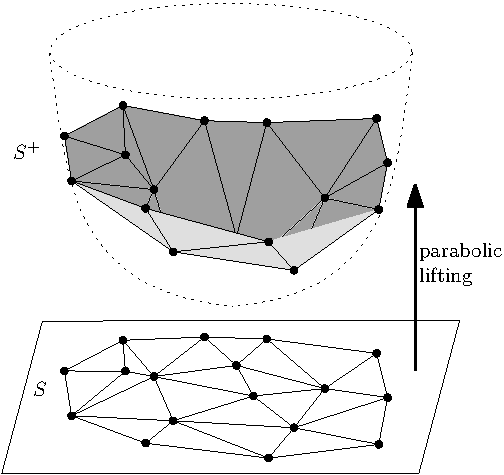
\includegraphics[width=0.4\textwidth]{figs/paraboloid}
  \caption{The parabolic lifting map for a set $S$ of points $\mathbb{R}^2$.}
\label{fig:paraboloid}
\end{figure}

%

In short, the construction of the $d$-dimensional DT can be transformed into the construction of the convex hull of the lifted set of points in ($d+1$) dimensions.
In practice, since it is easier to construct convex hulls (especially in higher dimensions, \ie\ 4+), the DT is often constructed with this method.




%%%
%
\subsection{Degeneracies}
\label{sec:degeneracies}

The previous definitions of the VD and the DT assumed that the set $S$ of points is in general position, \ie\ the distribution of points does not create any ambiguity in the two structures. 
For the VD/DT in $\mathbb{R}^{2}$, the degeneracies, or special cases, occur when 3 points lie on the same line and/or when 4 points are cocircular. 
For example, in two dimensions, when four or more points in $S$ are cocircular there is an ambiguity in the definition of DT($S$). 
As shown in Figure~\ref{fig:degeneracies},
\begin{figure}
  \centering
  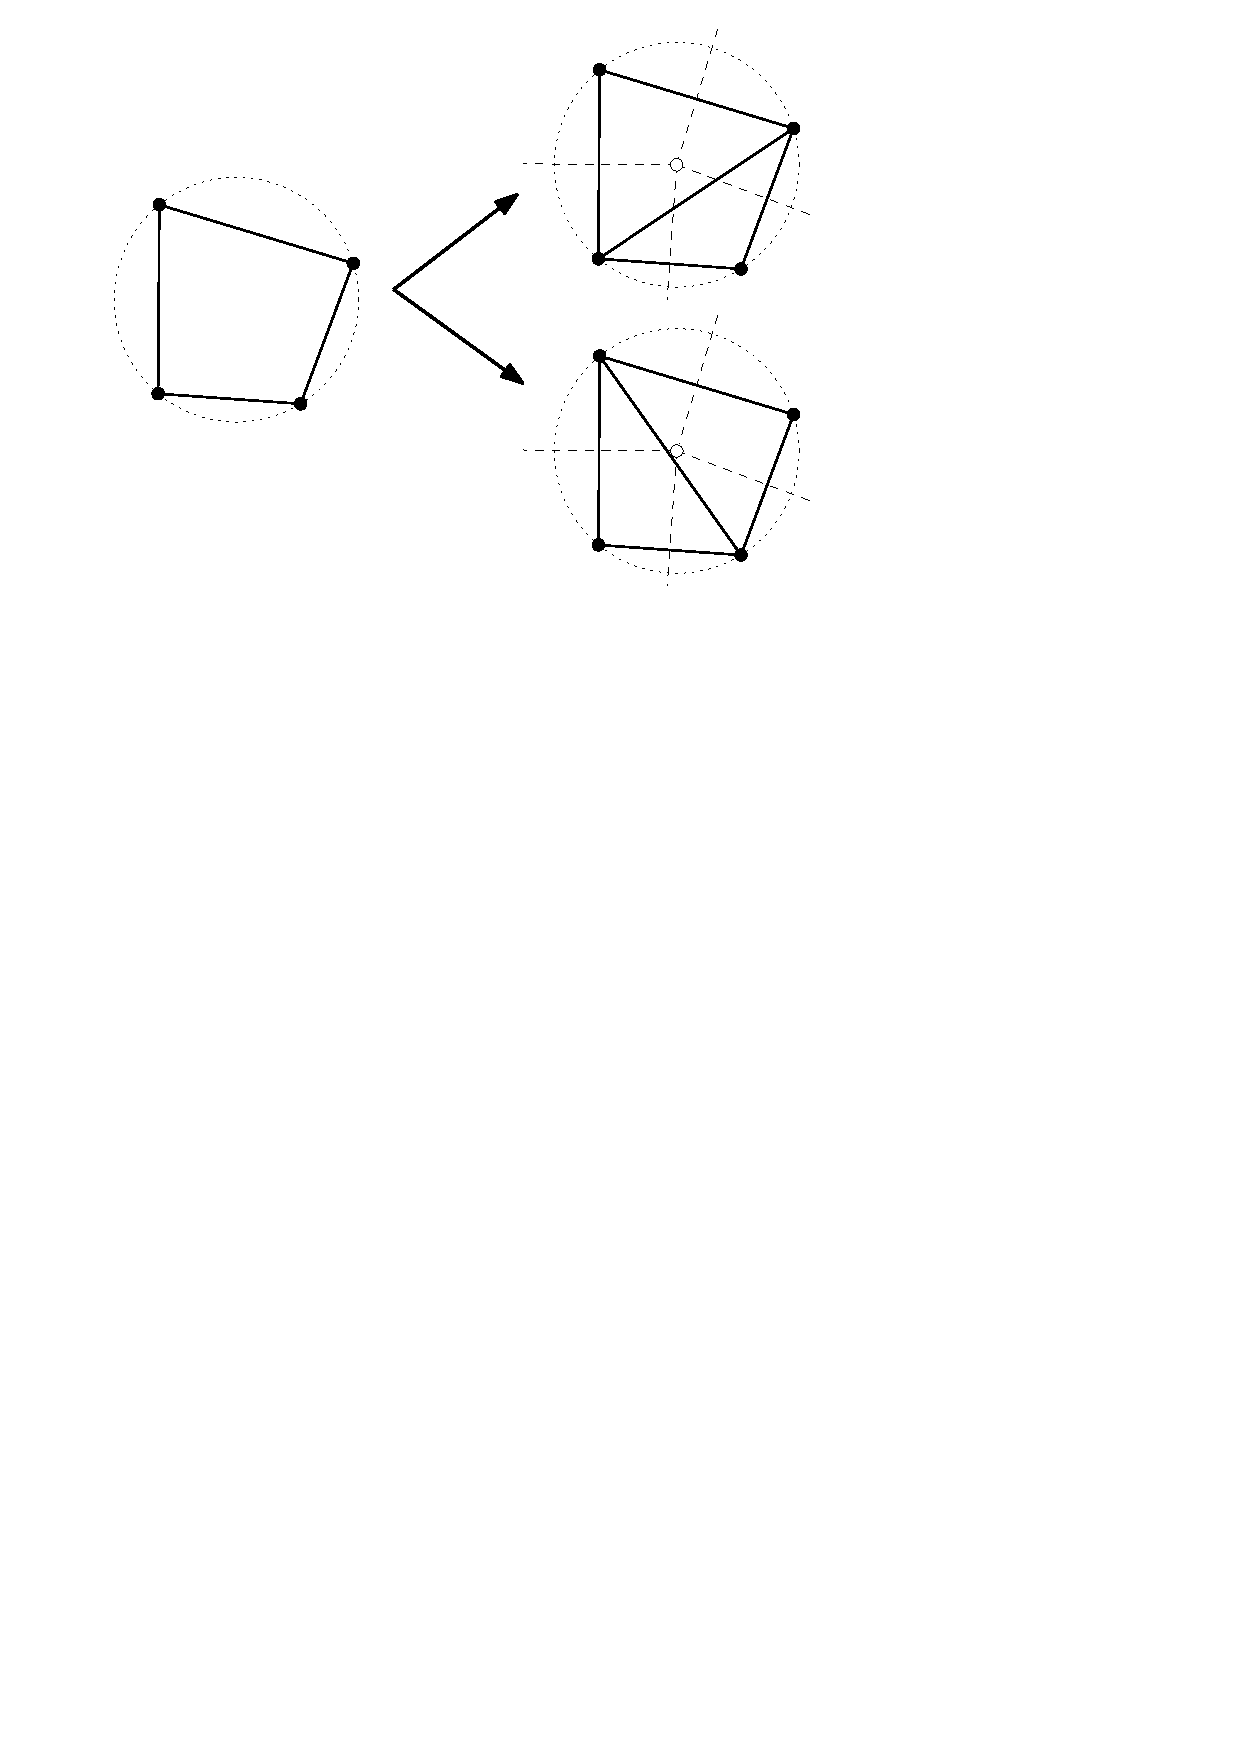
\includegraphics[width=0.4\textwidth]{figs/degeneracies}
  \caption{The DT for four cocircular points in two dimensions is not unique (but the VD is).}
\label{fig:degeneracies}
\end{figure}
the quadrilateral can be triangulated with two different diagonals, and an arbitrary choice must be made since both respect the Delaunay criterion (points should not be on the interior of a circumcircle, but more than three can lie directly on the circumcircle).

This implies that in the presence of four or more cocircular points, DT($S$) is not unique. 
Notice that even in the presence of cocircular points, VD($S$) is still unique, but it has different properties. 
For example, in Figure~\ref{fig:degeneracies}, the Voronoi vertex in the middle has degree 4 (remember that when $S$ is in general position, every vertex in VD($S$) has degree 3). 
When three or more points are collinear, DT($S$) and VD($S$) are unique, but problems with the implementation of the structures can arise.


%%%
%
\section{Duality between the DT and the VD}
\label{sec:duality}

Duality can have many different meanings in mathematics, but it always refers to the translation or mapping in a one-to-one fashion of concepts or structures. 
We use it in this course in the sense of the dual graph of a given graph. 
Let $G$ be a planar graph, as illustrated in Figure~\ref{fig:dual_graph} (black edges).
\begin{figure}
  \centering
  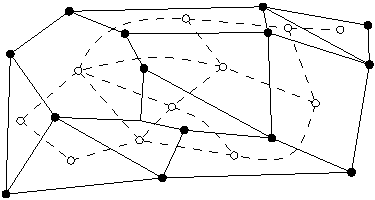
\includegraphics[width=0.45\textwidth]{figs/dual_graph}
  \caption{A graph $G$ (black lines), and its dual graph $G^\star$ (dashed lines).}
\label{fig:dual_graph}
\end{figure}
Observe that $G$ can also be seen as a cell complex in $\mathbb{R}^{2}$. 
The duality mapping is as follows (also shown in details in Figure~\ref{fig:dualdetailtab})
The dual graph $G^{\star}$ has a vertex for each face (polygon) in $G$, and the vertices in $G^{\star}$ are linked by an edge if and only if the two corresponding dual faces in $G$ are adjacent (in Figure~\ref{fig:dual_graph}, $G^{\star}$ is represented with dashed lines). 
Notice also that each polygon in $G^{\star}$ corresponds to a vertex in $G$, and that each edge of $G$ is actually dual to one edge (an arc in Figure~\ref{fig:dual_graph}) of $G^{\star}$ (for the sake of simplicity the dual edges to the edges on the boundary of $G$ are not drawn).

The VD and the DT are the best example of the duality between plane graphs.

\begin{figure}[h]
% \centering
% \setcapindent{1em}
\centering
\begin{minipage}[c]{0.4\textwidth}
  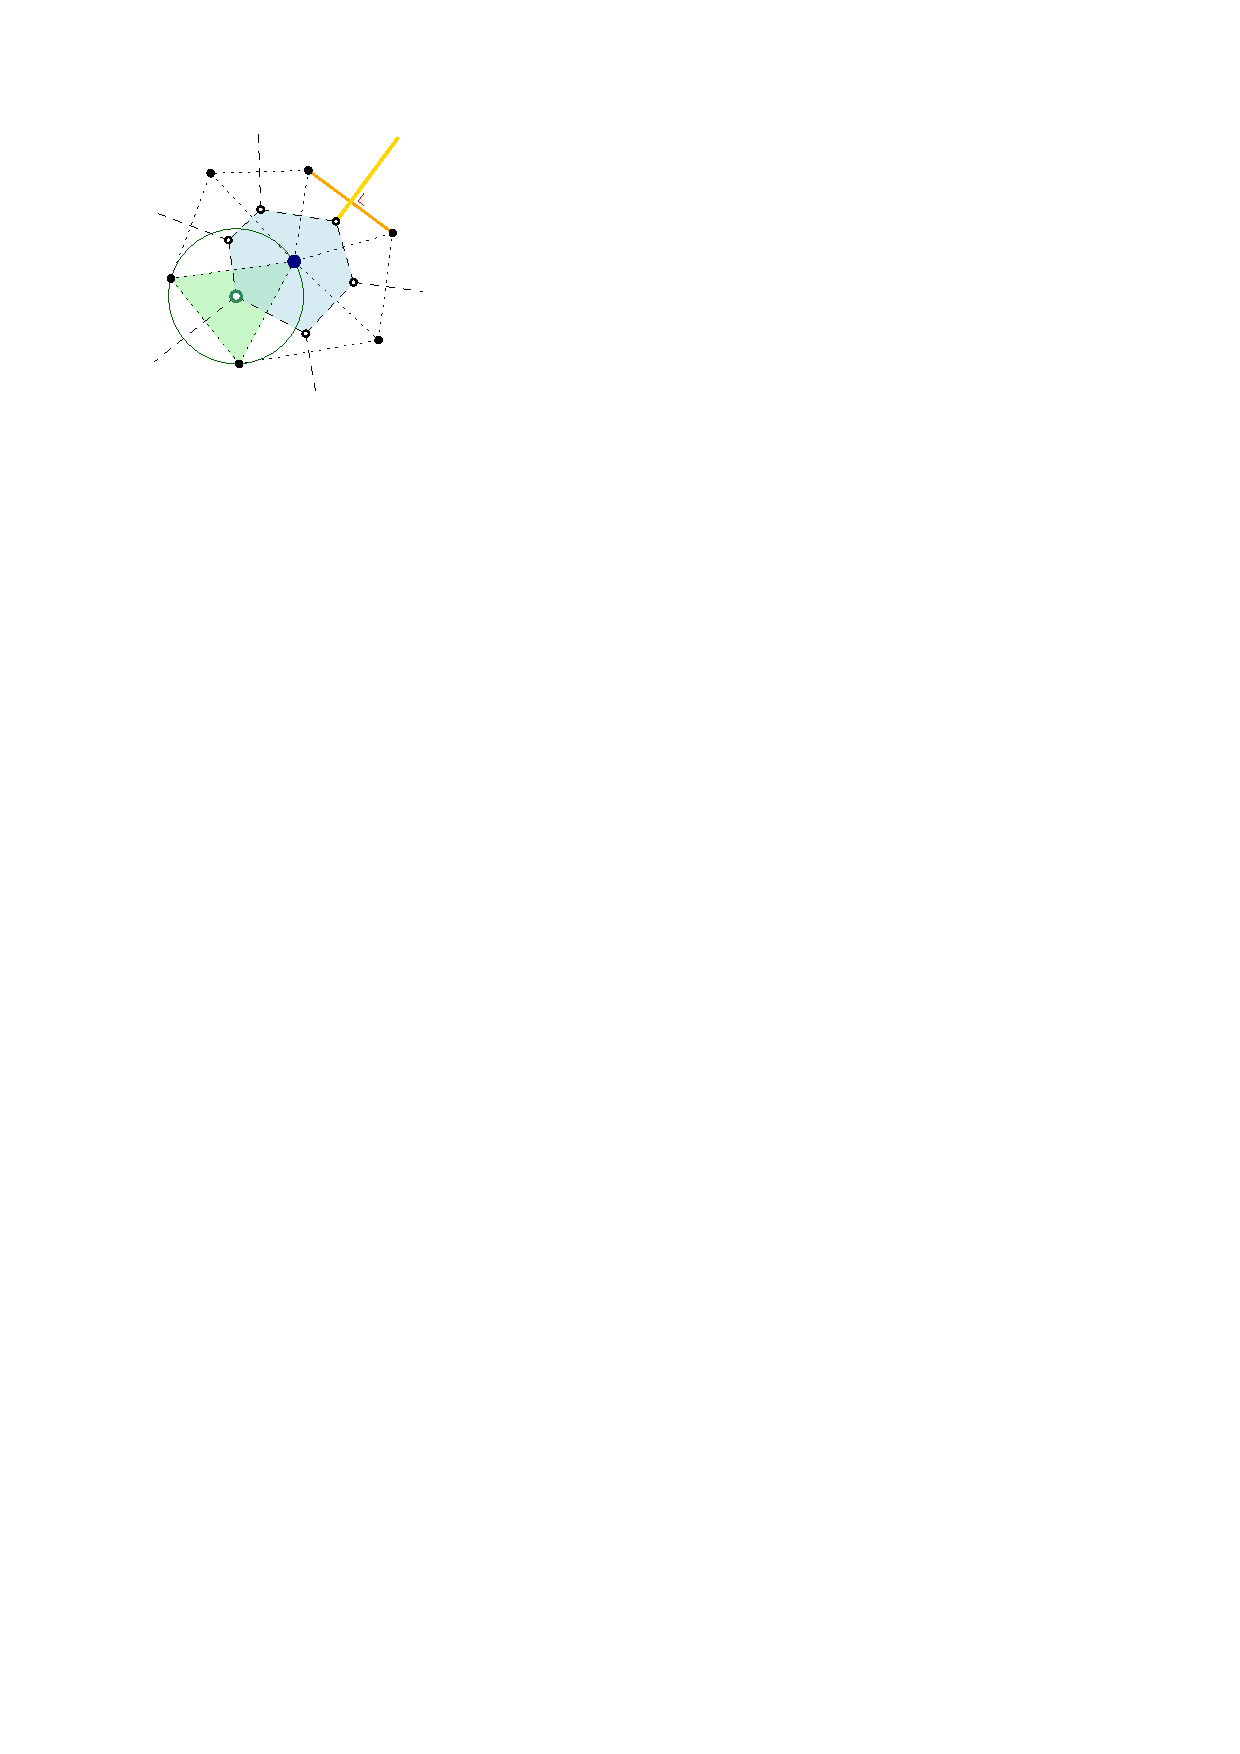
\includegraphics[width=\textwidth]{figs/dualdetail.pdf}
\end{minipage}
\begin{minipage}[c]{0.45\textwidth}
% \hspace{1.1em}
  \centering
  \begin{tabular}{lcl}
  \toprule
  DT & & VD \\
  \midrule
  $\mathbf{\color{YellowGreen}{face}}$ & $\leftrightarrow$ & $\mathbf{\color{ForestGreen}{vertex}}$\\
  $\mathbf{\color{Blue}{vertex}}$ & $\leftrightarrow$ & $\mathbf{\color{SkyBlue}{face}}$\\
  $\mathbf{\color{Orange}{edge}}$ & $\leftrightarrow$ & $\mathbf{\color{Dandelion}{edge}}$\\
  \bottomrule
  \end{tabular}
\end{minipage}
\caption{Duality between the DT (dotted) and the VD (dashed).}
\label{fig:dualdetailtab}
\end{figure}


%%%
%
\section{Incremental construction of the DT}

Since the VD and the DT are dual structures, the knowledge of one implies the knowledge of the other one. 
In other words, if one has only one structure, she can always extract the other one. 
Because it is easier, from an algorithmic and data structure point of view, to manage triangles over arbitrary polygons (they have a constant number of vertices and neighbours), constructing and manipulating a VD by working only on its dual structure is simpler and usually preferred. 
When the VD is needed, it is extracted from the DT\@. 
This has the additional advantage of speeding up algorithms because when the VD is used directly intermediate Voronoi vertices---that will not necessarily exist in the final diagram---need to be computed and stored.

%

While there exists different strategies to construct at DT, we focus here on the \emph{incremental} method (since it is easier to understand and implement).
An incremental algorithm is one where the structure is built incrementally; in our case this means that each point is inserted one at a time in a valid DT and the triangulation is updated, with respect to the Delaunay criterion (empty circumcircle), after each insertion. 
Observe that the insertion of a single point $p$ in a DT modifies only locally the DT, \ie\ only the triangles whose circumcircle contains $p$ need to be deleted and replaced by new ones respecting the Delaunay criterion (see Figure~\ref{fig:insertion_deletion}
\begin{figure}
  \centering
  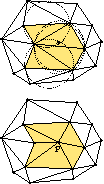
\includegraphics[width=0.6\textwidth]{figs/insertion_deletion}
  \caption{The DT before and after a point $p$ has been inserted. Notice that the DT is updated only locally (only the shaded part of the triangulation is affected).} 
\label{fig:insertion_deletion}
\end{figure}
for an example). 
In sharp contrast to this, other strategies to construct a DT (\eg\ divide-and-conquer and plane sweep algorithms, see Section~\ref{sec:notes}), build a DT in \emph{one} operation (this is a batch operation), and if another point needs to be inserted after this, the whole construction operation must be done again from scratch. 
That hinders their use for some applications where new data coming from a sensor would have to be added.


\begin{figure}
  \centering
  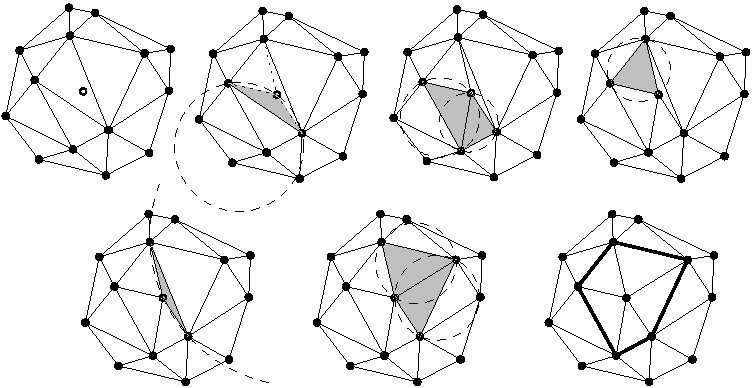
\includegraphics[width=1.0\textwidth]{figs/insertion_steps}
  \caption{Step-by-step insertion, with flips, of a single point in a DT in two dimensions.}
\label{fig:insertion_steps}
\end{figure}
\begin{algorithm}[tb] 
  \DontPrintSemicolon
  \KwIn{A DT($S$) $\mathcal{T}$ , and a new point $p$ to insert}
  \KwOut{$\mathcal{T}^{p} = \mathcal{T} \cup \{p\}$ // the DT with point $p$}
  find triangle $\tau$ containing $p$\;
  insert $p$ in $\tau$ by splitting it in to 3 new triangles\;
  push 3 new triangles on a stack\;
  \While{stack is non-empty}
  {
    $\tau = \{p,a,b\} \leftarrow$ pop from stack\;
    $\tau_{a} = \{a,b,c\} \leftarrow$ get adjacent triangle of $\tau$ having the edge $ab$\;
    \If{$c$ is inside circumcircle of $\tau$}
    {
      flip the triangles $\tau$ and $\tau_{a}$\;
      push 2 new triangles on stack\;
    }
  }
  \caption{Algorithm to insert one point in a DT}
\label{algo:insert1pt}
\end{algorithm} 

Figure~\ref{fig:insertion_steps} describes the algorithm, and Algorithm~\ref{algo:insert1pt} its pseudo-code. 
In a nutshell, for the insertion of a new point $p$ in a DT($S$), the triangle $\tau$ containing $p$ is identified and then split into three new triangles by joining $p$ to every vertex of $\tau$. 
Second, each new triangle is tested---according to the Delaunay criterion---against its opposite neighbour (with respect to $p$); if it is not a Delaunay triangle then the edge shared by the two triangles is \emph{flipped} (see below) and the two new triangles will also have to be tested later. 
This process stops when every triangle having $p$ as one of its vertices respects the Delaunay criterion.


%%%
\paragraph{Initialisation: the big triangle.}
\label{sec:big_tr}
Most of the incremental DT/VD algorithms assume that the set $S$ of points is entirely contained in a \emph{big triangle} ($\tau_{big}$) several times larger than the spatial extent of $S$; conv($S$) therefore becomes $\tau_{big}$. 
Figure~\ref{fig:big_tr} illustrates this.
\begin{figure}
  \centering
  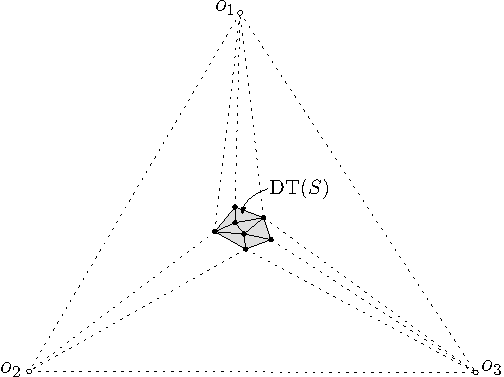
\includegraphics[width=0.45\textwidth]{figs/big_tr}
  \caption[The big triangle containing all the dataset.]{The set $S$ of points is contained by a \emph{big triangle} formed by the vertices $o_1$, $o_2$ and $o_3$. Many triangles outside conv($S$) are created.} 
\label{fig:big_tr}
\end{figure}
The construction of DT($S$) is for example always initialised by first constructing $\tau_{big}$, and then the points in $S$ are inserted one by one. 

%

Doing this has many advantages. 
First, when a single point $p$ needs to be inserted in DT($S$), this guarantees that $p$ is always inside an existing triangle; we thus do not have to deal explicitly with vertices added outside the convex hull. 
Second, we do not have to deal with the (nasty) case of deleting a vertex that bounds conv($S$). 
Third, since an edge is always guaranteed to be shared by two triangles, point location algorithms never ``fall off'' the convex hull. 
Fourth, identifying the vertices that bounds conv($S$) is easy: they have one incident triangle that has one or more of the big triangle vertices.
Fifth, the Voronoi cells of the points that bounds conv($S$) will be bounded, since the only unbounded cells will be the ones of the four points of $\tau_{big}$. 
This can help for some of the spatial analysis operations, for instance interpolation based on the VD (see Chapter~\ref{sec:interpol}).

%

The main disadvantage is that more triangles than needed are constructed. 
For example in Figure~\ref{fig:big_tr} only the shaded triangles would be part of DT($S$). 
The extra triangles can nevertheless be easily marked as they are the only ones containing at least one of the three points forming $\tau_{big}$. 

\begin{practice-box}
Several implementations/APIs of the DT use a big triangle (or variation of it with a ``point at the infinity'',  CGAL (\url{https://www.cgal.org/}) being one example), and these often label vertices and/or triangles as ``infinite''.
It is therefore essential to understand the mecanism, even if one is not constructing the DT herself.
\end{practice-box}


%%%
\paragraph{Walk/Point location.} To find the triangle containing the newly inserted point $p$, we can use the point-in-polygon test for every triangle (the standard GIS operation), but that would be too slow. 
A better alternative is to use the adjacency relationships between the triangles, and use a series of \Orient\ tests, as described below, to navigate from one triangle to the other. 
The idea, called ``walking'', is shown in Figure~\ref{fig:walk} and details are given in the Algorithm~\ref{algo:walk}.
\begin{figure}
  \centering
  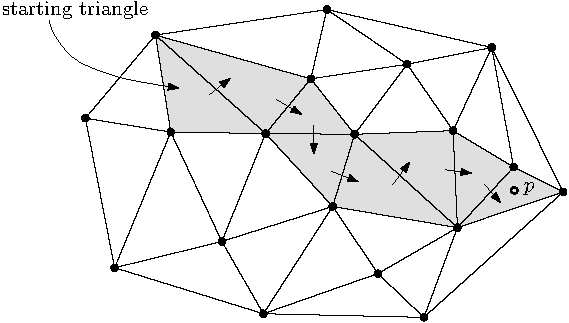
\includegraphics[width=0.5\textwidth]{figs/walk}
  \caption{The Walk algorithm for a DT in two dimensions. The query point is $p$.}
\label{fig:walk}
\end{figure}
\begin{algorithm}[t]
  \DontPrintSemicolon
  \KwIn{A DT($S$) $\mathcal{T}$, a starting triangle $\tau$, and a query point $p$}
  \KwOut{$\tau_r$: the triangle in $\mathcal{T}$ containing $p$}
  \BlankLine  
  \While{$\tau_r$ not found}
  {
    \For{$i \leftarrow 0$ \KwTo 2}
    {
      $\sigma_i \leftarrow$ get edge opposite vertex $i$ in $\tau$\;
      \If{\Orient($\tau_i, p$) $< 0$\nllabel{l:walk}} 
      {
        $\tau \leftarrow$ get neighbouring triangle of $\tau$ incident to $\sigma_i$\;
        break\;
      }
    }  
    \If{$i=2$}
    {
      \tcp{all the edges of $\tau$ have been tested}
      Return ($\tau_r$ = $\tau$)\;
    }
  }
  \caption{W\textsc{alk}($\mathcal{T}$, $\tau$, $p$)}
\label{algo:walk}
\end{algorithm}
The idea is as follows: in a DT($S$), starting from a triangle $\tau$ (it can be any), we move to one of the adjacent triangle of $\tau$ ($\tau$ has three neighbours, we choose one neighbour $\tau_i$ such that the query point $p$ and $\tau$ are on each side of the edge shared by $\tau$ and $\tau_i$) until there is no such neighbour, then the simplex containing $p$ is $\tau$.
Notice that this algorithm is not affected by degenerate cases, and that if an \textrm{O}\textsc{rientation} test returns 0 (collinearity), then it is simply considered a positive result. 
This will ensure that if the query point $p$ is located exactly at the same position as one point in $S$, then one triangle incident to $p$ will be returned.


%%%
\paragraph{Flips.}The \emph{flip} operation we use to modify the triangulation is a simple local topological operation that modifies the configuration of two adjacent triangles. 
Consider the set $S = \{a, b, c, d\}$ of points in the plane forming a quadrilateral, as shown in Figure~\ref{p:flip22}. 
\begin{figure}
  \centering
  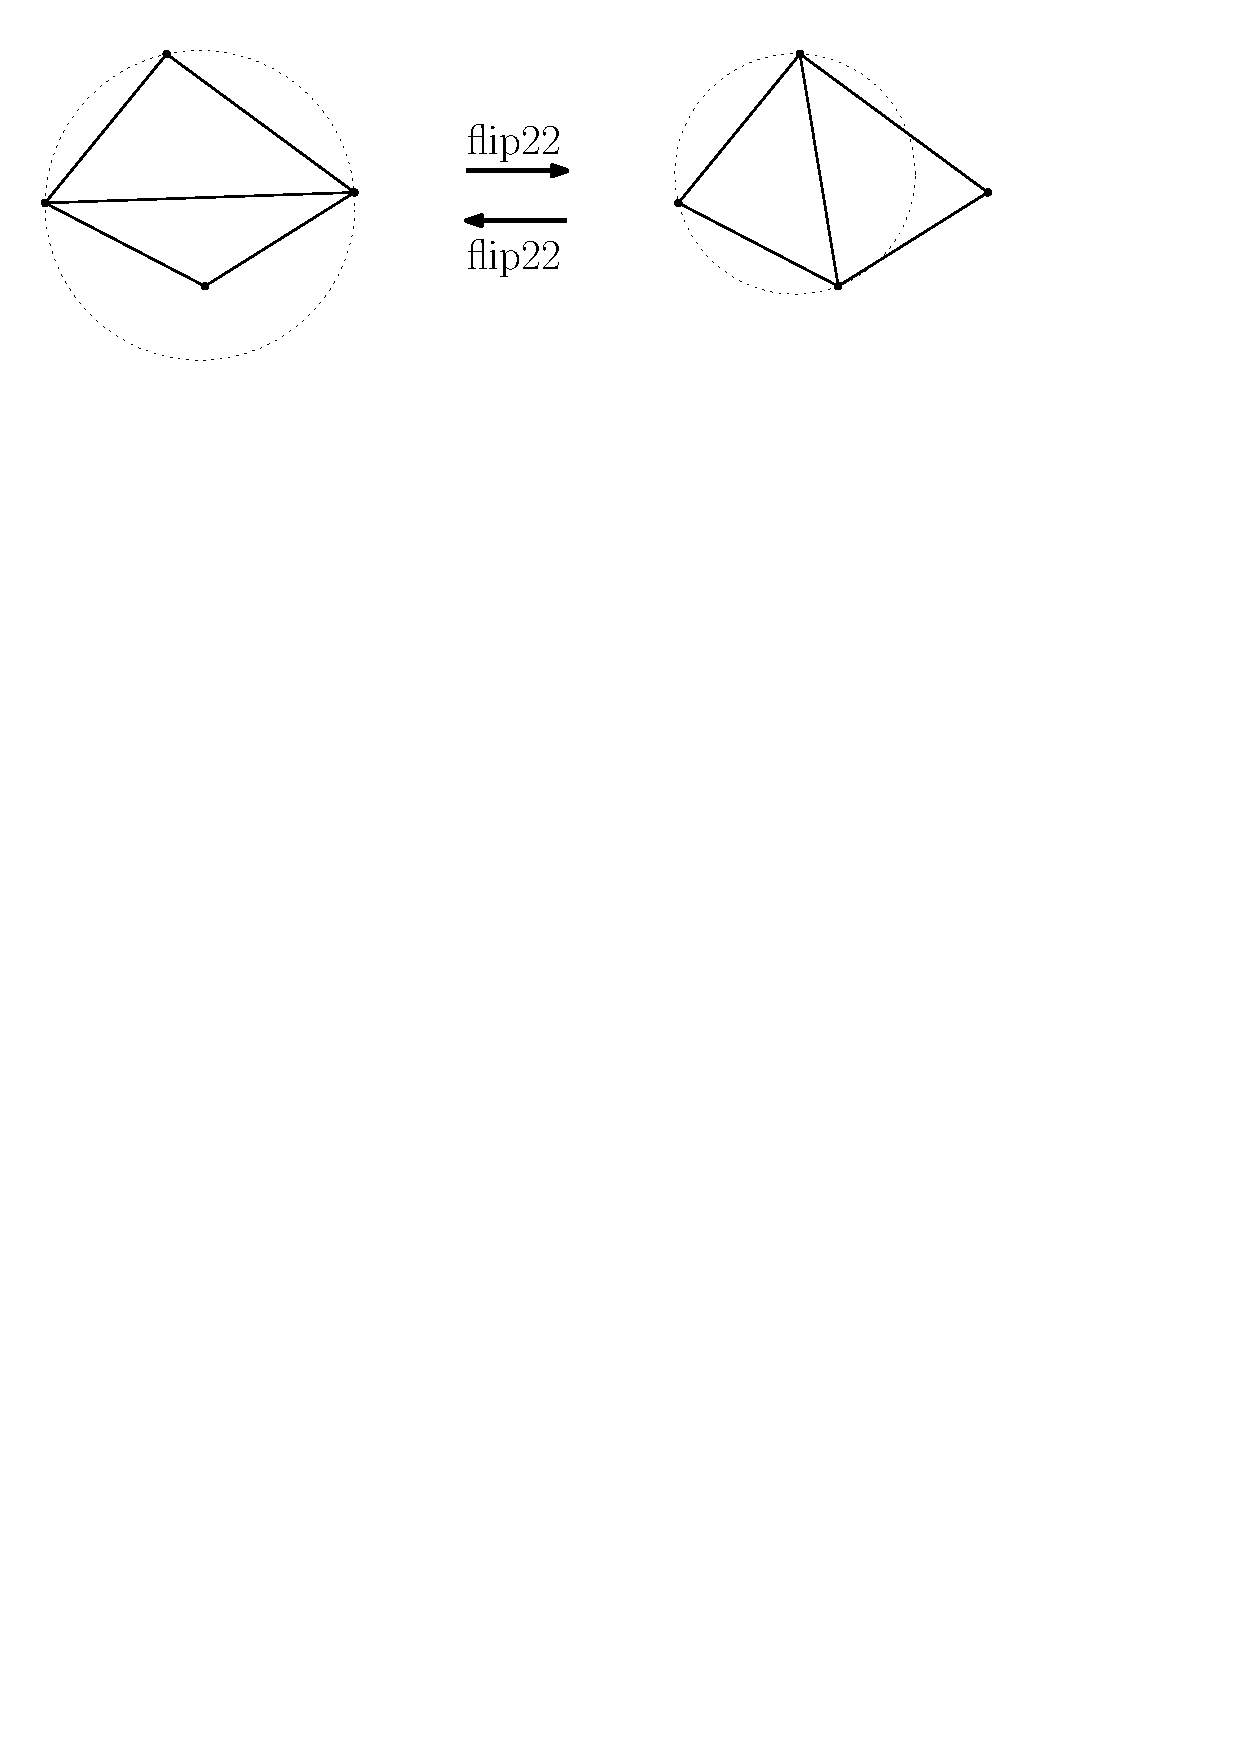
\includegraphics[width=0.5\textwidth]{figs/flip22}
  \caption{A flip22}
\label{p:flip22}
\end{figure}
There exist exactly two ways to triangulate $S$: the first one contains the triangles $abc$ and $bcd$; and the second one contains the triangles $abd$ and $acd$. 
Only the first triangulation of $S$ is Delaunay because $d$ is outside the circumcircle of $abc$. 
A \emph{flip} is the operation that transforms the first triangulation into the second, or vice-versa.


%%%
\paragraph{Controlling the flips.}
To control which triangles have to be checked and potentially flipped, we use a stack\footnote{A data structure: \url{https://en.wikipedia.org/wiki/Stack_(abstract_data_type)}}. 
When the stack is empty, then there are no more triangles to be tested, and we are guaranteed that all the triangles in the triangulation have an empty circumcircle.


%%%
\paragraph{Predicates.}
Constructing a DT and manipulating it essentially require two basic geometric tests (called \emph{predicates}): \Orient\ determines if a point $p$ is left, right or lies on the line segment defined by two points $a$ and $b$; and \Insphere\ determines if a point $p$ is inside, outside or lies on a circle defined by three points $a$, $b$ and $c$. 
Both tests can be reduced to the computation of the determinant of a matrix:
\begin{equation}
  \textrm{O}\textsc{rientation}(a, b, p) = 
  \left| 
  \begin{array}{cccc}
    a_{x} & a_{y} & 1 \\
    b_{x} & b_{y} & 1 \\
    p_{x} & p_{y} & 1 
  \end{array} 
  \right| 
\end{equation}
\begin{equation}
  \textrm{I}\textsc{n}\textrm{C}\textsc{ircle}(a, b, c, p) = 
  \left| 
  \begin{array}{ccccc}
    a_{x} & a_{y} & a^{2}_{x} + a^{2}_{y} & 1 \\
    b_{x} & b_{y} & b^{2}_{x} + b^{2}_{y} & 1 \\
    c_{x} & c_{y} & c^{2}_{x} + c^{2}_{y} & 1 \\
    p_{x} & p_{y} & p^{2}_{x} + p^{2}_{y} & 1 
  \end{array} 
  \right|
\label{eq:insphere}
\end{equation}


%%%%%%%%%%%%%%%%%%%%%%%%%%%%
%%%%%%%%%%%%%%%%%%%%%%%%%%%%
\section{Data structures for storing a DT}

A triangulation is simply a subdivision of the plane into polygons, and thus any data structure used in GIS can be used to store a triangulation.

\begin{description}
  \item[Simple Features:] while many use this (PostGIS and any triangulation you see in Shapefiles), this is not very smart: (1) the topological relationships between the triangles are not stored; (2) the vertices are repeated for each triangle (and we know that for a Poisson distribution of points in the plane a given point has exactly 6 incident triangles).
  \item[edge-based structures:] all the edge-based topological data structure discussed in GEO1002 (DCEL, half-edge, winged-edge, etc) can be used. These usually lead to large storage space.
\end{description}

Observe that in practice, if only the DT is wanted (and not the constrained one, see below), practitioners will often simply store the sample points and reconstruct on-the-fly the DT, since it is unique (if we omit points not in general position that is).

However, because it is simpler to manage triangles over arbitrary polygons (they always have exactly 3 vertices and 3 neighbours), data structures specific for triangulations have been developed and are usually used.

The simplest data structure, as shown in Figure~\ref{fig:tr_ds}, 
\begin{figure}
  \centering
  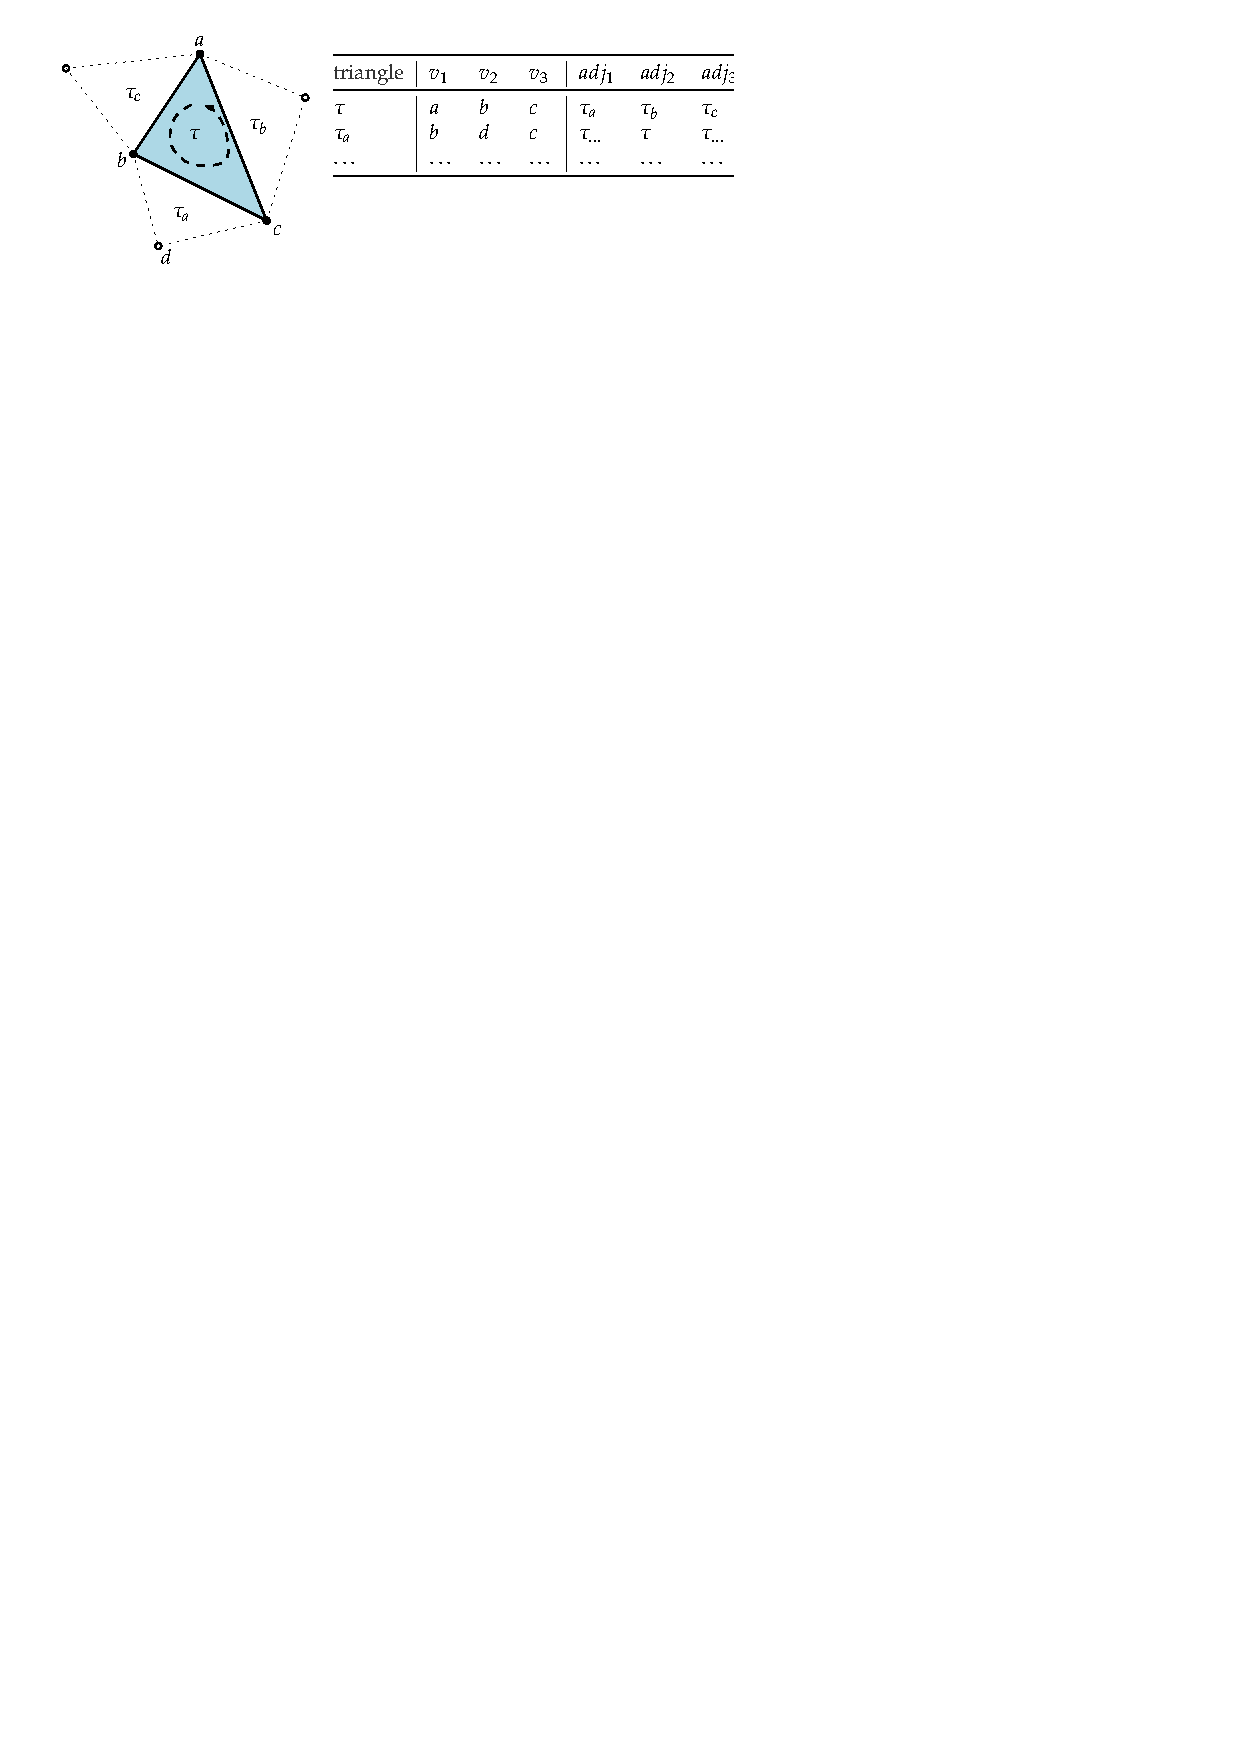
\includegraphics[width=0.95\linewidth]{figs/tr_ds}
  \caption{The triangle-based data structure to store efficiently a triangulation (and the adjacency relationships between the triangles).}
\label{fig:tr_ds}
\end{figure}
considers the triangle as being its atom and stores each triangle with 3 pointers to its vertices and 3 pointers to its adjacent triangles. 




%%%%%%%%%%%%%%%%%%%%%%%%%%%%
\section{Constrained and Conforming Delaunay Triangulations}

Given as input a set $S$ of points and straight-line segments in the plane, different triangulations of $S$ (so that the segments are respected) can be constructed. 
We are mostly interested in the \emph{constrained Delaunay triangulation} (ConsDT) and the \emph{conforming Delaunay triangulation} (ConfDT).
\begin{figure}
  \centering
  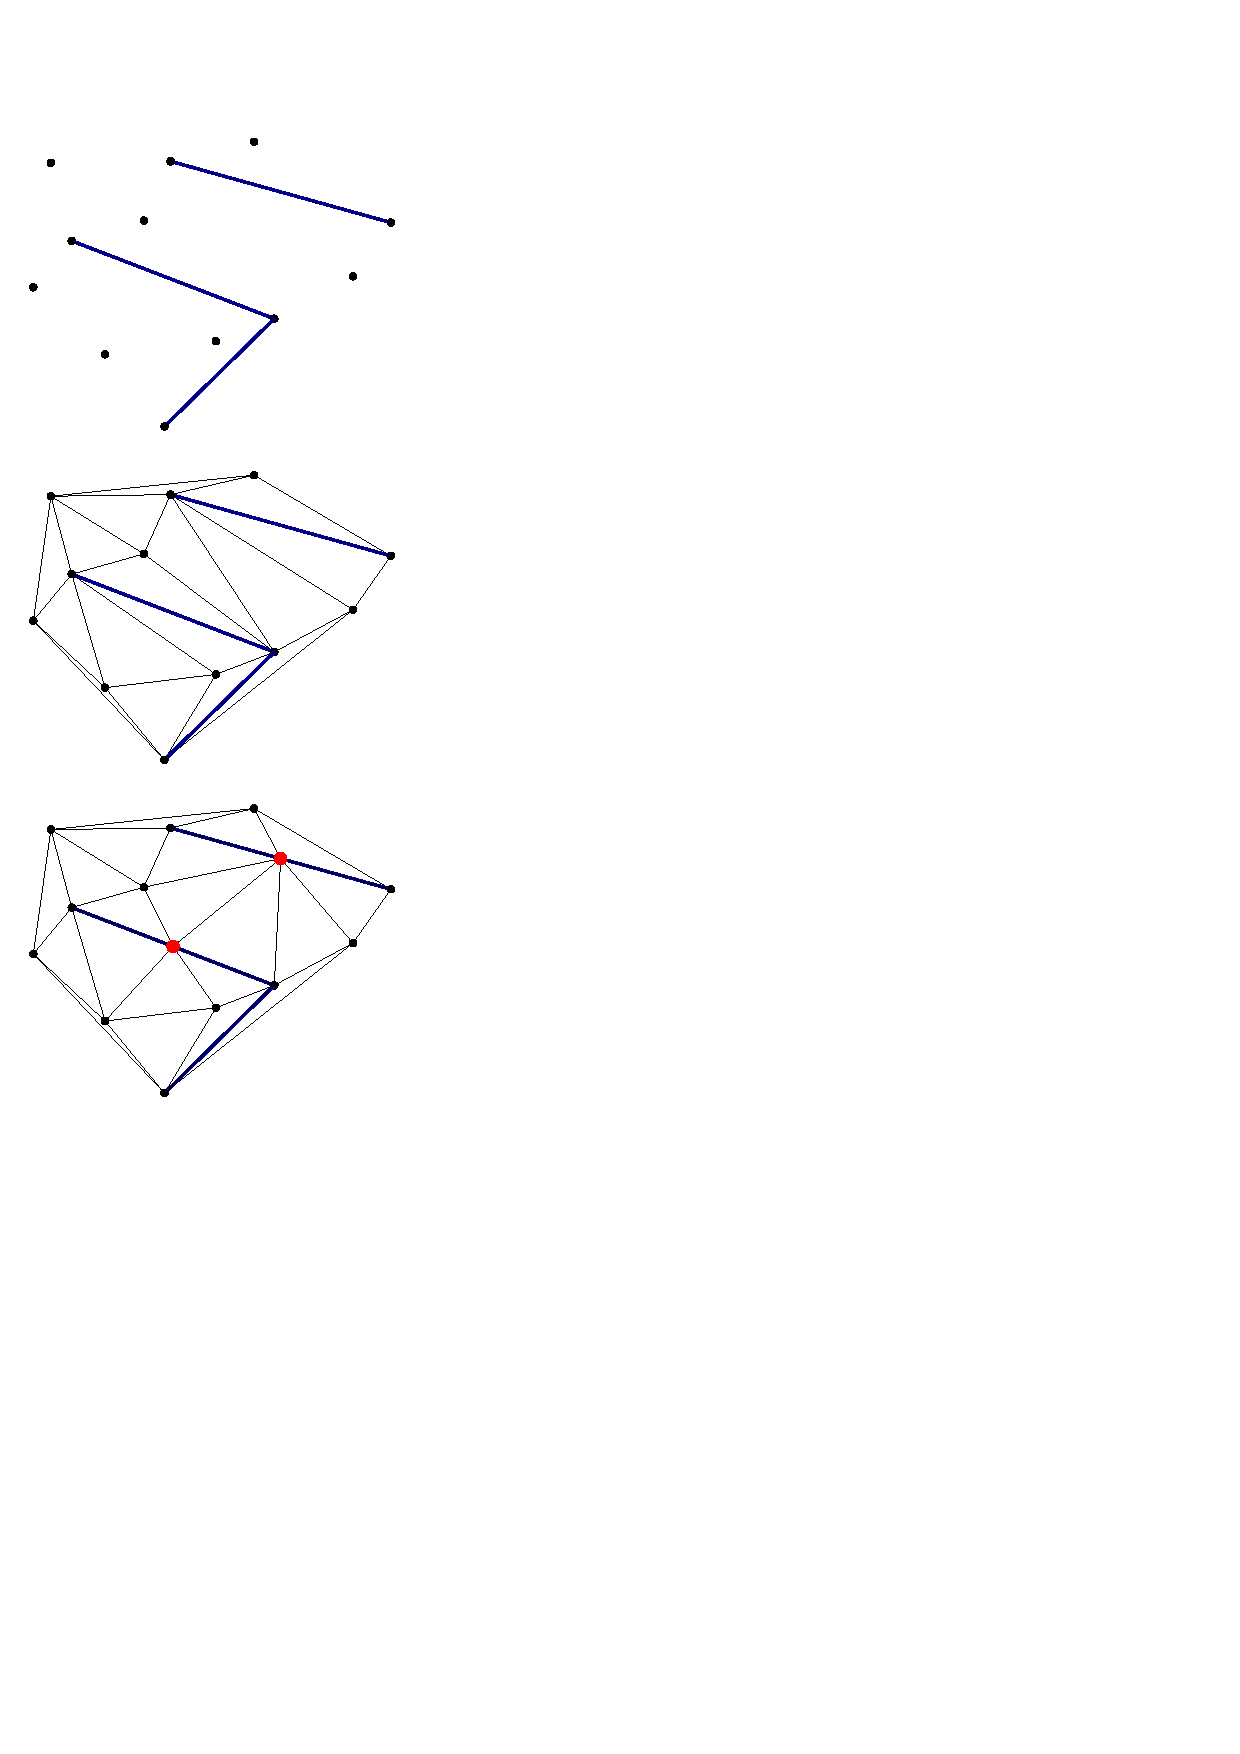
\includegraphics[width=\linewidth]{figs/cdt_example}
  \caption{\textbf{(a)} A a set $S$ of points and straight-line segments. \textbf{(b)} Constrained DT of $S$. \textbf{(c)} Conforming DT of $S$; the Steiner points added are in red.}
\label{fig:cdt_example}
\end{figure}

%%%
%
\paragraph*{Constrained DT (ConsDT).}
Given a set $S$ of points and straight-line segments in $\mathbb{R}^2$, the ConsDT permits us to decompose the convex hull of $S$ into non-overlapping triangles, and every segment of $S$ appears as an edge in ConsDT($S$). 
ConsDT is similar to the Delaunay triangulation, but the triangles in ConsDT are not necessarily Delaunay (\ie\ their circumcircle might contain other points from $S$). 
The empty circumcircle for a ConsDT is less strict: a triangle is Delaunay if its circumcircle contains no other points in $S$ that are \emph{visible} from the triangle.
The constrained segments in $S$ act a visibility blockers. 
Figure~\ref{fig:cdt_buildings} shows one example.
\begin{figure}
  \centering
  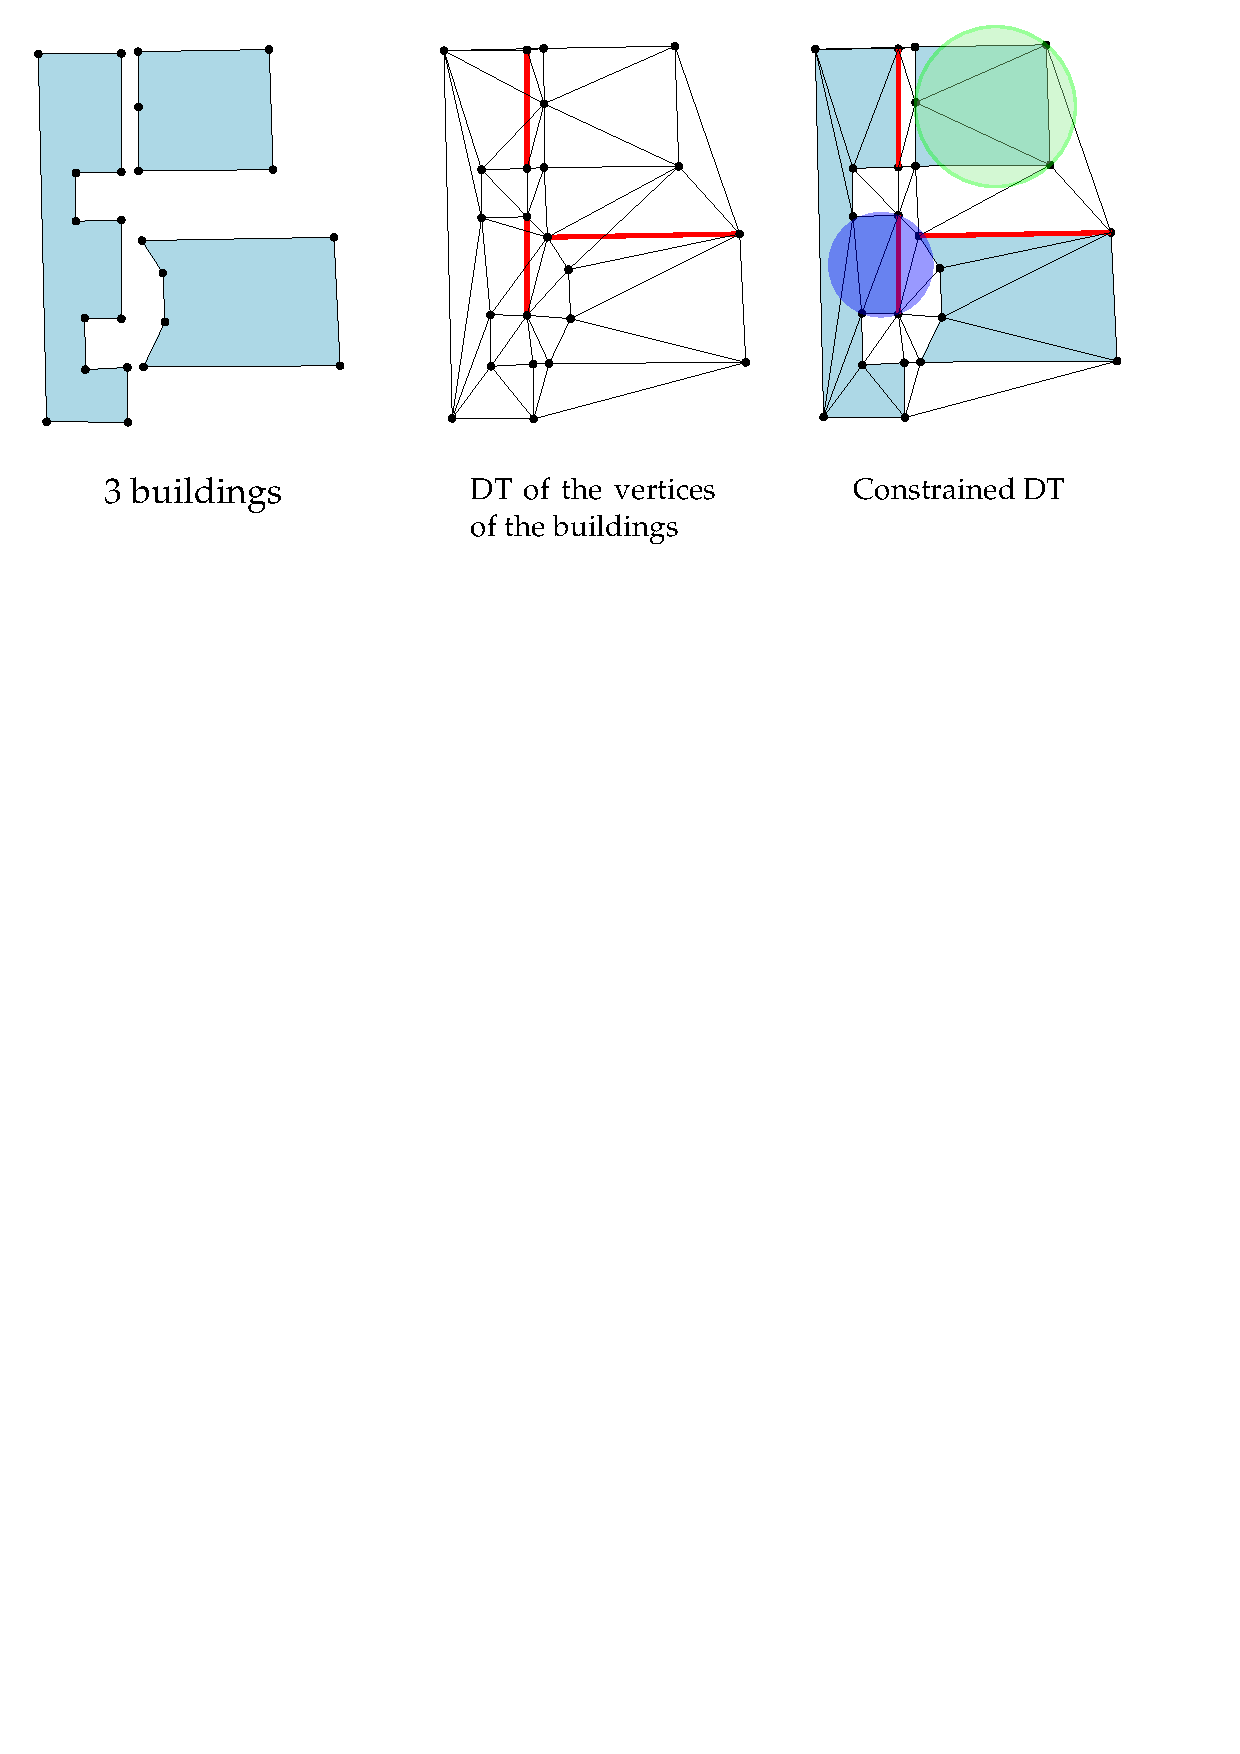
\includegraphics[width=0.95\textwidth]{figs/cdtbuildings}
  \caption{The ConsDT of a set of segments. On the right, the triangle whose circumcircle is green is a Delaunay (no other points in its interior) and so is the triangle whose circumcircle is in blue (there is one point in its interior, but it cannot be seen because of the constrained segment).}
\label{fig:cdt_buildings}
\end{figure}

%

Without going into details about one potential algorithm, one way to construct a ConsDT($S$) is (see Figure~\ref{fig:cdt_steps}:
\begin{figure}
  \centering
  \includegraphics[width=0.95\linewidth]{figs/cdt_steps}
  \caption{Steps to construct a ConsDT.}
\label{fig:cdt_steps}
\end{figure}
\begin{enumerate}
  \item construct DT($S^p$), where $S^p$ is the set containing all the points in $S$ and the end points of the line segments (Figure~\ref{fig:cdt_steps}b)
  \item insert each line segment, each insertion will remove edges from DT($S^p$). In Figure~\ref{fig:cdt_steps}c 3 edges are removed.
  \item this creates 2 polygons that need to be retriangulated, in Figure~\ref{fig:cdt_steps}d there is a blue and a green one.
  \item retriangulate each separately, the Delaunay criterion needs to be verified only for the vertices incident to the triangles incident to the hole/polygon.
\end{enumerate}

%

Observe that the ConsDT can be used to triangulate polygons with holes(see Figure~\ref{fig:cdt_dog}, it suffices to remove the triangle outside the exterior boundary, but inside the convex hull.
\begin{figure}
  \centering
  \includegraphics[width=0.6\linewidth]{figs/cdt_dog}
  \caption{\textbf{Left}: One polygon with 4 holes (interior rings). \textbf{Right}: its ConsDT.}
\label{fig:cdt_dog}
\end{figure}


%%%
%
\paragraph*{Conforming DT (ConfDT).}
A ConfDT adds new points to the input $S$ (called \emph{Steiner} points) to ensure that the input segments are present in the triangulation. 
As Figures~\ref{fig:ccdt} and ~\ref{fig:cdt_example}c show, the input straight-line segments will be split into several collinear segments. 
The Steiner points have to be carefully chosen (where to put them is beyond the scope of this course).
\begin{figure}
  \centering
  \begin{subfigure}[b]{0.3\linewidth}
    \includegraphics[width=\textwidth]{figs/cdt_input.pdf}
    \caption{}
  \end{subfigure}%
  \qquad
  \begin{subfigure}[b]{0.3\linewidth}
    \includegraphics[width=\textwidth]{figs/cdt.pdf}
    \caption{}
  \end{subfigure}%
  \qquad
  \begin{subfigure}[b]{0.3\linewidth}
    \includegraphics[width=\textwidth]{figs/cdt_conf.pdf}
    \caption{}
  \end{subfigure}%
  \caption{\textbf{(a)} Input polygon (or set of segments). \textbf{(b)} ConsDT of the input. \textbf{(c)} ConfDT of the input.}
\label{fig:ccdt}
\end{figure}
Observe that each triangle in a ConfDT respect the Delaunay criterion, but that more triangles are present. 
If 2 segments are nearly parallel, many points could be necessary (for $m$ segments, up to $m^2$ could be necessary).

%%%%%%%%%%%%%%%%%%%%%%%%%%%%
%%%%%%%%%%%%%%%%%%%%%%%%%%%%
\section{Triangulation of a polygon}

We describe here algorithms to decompose a polygon into non-overlapping triangles (that are not necessarily Delaunay).
While this is not directly related to the modelling of terrains (where we do not have polygons, usually), the topic is relevant in GIS and, as seen below, constrained are often used in terrains.

It is known that any simple polygon (even with holes) can be triangulated without adding new vertices.

%%%
%
\subsection{The trivial case of a convex polygon}

If the polygon to triangulate is convex, then triangulating it is trivial with a \emph{fan-shaped triangulation}.
As shown in Figure~\ref{fig:fanshaped},
\begin{figure}
  \centering
  \begin{subfigure}[b]{0.35\linewidth}
    \centering
    \includegraphics[page=1,width=\textwidth]{figs/fanshaped}
    \caption{}
  \end{subfigure}%
  \qquad
  \begin{subfigure}[b]{0.35\linewidth}
    \centering
    \includegraphics[page=2,width=\textwidth]{figs/fanshaped}
    \caption{}
  \end{subfigure}
\caption{Fan-shaped triangulation of a convex polygon.}
\label{fig:fanshaped}
\end{figure}
the algorithm is simple: starting from an arbitrary vertex $v$ of the polygon $P$, and add edges joining $v$ to all other vertices of $P$, except the previous and next vertices in the ordered boundary of $P$.
A polygon $P$ with $n$ vertices will be triangulated into ($n-2$) triangles.



%%%
%
\subsection{Greedy algorithm for polygons with holes}

A greedy algorithm makes at each step the \emph{locally} optimal choice, and does not look at what has been done before (it never goes back). 
It is very simple to understand and implement, but can yield a very slow implementation.

A greedy algorithm to triangulation a simple polygon $P$ is described in Algorithm~\ref{algo:greedy}.
\begin{algorithm}[tb] 
  \KwIn{Simple polygon $P$ with $n$ vertices}
  \KwOut{Triangulation $\mathcal{T}$ of $P$}
  from the set $D$ of $m=\frac{n(n-3)}{2}$ diagonals of $P$\;
  sort $D$ into ascending order of length $d_1, \ldots, d_m$\;
  triangulation $\mathcal{T} \leftarrow P$\;
  \For{$i \leftarrow 1$ to $m$}
  {
    \If{$d_i$ does not intersect segments in $\mathcal{T}$ AND $d_i$ is an internal diagonal of $P$}
    {
      $\mathcal{T} \leftarrow \mathcal{T} \cup d_i$\;
    }
  }
  \caption{A greedy algorithm to triangulate a simple polygon.}
\label{algo:greedy}
\end{algorithm}
The algorithm basically finds all the potential diagonals for $P$ (all the pairs of vertices), sort them based on their length (ascending length), and at each step of the algorithm the shortest diagonal is inserted if it does not intersect with other already inserted diagonals, and if it is inside $P$. 
Diagonals that have been inserted are never removed. 
When all the possible diagonals have been inserted, each triangle must be constructed by finding 3 segments (boundary of $P$ and diagonals). 
The algorithm is valid for polygon with holes, since all the possible combination of diagonals could be tried.


%%%
%
\subsection{Ear clipping for polygons without holes}

An alternative---and faster---method is by using the ``ear clipping'' algorithm. 
As shown in Figure~\ref{fig:earclipping},
\begin{figure}
  \centering
  \includegraphics[width=\textwidth]{figs/earclipping}
  \caption{Ear clipping algorithm and the various steps to obtain the triangulation; that last steps are missing.}
\label{fig:earclipping}
\end{figure}
an ear is defined as 3 consecutive points of a polygon forming a triangle; $abc$ is a valid ear of the input polygon $P$, but $cde$ is not (because the triangle is outside the polygon) and neither is $fgh$ (because $d$ is inside the ear).. 
The idea of the ear clipping algorithm is to identify a valid ear, remove it from the polygon and repeat this process (with the modified polygon) until only one triangle is left. 
The implementation is simple: simply keep a list of ordered vertices and each removal of an ear simply removes one vertex (in Figure~\ref{fig:earclipping} at the first step the vertex $b$ is removed).

Observe that this algorithm does not work with polygon having holes.

Finding a valid ear of a simple polygon $P$ is relatively easy: if the points are ordered CCW on the boundary of $P$, then 3 consecutive points must have a positive \Orient; and to verify that the ear is completely inside $P$ the other points of $P$ must be outside that triangle (for instance in Figure~\ref{fig:earclipping} the point $d$ would be inside the triangle $fgh$).


%%%
%
\section{Notes and comments}
\label{sec:notes}

For the construction of the DT, the incremental algorithm we use was first described by \citet{Lawson72-1}.
\citet{Guibas85} describe a divide-and-conquer algorithm, and \citet{Fortune87} a sweep-line one.

The local optimality of a DT, which implies globally optimality in the case of the DT, was proven by \citet{Delaunay34} himself.
The \emph{max-min angle optimality} of the DT was firstly observed by \citet{Sibson78}.
This paraboloic lifting was first observed by \citet{Brown79} (who used a spherical transformation), further described by \citet{Seidel82,Edelsbrunner86}. 

Instead of using a \emph{big triangle}, several will use an ``infinite point'' or a ``far-away point'', which is conceptually the same but numerically more stable (since the size of the big triangle does not need to be defined).
\citet{Liu05-1} explains the details.

The walking in the triangulation to location the triangle containing a newly inserted point is not \emph{per se} the fastest solution, \citet{Mucke99} and \citet{Devillers02} discuss alternatives.
They both note that optimal algorithms do not necessarily mean better results in practice because of the amount of preprocessing involved, the extra storage needed, and also because the optimal algorithms do not always consider the dynamic case, where points in the DT could be deleted. 

The fact that the DT is computed only in 2D (without taking into account the elevation of the vertices) has been criticised by several as sub-optimal for the modelling of terrain.
To remedy to this, \citet{Dyn90} develop a \emph{data-dependent algorithm}, and \citet{Gudmundsson02} propose using \emph{higher-order} Delaunay triangulations (a modification where the empty circumcircle is also based on the neighbours of the neighbours).
Nevertheless, there are still results stating that the Delaunay triangulation is still the one that minimises the roughness of a surface~\citep{Wang01,Rippa90}

% TODO : complete this: uniqueness of the DT
% If the input points of the DT are not in general position, it is still possible to obtain a unique DT\@.
% This however means that 

The Algorithm~\ref{algo:greedy}, is taken from \citet[p. 202]{Worboys04}.

\citet{Shewchuk97} shows that while the triangle-based data structure requires twice as much code as with the quad-edge (to store and construct a ConsDT), the result is that the code runs twice as fast and the memory requirement as about 2X less.
CGAL (\url{https://www.cgal.org/}), among many others, uses the triangle-based data structure.


%!TEX root = ../terrainbook.tex
% chktex-file 46

\setchapterpreamble[u]{\margintoc}
\chapter{Spatial interpolation: deterministic methods}%
\label{chap:interpol}



\graphicspath{{interpol/}}



% \chaptertoc

Given a set $S$ of points $p_i$ in $\mathbb{R}^2$ (also called samples or data points in the following) to which an attribute $a_i$ is attached, spatial interpolation is the procedure used to estimate the value of the attribute at an unsampled location $x$. 
Its goal is to find a function $f(x,y)$ that fits (passes through, or close to, all the points in $S$) as well as possible. 
There is an infinity of such functions, some are global and some are piecewise, the aim is to find one that is best suited for the kind of datasets used as input.
Interpolation is based on \emph{spatial autocorrelation},% 
\index{spatial autocorrelation}
that is the attribute of two points close together in space is more likely to be similar than that of two points far from each other.

%

\begin{marginfigure}
  \centering
  \includegraphics{figs/extrapolation}
  \caption{Spatial interpolation and extrapolation.}%
\labfig{fig:extrapolation}
\end{marginfigure}
It should be noticed that the natural spatial extent of a set of sample is its \emph{convex hull}, and that an estimation outside this convex hull is \emph{extrapolation} (\reffig{fig:extrapolation}).\index{extrapolation}
Extrapolating implies that more uncertainty is attached to the estimated value.

%

Spatial interpolation methods are crucial in the visualisation process (\eg\ generation of contours lines), for the conversion of data from one format to another (\eg\ from scattered points to raster), to have a better understanding of a dataset, or simply to identify `bad' samples. 
The result of interpolation---usually a surface that represents the terrain---must be as accurate as possible because it often forms the basis for spatial analysis, for example runoff modelling or visibility analysis. 
Although interpolation helps in creating three-dimensional surfaces, in the case of terrains it is intrinsically a two-dimensional operation because only the ($x,y$) coordinates of each sample are used, and the elevation is the dependent attribute.
Notice that the attribute used need not be only elevation, for other GIS applications one could use the spatial interpolation methods below for for instance rainfall amounts, percentage of humidity in the soil, maximum temperature, etc. 
Spatial interpolation in 3D is also possible (but out of scope for this book), in that case there are 3 independent variables ($x,y,z$) and one dependent variable, for instance the temperature of the sea at different depth, or the concentration of a certain chemical in the ground.


%


%-------------------------------------------------
%%%
\section{What is a good interpolation method for terrains?}

The essential properties of an `ideal' interpolation method for bivariate\index{bivariate function} geoscientific datasets are as follows:
\begin{enumerate}
  \item \textbf{exact}: the interpolant must `honour' the data points, or `pass through' them.
  \item \textbf{continuous}: a single and unique value must be obtained at each location. This is called a $C^0$ interpolant\index{$C^n$ interpolants} in mathematics (see \reffig{fig:continuity}).
  \item \textbf{smooth}: it is desirable for some applications to have a function for which the first or second derivative is possible everywhere; such functions are respectively referred to as $C^1$ and $C^2$ interpolants.
  \item \textbf{local}: the interpolation function uses only some neighbouring samples to estimate the value at a given location. This ensures that a sample with a gross error will not propagate its error to the whole interpolant.
  \item \textbf{adaptability}: the function should give realistic results for anisotropic data distributions and/or for datasets where the data density varies greatly from one location to another.
  \item \textbf{computationally efficient}: it should be possible to implement the method and get an efficient result. Efficiency is of course subjective. For a student doing this course, efficiency might mean that the method generates a result in matter of minutes or an hour on a laptop, for the homework dataset. For a mapping agency, running a process for a day on a supercomputer for a whole country might be efficient. Observe that the complexity of the algorithm is measured not only on the number $n$ of points in the dataset, but how many neighbours $k$ are used to perform one location estimation.
  \item \textbf{automatic}: the method must require as little input as possible from the user, \ie\ it should not rely on user-defined parameters that require \emph{a priori} knowledge of the dataset.
\end{enumerate}
\begin{figure}
  \centering
  \includegraphics[width=\linewidth]{figs/continuity}
  \caption{$C^0$ interpolant is a function that is continuous but the first derivative is not possible at certain locations; $C^1$ interpolant has its first derivative possible everywhere; $C^2$ interpolant has its second derivative possible everywhere (this one is more difficult to draw).}%
\labfig{fig:continuity}
\end{figure}



%-------------------------------------------
%-
\section{Fitting polynomials}


%%%
%
\subsection{One global function}

We know that if we have $n$ points in $S$ (in $\mathbb{R}^3$ since the samples are lifted to their elevation), there exists at least one polynomial of degree at most $n-1$.

This interpolant will be exact, continuous and smooth (at least $C^2$).
However, it will not be local (which is problematic for terrains), and finding the polynomial of a high degree for large datasets might be impossible (or take a lot of time).

The biggest concern polynomials is probably that while the interpolant is exact (the surface passes through the sample points), higher-degree polynomials can oscillate between the samples and `overshoot', \ie\ be (far) outside the minimum or maximum $z$ values of the the set $S$.
This is known as the Runge's phenomenon in numerical analysis,%
\index{Runge's phenomenon }\marginnote{Runge's phenomenon}
and is shown in \reffig{fig:polynomial}.
\begin{figure*}
  \centering
  \includegraphics[width=\linewidth]{figs/polynomial}
  \caption{A few of the interpolation methods shown for a 1D dataset. \textbf{(a)} Input sample points. \textbf{(b)} Polynomial fitting, and the Runge's effect shown. \textbf{(c)} Natural neighbour. \textbf{(d)} Linear interpolation in TIN.}%
\labfig{fig:polynomial}
\end{figure*}



%%%
%
\subsection{Splines: piecewise polynomials}%
\index{splines}

Splines are piecewise polynomials, each piece is connected to its neighbouring piece in a \emph{smooth} manner: along the edges and at the data points the function is usually still $C^1$ or $C^2$ (in other words, where 2 or more polynomials connect, they have the same values for their tangents).

In practice, for terrain modelling, splines are preferred over one polynomial function because of the reasons mentioned above (mostly Runge's effect) and because computing the polynomial for large datasets is very inefficient.
The polynomials used in each piece of the subdivision is usually of low degree ($\leq 5$)

%

There are several types of splines (and variation of them, such as Bézier), and most of them are not suited for terrains.
The most used spline in practice seems to be the \emph{regularised spline with tension} (RST)\marginnote{regularised spline with tension is available in the open-source GIS GRASS}, where the dataset is decomposed into square pieces of a certain size.
The Runge's effect (also called \emph{overshoots}) are eliminated (since the degree is low), and the tension parameter can be tuned to obtain an interpolant that is smooth.




%-------------------------------------------
%-
\section{Weighted-average methods}

The five interpolation methods discussed in this section are \emph{weighted-average methods}.
These are methods that use a subset of the sample points, to which a weight (importance) are assigned, to estimate the value of the dependent variable. 
The interpolation function $f$ of such methods, with which we obtain an estimation $\hat{a}$ of the dependent variable $a$, have the following form:
\begin{equation}
  f(x) = \hat{a} = \frac{\sum_{i=1}^n w_{i}(x) \, a_{i}}{\sum_{i=1}^{n} w_{i}(x)}
  \label{eq:wai}
\end{equation}
where $a_i$ is the attributes of each data point $p_i$ (with respect to the interpolation location $x$), and $w_{i}(x)$ is the weight of each $p_i$. 

A neighbour $p_i$ here is a sample point that is used to estimate the value of location $x$.
In the context of terrain modelling, the attribute $a$ is the elevation above/under a given vertical datum.


%-------------------------------------------
%-
\subsection{Nearest neighbour interpolation (\textbf{nn})}%
\index{nearest neighbour interpolation}

Nearest neighbour, or closest neighbour, is a simple interpolation method: the value of an attribute at location $x$ is simply assumed to be equal to the attribute of the nearest data point. 
This data point gets a weight of exactly 1.0.
\begin{marginfigure}
  \centering
  \includegraphics[width=0.8\linewidth]{figs/cn}
  \caption{\textbf{(a)} Nearest neighbour: the estimated value at $x$ is that of the closest data point. \textbf{(b)} the Voronoi diagram can be used. \textbf{(c)} Ambiguity because $p_1$, $p_2$, and $p_3$ are equidistant from $x$; this causes discontinuities in the resulting surface.}%
\labfig{fig:nn}
\end{marginfigure}
Given a set $S$ of data points, if interpolation is performed with this method at many locations close to each other, the result is the Voronoi diagram (VD) of $S$ (see Section~\ref{sec:vd}), where all the points inside a Voronoi cell have the same value.

Although the method possesses many of the desirable properties (it is exact, local and can handle anisotropic data distributions), the reconstruction of continuous fields can not realistically be done using it since it fails lamentably properties 2 and 3. 
The interpolation function is indeed discontinuous at the border of cells; if the location $x$ is directly on an edge or vertex of the VD($S$), then which value should be returned?
% It is nevertheless the perfect method for reconstructing discrete fields, and is also often used in remote sensing to avoid averaging or blurring the resulting image.

The implementation of the method sounds easy: simply find the closest data point and assign its value to the interpolation location. 
The difficulty lies in finding an efficient way to get the closest data point. 
The simplest way consists of measuring the distance for each of the $n$ points in the dataset, but this yields a $\mathcal{O}(n)$ behaviour for each interpolation, which is too slow for large datasets. 
To speed up this brute-force algorithm, auxiliary data structures that will spatially index the points must be used, see for instance the $k$d-tree in Section~\ref{sec:kdtree}.
This would speed up each query to $\mathcal{O}(\log n)$.


%-------------------------------------------
%-
\subsection{Inverse distance weighting (\textbf{IDW})}%
\index{IDW interpolation}

Inverse distance weighting (IDW)---also called inverse distance to a power, or distance-based methods---is a family of interpolation methods using distance(s) to identify the neighbours used, and to assign them weights.
IDW is probably the most known interpolation method and it is widely used in many disciplines.
As shown in \reffig{fig:idw}a,
\begin{figure}
  \centering
  \includegraphics[width=\textwidth]{figs/idw}
  \caption{\textbf{(a)} IDW interpolation with a searching circle, and the weight assigned to each neighbour used in the estimation. \textbf{(b)} IDW by choosing the closest neighbour in each quadrant. \textbf{(c)} It has (serious) problems with datasets whose distribution of samples is anisotropic.} %
\labfig{fig:idw}
\end{figure}
in two dimensions it often uses a `searching circle', whose radius is user-defined, to select the data points $p_i$ involved in the interpolation at location $x$. 
It is also possible to select for instance the 10 or 15 closest data points, or do that according to certain directions (\ie\ you can select for example 3 data points in each quadrant; \reffig{fig:idw}b shows the case where the closest in each quadrant is used). 

The weight $w_i(x)$ assigned to each $p_i$ for a location $x$ is:
\begin{equation}
w_i(x) = |xp_i|^{-h}
\end{equation}
where $h$ defines the power to be used, and $|ab|$ is the distance between two points $a$ and $b$.
The power $h$ is typically 2,% 
\marginnote{IDW power is usually set at 2}
but other weights, such as 3, can also be used.
A very high power, say 5, will assign very little importance to points that are far away.

It should be emphasised that the size of the radius of the searching circle influences greatly the result of the interpolation: a very big radius means that the resulting surface will be smooth or `flattened'; on the other hand, a radius that is too small might have dramatic consequences if for example no data points are inside the circle (\reffig{fig:idw}c shows one example).
A good knowledge of the dataset is thus required to select this parameter. 

This method has many flaws when the data distribution varies greatly in one dataset because a fixed-radius circle will not necessarily be appropriate everywhere in the data\-set. 
\reffig{fig:idw}c shows one example where one circle, when used with a dataset extracted from contour lines, clearly gives erroneous results at some locations. 
The major problem with the method comes from the fact that the criterion, for both selecting data points and assigning them a weight, is one-dimensional and therefore does not take into account the spatial distribution of the data points close to the interpolation location.

IDW is exact, local, and can be implemented in an efficient manner.
However, finding all the points inside a given radius requires using an auxiliary data structure (such as a $k$d-tree, see Section~\ref{sec:kdtree}) otherwise each interpolation requires $\mathcal{O}(n)$ operations.
Also, as mentioned above, there are cases where IDW might not yield a continuous surface (nor smooth), it suffers from the distribution of sample points, and we cannot claim that it is automatic since finding the correct parameters for the search radius is usually a trial-and-error task.

If the closest data points in each quadrant are used, then the method can be made automatic and continuous.


%-------------------------------------------
%-
\subsection{Linear interpolation in triangulation (\textbf{TIN})}

This method is popular for terrain modelling applications and is based on a triangulation of the data points. 
As is the case for the VD, a triangulation is a piecewise subdivision (tessellation) of the plane, and in the context of interpolation a linear function is assigned to each piece (each triangle). 
Interpolating at location $x$ means first finding inside which triangle $x$ lies, and then the height is estimated by linear interpolation on the 3D plane defined by the three vertices forming the triangle (the samples are lifted to their elevation value). 
The number of samples used in the interpolation is therefore always 3, and their weight is based on the barycentric value (see below).
To obtain satisfactory results, this method is usually used in 2D with a Delaunay triangulation because, among all the possible triangulations of a set of points in the plane, it maximizes the minimum angle of each triangle. 

The method is exact, continuous, local, adaptative, efficient, and automatic.
Only the property \#3 is not fulfilled (at the edges of the triangles).

If the point location strategy is used to identify the triangle containing $x$ (Section~\ref{sec:dtwalk}), then $\mathcal{O}(n^{1/3}$) on average is used.
The interpolation itself is performed in constant time.


%%%
\paragraph{Data-dependent triangulations.}
It was shown in Chapter~\ref{chap:dtvd} and in \reffig{fig:whydt} that, for terrain modelling, the Delaunay triangulation is preferred over other triangulations because it favours triangles that are as equilateral as possible.
However, it should be noticed that the elevation of the vertices are not taken into account to obtain the DT, \ie\ if we changed the elevation of the samples we would always get the same triangulation.
One might therefore wonder whether the DT best approximates the morphology of a terrain.

A triangulation that considers the elevation (or any $z$ coordinate) is called a \emph{data-dependent triangulation}.
The idea is to define a set of criteria (instead of the empty circumcircle).
One example is trying to minimise the change in normals for the two incident triangles of an edge.
While such methods will yield longer and skinnier triangles, these might better approximate the shape of the terrain for some specific cases.
One drawback of these methods is that different criteria will be required for different cases, and that computing such triangulation can be computationally expensive.
In practice, one would need to first compute the DT, and then take each edge (and the two incident triangles), and perform a local flip based on the elevation values; the final triangulation is obtained by optimisation the wished criterion.



%%%
\paragraph{Barycentric coordinates.}
\begin{marginfigure}
  \centering
  \includegraphics[width=\textwidth]{figs/li}
  \caption{Barycentric coordinates. $A_i$ defines the area of a triangle.} %
\labfig{fig:li}
\end{marginfigure}
The linear interpolation in a triangle can be efficiently implemented by using barycentric coordinates, which are local coordinates defined within a triangle.
Referring to \reffig{fig:li}, any point $x$ inside a triangle $p_1p_2p_3$ can be represented as a linear combination of the 3 vertices:
\[
  x = w_0p_0 + w_1p_1 + w_2p_2
\]
and 
\[
  w_0 + w_1 + w_2 = 1   
\]
The coefficients $w_i$ are the barycentric coordinates of the point $x$ with respect to the triangle $p_1p_2p_3$.
Finding the coefficients $w_0$, $w_1$, and $w_2$ can be done by solving a system of linear equations.
If we subtract $p_2$ from $x$, and we use $w_2 = 1 - w_0 - w_1$, we obtain
\[
  x - p_2 = w_0(p_0-p_2) + w_1(p_1 - p_2)
\]
We obtain 2 vectors ($p_0-p_2$ and $p_1-p_2$), which represent 2 edges of the triangle.
This equation can be solved and we find that the 3 coefficients are equal of the area of the 3 triangle subdividing the original triangle (as shown in \reffig{fig:li}).


%%%
\paragraph{Higher-order function in each triangle (\textbf{TIN-c1}).}
% TODO : Clough-Tocher? Since in QGIS, C^1, easy to implement. But complex to explain... probably out of scope for this course?
% http://lagrange.univ-lyon1.fr/docs/scipy/0.17.1/generated/scipy.interpolate.CloughTocher2DInterpolator.html#id4
% Very good explanation: https://www.youtube.com/watch?v=3jnySeiLkLY
% Sect.5.1 explains the same in written form...
% https://ac.els-cdn.com/0167839686900166/1-s2.0-0167839686900166-main.pdf?_tid=1c5f9067-0645-4c1c-926d-b12eb512332b&acdnat=1541412540_b04a3b4f43f16cea71969311c501e036
It is possible to modify the linear function inside each triangle by a higher-order function.
As is the case for splines, there are \emph{several} ways to achieve this, and the details of these is out of scope for this course.
These methods are usually used more for finite element analysis where the flow of a certain fluid (\eg\ wind) around or through a mechanical piece is studied.

%

Most methods would define a cubic Bézier polynomial inside each triangle (which is $C^1$), and then ensure that the function is $C^1$ along the edges and at the 3 vertices of the triangles.
To achieve this the normals of each vertex is calculated by averaging the normals of the incident triangles, and the normal along an edge is computed similarly with the 2 incident triangles.



%-------------------------------------------
%-
\subsection{Natural Neighbour Interpolation (\textbf{NNI})}

This is a method based on the Voronoi diagram for both selecting the data points involved in the process, and assigning them a weight.  
It uses two VDs: one for the set $S$ of data points (\reffig{fig:nn-a}), and another one where a point $x$ is inserted at the estimation location (\reffig{fig:nn-b}). 
The insertion of $x$ modifies \emph{locally} a VD($S$): the Voronoi cell $\mathcal{V}_{x}$ of $x$ `steals' some parts of some Voronoi cells of VD($S$).

\begin{marginfigure}
  \centering
  \includegraphics[width=\textwidth,page=1]{figs/laplace.pdf}%
  \caption{The VD of a set of points with an interpolation location $x$.}%
\labfig{fig:nn-a}
\end{marginfigure}
\begin{marginfigure}
  \centering
  \includegraphics[width=\textwidth,page=2]{figs/laplace.pdf}%
  \caption{Natural neighbour coordinates in 2D for $x$. The shaded polygon is $\mathcal{V}^{+}_{x}$. }%
\labfig{fig:nn-b}
\end{marginfigure}

This idea forms the basis of natural neighbour coordinates, which define quantitatively the amount $\mathcal{V}_{x}$ steals from each of its natural neighbours (\reffig{fig:nn-b}). 
Let $\mathcal{D}$ be the VD($S$), and $\mathcal{D}^{+} = \mathcal{D} \cup \{x\}$. 
The Voronoi cell of a point $p$ in $\mathcal{D}$ is defined by $\mathcal{V}_{p}$, and $\mathcal{V}^{+}_{p}$ is its cell in $\mathcal{D}^{+}$. 
The natural neighbour coordinate of $x$ with respect to a point $p_{i}$ is
\begin{equation}
  w_{i}(x) = \frac{Area(\mathcal{V}_{p_{i}} \, \cap \, \mathcal{V}^{+}_{x})}{Area(\mathcal{V}^{+}_{x})}
  \label{eq:nnc}
\end{equation}
where $Area(\mathcal{V}_{p_{i}})$ represents the area of $\mathcal{V}_{p_{i}}$. 
For any $x$, the value of $w_{i}(x)$ will always be between 0 and 1: 0 when $p_{i}$ is not a natural neighbour of $x$, and 1 when $x$ is exactly at the same location as $p_{i}$. 
A further important consideration is that the sum of the areas stolen from each of the $k$ natural neighbours is equal to $Area(V^{+}_{x})$, in other words:
\begin{equation}
  \sum_{i=1}^{k} w_{i}(x) = 1.
\end{equation}
Therefore, the higher the value of $w_{i}(x)$ is, the stronger is the `influence' of $p_{i}$ on $x$. 
The natural neighbour coordinates are influenced by both the distance from $x$ to $p_{i}$ and the spatial distribution of the $p_{i}$ around $x$. 

%

Natural neighbour interpolation is based on the natural neighbour coordinates. 
The points used to estimate the value of an attribute at location $x$ are the natural neighbours of $x$, and the weight of each neighbour is equal to the natural neighbour coordinate of $x$ with respect to this neighbour.  

The natural neighbour interpolant possesses all the wished properties from above, except that the first derivative is undefined at the data points. 
Its main disadvantage is that its implementation is rather complex, and obtaining an efficient one is not simple and involves complex manipulation of the VD\@.
From Section~\ref{sec:dtconstruction} we know that one insertion of a single point $p$ in a DT can be done in $\mathcal{O}(\log n)$, but the deletion of a point is a more complex operation (outside the scope of this book).


%%%
\paragraph{Higher-order function  (\textbf{NNI-c1}).}

The NNI method can be thought of performing linear interpolation, in the 1D case (where we have one independent variable) then it is equivalent to a linear interpolant (see \reffig{fig:nni-1d}).
\begin{marginfigure}
  \centering
  \includegraphics[width=\linewidth]{figs/nni-1d}
  \caption{\textbf{Top:} The NNI interpolant in 1D is equivalent to a linear interpolation. \textbf{Bottom:} If the gradient at each sample points are calculated/estimated, then it is possible to modify the weights so that a $C^1$ interpolant is obtained.}%
\labfig{fig:nni-1d}
\end{marginfigure}

%

It has been modified so that the first derivative is possible everywhere, including at the data points.
This was achieved by modifying the weights so that they are not linear anymore.
The gradient of the surface at each sample point is taken into account, \ie\ for each data point we can estimate the slope (with a linear function, a plane) and modify the weights; how this is done is out of scope for this course.
The resulting interpolant is $C^1$, and \reffig{fig:comp_nni}
\begin{figure}
  \centering
  \begin{subfigure}[b]{0.5\linewidth}
    \centering
    \includegraphics[width=\textwidth]{figs/nni.png}
    \caption{NNI}
  \end{subfigure}%
  \begin{subfigure}[b]{0.5\linewidth}
    \centering
    \includegraphics[width=\textwidth]{figs/nni_c1.png}
    \caption{NNI ($C^1$)}
  \end{subfigure}
\caption{Notice how the \textbf{NNI} interpolant creates ``inverted cups'' around each sample point, and how \textbf{NNI-c1} results in a more rounded surface.}%
\labfig{fig:comp_nni}
\end{figure}



%-------------------------------------------
%-
\subsection{Laplace interpolant}
\label{sec:laplace}

The Laplace interpolant, or non-Sibsonian interpolation, is a computationally faster variant of the natural neighbour interpolation method.
It is faster because no (stolen) areas need to be computed, instead the lengths of the Delaunay and the Voronoi edges are used.

%
\begin{marginfigure}
  \centering
  \includegraphics[width=\textwidth,page=3]{figs/laplace.pdf}%
  \caption{The weight for the Laplace interpolant for one neighbour.}%
\labfig{fig:laplace}
\end{marginfigure}
For a given interpolation location $x$, the natural neighbours $p_i$ of $x$ are used for the Laplace interpolant.
The weight $w_i$ of a $p_i$ is obtained, as shown in the \reffig{fig:laplace}, by:
\begin{equation}
  w_{i}(x) = \frac{|edge_i(\mathcal{V}^{+}_{x})|}{|xp_i|}
  \label{eq:laplace}
\end{equation}
where $|edge_i(\mathcal{V}^{+}_{x})|$ represents the length of the Voronoi edge between $x$ and $p_i$ (the orange edge in \reffig{fig:laplace} for one neighbour); 
and $|xp_i|$ the Euclidean distance (in 2D) between $x$ and $p_i$ (which is the Delaunay edge).

%

If we consider that each data point in $S$ has an attribute $a_{i}$ (its elevation), the interpolation function value at $x$ is:
\begin{equation}
  f(x) = \frac{\sum_{i=1}^{k} w_{i}(x) \, a_{i}}{\sum_{i=1}^{k} w_{i}(x)}
  \label{eq:laplace2}
\end{equation}

Note that the fraction becomes indeterminate when $x$ equals one of the sample points $p_i$. 
In this case the Laplace interpolant therefore simply defines that $f(x) = a_i$.

%

Firstly the Laplace interpolant is exact: the interpolation method returns the exact value, rather than some estimate, of a sample point when it is queried at that precise location. 
Secondly, it is continuous and continuously differentiable ($C^1$) everywhere except at sites where finitely many Voronoi circles intersect. 
% We found that this is not a problem in practice.
Thirdly, it is local, \ie\ it uses only a local subset of data for the interpolation of a point. 
This limits the computational cost and supports efficient addition or removal of new data points. 
Finally, like the VD itself, it is adaptive to the spatial configuration of sample points. 
Unlike other methods such as IDW interpolation, the Laplace interpolant requires no user-defined parameters.



%-------------------------------------------
%-
\subsection{Bilinear Interpolation}

When one wants to know the value of the elevation at a location $p$, she can simply look at the value of the pixel (which is equivalent to using nearest neighbour interpolation), but this method has many drawbacks, for example when one needs to \emph{resample} a grid. 
Resampling means transforming an input grid so that the resolution and/or the orientation are different, see \reffig{fig:resampling}.
\begin{marginfigure}
  \centering
  \includegraphics[width=\textwidth]{figs/resampling}
  \caption{Resampling of an input grid, the output grid has different orientation.} %
\labfig{fig:resampling}
\end{marginfigure}

Bilinear interpolation has been shown to give better results. 
The method, which can be seen as an ``extension' of linear interpolation for raster data, performs linear interpolation in one dimension (say along the $x$ axis), and then in the other dimension ($y$). 
Here one has to be careful about the meaning of a grid: does the value of a pixel represent the value of the whole pixel? or was the grid constructed by sampling the values at the middle of each pixel? 
In most cases, unless metadata are available, it is not known. 
But in the context of terrain modelling, we can assume that the value of a pixel represents the value at the centre of the pixel.

Suppose we have 4 adjacent pixels, each having an elevation, as in \reffig{fig:bilinear}.
\begin{figure}
  \centering
  \includegraphics[width=0.9\textwidth]{figs/bilinear}
  \caption{Bilinear interpolation.} %
\labfig{fig:bilinear}
\end{figure}
Bilinear interpolation uses the 4 centres to perform the interpolation at location $p = (p_x, p_y)$; it is thus a weighted-average method because the 4 samples are used, and their weight is based on the linear interpolation, as explained below.
We need to linearly interpolation the values at locations $q$ and $r$ with linear interpolation, and then linearly interpolate along the $y$ axis with these values. 
% Observe that while we perform three linear interpolations, the resulting interpolant is not linear but quadratic.
Also, notice that the result is independent of the order of interpolation: we could start with interpolating along the $y$ axis and then the $x$ axis and we would get the same result. 
For the case in \reffig{fig:bilinear}, the calculation would go as follows:
\[
  \begin{array}{l}
    q_z = \frac{p_x - n4_x}{n3_x - n4_x} \times (n3_z - n4_z) + n4_z \\
   \\
    r_z = \frac{p_x - n1_x}{n2_x - n1_x} \times (n2_z - n1_z) + n1_z \\
    \\
    p_z = \frac{p_y - r_y}{q_y - r_y} * (q_z - r_z) + r_z \\
  \end{array}
\]


%%%
%
\section[Assessing the results]{Assessing the results of an interpolation method and/or fine-tuning the parameters}

Finding the ``best'' interpolation method for a given dataset, and the most suitable parameters (if any are needed), can be a rather tricky task in practice because we most often do not have extra control points.

One simple technique, which is also very easy to implement, is called \emph{jackknife}, or  cross-validation.
It is a simple statistics resampling technique to estimate the bias and the variance of an estimation.

Imagine you have a dataset $S$ consisting of $n$ sample points.
The main idea is to remove/omit from $S$ one sample point $p$ and calculate the estimation $\hat{a}_p$  obtained for the elevation at the location ($x,y$) of $p$, and to compare this value with the real value of $p$ ($a_p$).
And then to repeat this for each of the $n$ points in $S$; each estimation is thus obtained with $n-1$ points.

One method (with given parameters) for a given dataset can be characterised by computing the root-mean-square error:
\begin{equation}
  RMSE = \sqrt{\frac{\sum_{i=1}^{n}(\hat{z}_i - z_i)^2}{n}}
\end{equation}

And it is a good idea to plot the results to observe where the largest differences between the estimation and the real values are obtained, this can help in idenfiying which parameters should be fine-tuned.
See for instance one example in \reffig{fig:jackknife}.
\begin{figure*}
  \centering
  \begin{subfigure}[b]{0.40\linewidth}
    \centering
    \includegraphics[width=\textwidth]{figs/jackknife/jk1.pdf}
    \caption{}
  \end{subfigure}
  \quad
  \begin{subfigure}[b]{0.475\linewidth}
    \centering
    \includegraphics[width=\textwidth]{figs/jackknife/jk2.pdf}
    \caption{}
  \end{subfigure}
  \begin{subfigure}[b]{0.45\linewidth}
    \centering
    \includegraphics[width=\textwidth]{figs/jackknife/jk3.pdf}
    \caption{}
  \end{subfigure}
  \quad
  \begin{subfigure}[b]{0.45\linewidth}
    \centering
    \includegraphics[width=\textwidth]{figs/jackknife/jk4.pdf}
    \caption{}
  \end{subfigure}
\caption{\textbf{(a)} A terrain of a given area containing 2 hills. \textbf{(b)} A sample of 1000 points of this terrain. \textbf{(c)} A plot of the errors (absolute values) obtained from the jackkknife (with IDW and a given search radius and power). \textbf{(d)} A plot of the absolute elevation versus the estimated ones .}%
\labfig{fig:jackknife}
\end{figure*}
It can be seen in \reffig{fig:jackknife}c that the largest differences between the observed and estimated values are (mostly) concentrated around the two peaks of the terrain, which is not surprising.
The differences in the lower areas (which is water) are smaller since these areas have a flatter morphology.
\reffig{fig:jackknife}d shows the same absolute differences but in a scattered plot of the observed values versus the estimated one.



%%%
%
\section{Overview of all methods}

\reffig{fig:results_interpol} shows the result of 8 different interpolants for the same (real-world) sample points.
You can better visualise these datasets, and download them, at \url{https://3d.bk.tudelft.nl/courses/geo1015/extra/interpol/}.


\begin{tabular}{@{}lccccccl@{}}
\toprule
                         & exact         & continuous & local        & adaptable & efficient & automatic \\ \midrule
\textbf{global function} & $\times$      & $C^{2+}$   & $\times$     & --        & --        & $\times$     \\
\textbf{splines}         & $\times$      & $C^{2+}$   & depends      & 0         & -         & $\times$     \\ 
\textbf{nearest neigh.}  & $\checkmark$  & $\times$   & $\checkmark$ & +         & ++        & $\checkmark$ \\ 
\textbf{IDW}             & $\checkmark$  & $\times$   & $\checkmark$ & -         & 0         & $\times$     \\ 
\textbf{TIN}             & $\checkmark$  & $C^0$      & $\checkmark$ & +         & ++        & $\checkmark$ \\ 
\textbf{NNI}             & $\checkmark$  & $C^0$      & $\checkmark$ & ++        & 0         & $\checkmark$ \\ 
\textbf{NNI-c1}          & $\checkmark$  & $C^1$      & $\checkmark$ & ++        & -         & $\checkmark$ \\ 
\textbf{Laplace}         & $\checkmark$  & $C^0$      & $\checkmark$ & ++        & +         & $\checkmark$ \\ 
\textbf{bilinear}        & $\checkmark$  & $C^0$      & $\checkmark$ & ++        & ++        & $\checkmark$ \\ \bottomrule
\end{tabular}


\begin{figure*}
  \centering
  \begin{subfigure}[b]{0.41\linewidth}
    \centering
    \includegraphics{figs/results/nn.png}
    \caption{Nearest neighour}
  \end{subfigure}%
  \quad
  \begin{subfigure}[b]{0.41\linewidth}
    \centering
    \includegraphics{figs/results/idw_r1500_p2.png}
    \caption{IDW (radius=1500m; pow=2)}
  \end{subfigure}
  \quad
  \begin{subfigure}[b]{0.41\linewidth}
    \centering
    \includegraphics{figs/results/idw_r1500_p4.png}
    \caption{IDW (radius=1500m; pow=4)}
  \end{subfigure}  
  \quad
  \begin{subfigure}[b]{0.41\linewidth}
    \centering
    \includegraphics{figs/results/tin.png}
    \caption{TIN (linear)}
  \end{subfigure}
  \quad
  \begin{subfigure}[b]{0.41\linewidth}
    \centering
    \includegraphics{figs/results/tin_c1.png}
    \caption{TIN ($C^1$)}
  \end{subfigure}
  \quad
  \begin{subfigure}[b]{0.41\linewidth}
    \centering
    \includegraphics{figs/results/nni.png}
    \caption{Natural neighbours}
  \end{subfigure}  
  \quad
  \begin{subfigure}[b]{0.41\linewidth}
    \centering
    \includegraphics{figs/results/nni_c1.png}
    \caption{Natural neighbours ($C^1$)}
  \end{subfigure}  
  \quad
  \begin{subfigure}[b]{0.41\linewidth}
    \centering
    \includegraphics{figs/results/laplace.png}
    \caption{Laplace}
  \end{subfigure}  
\caption{Results of a few interpolation methods for the same dataset; the samples are shown on the surface (red dots).}%
\labfig{fig:results_interpol}
\end{figure*}



%%%
%
\section{Notes and comments}


\citet{Watson92}, in his authoritative book, lists the essential properties of an `ideal' interpolation method for bivariate geoscientific datasets; we have added \emph{computationally efficient} and \emph{automatic} to the list.

\citet{Mitasova93} gives a full description of the regularised splines with tension (RST) interpolation method.
This method has also been implemented in the open-source GIS GRASS\@.

For a discussion about influence of the power in IDW on the resulting surface, please see \citet{Watson92}.

The description of the barycentric coordinates is mostly taken from \citet{Eberly18}.

The natural neighbour interpolation method is also called Sibson's interpolation, after the name of the inventor~\citep{Sibson81}. 

An excellent summary of the methods to modify Equation~\ref{eq:nnc} to obtain a continuous function is found in \citet{Flototto03}. 

The construction of a polynomial inside each triangle of a TIN can be done with several methods. 
The simplest method is the Clough-Tocher method~\citep{Clough65,Farin85}.
It splits each triangle into 3 sub-triangles (by inserting a temporary point at the centroid of the triangle) and a cubic function is built over each.

\citet{Dyn90} shows how to obtain a data-dependent triangulation.
\citet{Rippa90} proves that the DT is the triangulation that minimizes the roughness of the resulting terrain, no matter what the actual elevation of the data is. 
Here, roughness is defined as the integral of the square of the $L^2$-norm of the gradient of the terrain.
\citet{Gudmundsson02} shows that a variation of the DT (one where $k$ vertices can be inside the circumcircle of a given triangle) can yield fewer local minima; whether it yields a ``better' terrain is an open question.


%%%
%
\newpage
\section{Exercises}

\begin{enumerate}
  \item Given a triangle $\tau$ with coordinates (20.0, 72.0, 21.0), (116.0, 104.0, 32.0), and (84.0, 144.0, 26.0), estimate the elevation at $x$ = (92.0, 112.0) with linear interpolation in the triangle (both by finding the equation of the plane and with barycentric coordinates).
  \item What happens when the search distance is very large for inverse distance weighting interpolation (IDW)?
  \item For grids, can IDW or others be used instead of bilinear? If yes, how does that work?
  \item The 15 elevation samples below have been collected. You want to interpolate at two locations:
  \begin{enumerate}
    \item at location ($7,6$) with IDW (radius=3; power=2); the purple circle.
    \item at location ($15,6$) with linear interpolation in TIN; the orange cross.
  \end{enumerate} 
  What are the respective answers?
  \\
  \includegraphics[width=0.9\linewidth]{figs/interpol}
\end{enumerate}


%!TEX root = ../terrainbook.tex

\graphicspath{{kriging/}}

\chapter{Spatial interpolation: kriging}
\label{chap:kriging}


Kriging is a spatial interpolation method that was developed mostly by Georges Matheron based on the earlier work of Danie Krige, who created it to estimate the gold yield of mines in South Africa.
In contrast to most other spatial interpolation methods, it involves creating a custom statistical model for every dataset.
In this way, different types of kriging can take into account the different characteristics that are specific to a dataset, such as highly unequal distributions of sample points, anisotropy (spatial correlation that varies according to a direction), or the varying uncertainty and spatial correlation of a set of sample points.

Like other geostatistical models, kriging is based on the fact that when one moves across space, values such as the gold content in rock or the elevation in a terrain have both a general spatial \emph{trend} (\eg\ a mean value, a fitted plane or a more complex polynomial) and a certain spatially correlated \emph{randomness} (\ie\ closer points tend to have more similar values).
Both of these elements can be modelled in kriging.

In the simplest case, when the trend is completely known, it is possible to use \emph{simple kriging}.
This is admittedly not very useful in practice, but we will nevertheless first cover it because it teaches the basics of the technique and is helpful to understand other types of kriging.
Then, we will look at \emph{ordinary kriging}, which attempts to estimate the trend as a constant and is the simplest case of kriging that is widely used in practice.

\section{Statistical background}

The physical processes that shape the world can be considered to be at least partly deterministic.
In the case of a DTM, the elevation is determined by processes that we can model (more or less accurately), such as plate tectonics, volcanic activity and erosion.
However, these processes are much too complex and not well-enough understood to use them to obtain accurate elevation values.
Because of this, the value of sufficiently complex properties, such as the elevation of a terrain, can usually be defined as the result of \emph{random processes}.

Based on this inherent randomness, geostatistical models consider that the value of a property at a location is just one of the infinitely many values that are possible at that location.
These possible values are not all equally likely, but they are instead represented by a \emph{probability distribution}, which we can associate with a function (\ie\ a \emph{probability distribution function}) or with a set of standard statistical measures, such as the \emph{mean} and \emph{variance}.
This situation is phrased in mathematical terms by saying that the value of the elevation property \(z\) at a location \(x\) is a \emph{random variable} \(Z(x)\).
For the sake of simplicity, we will usually omit the location and denote it just as \(Z\); or when working with multiple locations (\eg\ \(x_i\) and \(x_j\)), we will shorten their respective random variables using subscripts (\eg\ \(Z_i\) and \(Z_j\)).

One way to express the general shape of the probability distribution of a random variable is in terms of its \emph{mean} and its \emph{variance}.
In statistics, the mean, \emph{expectation} or \emph{expected value} of a random variable \(Z\) is a sort of probability-weighted average of its possible values and is denoted as \(E[Z]\) or \(\mu\).
Meanwhile, the \emph{variance} of a random variable \(Z\) is a measure of how far the values of \(Z\) will usually spread from its mean, and it is denoted as \(\mathrm{var}(Z)\) or \(\sigma^2\).
A small variance thus means that a few random samples of \(Z\) will likely form a tight cluster around its mean, whereas a large variance will have sample values that are more spread out.
Mathematically, the variance is defined as the expected value of the squared deviation from the expected value of \(Z\), or:

\begin{align}
\mathrm{var}(Z) &= E\left[{\left(Z-E\left[Z\right]\right)}^2\right] \label{eq:variance1} \\
&= E\left[Z^2 -2ZE\left[Z\right] + E[Z]^2\right] \nonumber \\
&= E\left[Z^2\right] - 2E\left[Z\right]E\left[Z\right] + E\left[Z\right]^2 \nonumber \\
&= E\left[Z^2\right] - 2E\left[Z\right]^2 + E\left[Z\right]^2 \nonumber \\
&= E\left[Z^2\right]-{E[Z]}^2. \label{eq:variance2}
\end{align}

Next, it is important to define the covariance, denoted as \(\mathrm{cov}(Z_i,Z_j)\), or \(\sigma_{ij}\), which expresses the joint variability of the random variables \(Z_i\) and \(Z_j\).
Thus, a positive covariance between \(Z_i\) and \(Z_j\) means that when one increases or decreases, the other is expected to increase/decrease in the same direction.
Conversely, a negative covariance means that the variables tend to increase/decrease in opposite directions.
The magnitude of the covariance is related to the magnitude of this increase or decrease.
It is thus defined mathematically as the expected product of their deviations from their (individual) expected values, or:

\begin{equation}
\label{eq:covariance}
\mathrm{cov}(Z_i,Z_j) = E\left[\left(Z_i-E[Z_i]\right)\left(Z_j-E[Z_j]\right)\right].
\end{equation}

Here, it is good to note that the covariance of \(Z_i\) with itself is equivalent to its variance:

\begin{equation}
\mathrm{cov}(Z_i,Z_i) = E\left[\left(Z_i-E[Z_i]\right)^2\right] = \mathrm{var}(Z_i). \nonumber
\end{equation}

While not used further in this lesson, it is also good to know that the variance and the covariance can be used to calculate the Pearson correlation coefficient \(\rho_{ij}\), which is one of the most common statistical measures that is applied to datasets:

\begin{equation}
\rho_{ij}=\frac{\mathrm{cov}(Z_i, Z_j)}{\sqrt{\mathrm{var}(Z_i) \mathrm{var}(Z_j)}}. \nonumber
\end{equation}

Note that this is essentially just a normalised form of the covariance.

\section{The standard geostatistical model}

Geostatistics considers that a random variable \(Z\), which represents a spatially correlated property at a given location, can be decomposed into two related variables: (i) a non-random spatial trend that can be modelled by the \emph{expectation} \(E[Z]\) (\eg\ using a constant, a polynomial, a spline, etc.); and (ii) a random but spatially correlated deviation from this trend that is considered as a sort of error or residual term and is here denoted as \(R\).
In the case of elevation, the former would represent the general shape of the terrain, whereas the latter would represent local differences from it.
We therefore have:

\begin{equation}
\label{eq:geostat}
Z = E\left[Z\right] + R.
\end{equation}

It is important to consider a couple important aspects here.
First, note that since \(R = Z - E[Z] \), the variance (Equation~\ref{eq:variance1}) and covariance (Equation~\ref{eq:covariance}) can also be defined in terms of the residuals:

\begin{align}
\mathrm{var}\left(Z\right) &= E\left[{R}^2\right], \label{eq:varres} \\
\mathrm{cov}(Z_i,Z_j) &= E\left[R_i \cdot R_j\right]. \label{eq:covres}
\end{align}

Also, it is important to know that in order not to introduce any bias, the expected value of the residual must be zero.
That is, \(E\left[R\right] = 0\).

\section{Simple kriging}

Simple kriging starts from the assumption that in the geostatistical model from Equation~\ref{eq:geostat}, the expectation \(E(Z)\) is the same everywhere, which is known as the \emph{stationarity of the mean}, and that it is \emph{known}.
In the case of a DTM, that would mean that a terrain might be uneven with significant peaks and valleys, but that there is not a general trend across it (\eg\ a clear slope with higher elevations on one side and lower elevations on the opposite side).
Mathematically, we can express that as:

\begin{align}
\label{eq:expectationsk}
E\left[Z(x+h\right)] = E\left[Z(x)\right],
\end{align}

where \(x\) is an arbitrary point in the domain (\ie\ the area we want to interpolate), \(h\) is any vector from \(x\) to another point in the domain and \(Z(x)\) is the value of a random variable at \(x\) (\eg\ its elevation).

Next, simple kriging also makes the assumption that the covariance between a random variable at a pair of locations does not depend on the locations, but instead can be defined based only on the vector separating them.
In the case of a DTM, this would mean that the likelihood of finding similar elevations at two points separated by a given distance and orientation does not change across the terrain.
For instance, a terrain that goes from smooth on one side to rough on the other would not satisfy this assumption.
Mathematically, we can express this as:

\begin{align}
\label{eq:covariancesk}
\mathrm{cov}\left(Z(x+h), Z(x)\right) = C(h),
\end{align}

where \(C\) is the covariance function.
Since both the expectation (Equation~\ref{eq:expectationsk}) and the covariance (Equation~\ref{eq:covariancesk}) are translation invariant, this pair of assumptions are together known as \emph{second-order stationarity}.

Simple kriging is similar to the other spatial interpolation methods that use a weighted average.
However, since we are assuming that the expectation is the same everywhere, we will define it as a weighted average of residuals \(R\) of the form \(Z-E[Z]\), after which the expectation needs to be added back in order to obtain the final value.
It thus defines a function \(\hat{R}_0\) that estimates the value of the residual \(R\) of the random variable \(Z\) at a location \(x_0\) as a weighted average of its residuals at the \(n\) sample points \(x_i\) that we will use for the interpolation (where \(1 \leq i \leq n\)).
We denote this as:

\begin{equation}
\label{eq:wask}
\hat{R}_0 = \hat{Z}_0 - E[Z_0] = \sum_{i=1}^n w_i (\underbrace{Z_i-E[Z_i]}_{R_i}).
\end{equation}

Kriging has two distinguishing characteristics.
First, that it is \emph{unbiased}.
This means that it creates a model where the expected value of the estimation at a location \(x_0\) is equal to the expected value at that location.
In mathematical terms, we can formulate this as:

\begin{equation}
\label{eq:unbiased}
E\left[ \hat{Z}_0 - Z_0 \right] = 0 \hspace{1cm}\text{or}\hspace{1cm}E\left[Z_0\right] = E\left[ \hat{Z}_0 \right].
\end{equation}

In order to check this for simple kriging, we can put the weighted average from Equation~\ref{eq:wask} in this equation, which results in the following:

\begin{align}
E\left[ Z_0 \right] &= E\left[ E[Z_0] + \sum_{i=1}^n w_i R_i \right] \nonumber \\
&= E[Z_0] + \sum_{i=1}^n w_i \cancelto{0}{E[R_i]} \nonumber \\
&= E[Z_0]. \nonumber
\end{align}

The second property of kriging is that it \emph{minimises the variance of the estimation error}, which in this case is given by \(\mathrm{var}\left(\hat{R}_0 - R_0\right)\).
If we use the definition of the variance from Equation~\ref{eq:variance1}, this can be instead put in terms of an expectation:

\begin{equation}
\mathrm{var}\left(\hat{R}_0 - R_0\right) = E \left[ \left( \left(\hat{R}_0 - R_0\right) - E \left[\hat{R}_0 - R_0\right] \right)^2 \right] \nonumber
\end{equation}

However, we know from the unbiased criterion from Equation~\ref{eq:unbiased} that \(E\left[ \hat{R}_0 - R_0 \right] = 0\), and so we can simplify the previous equation as:

\begin{equation}
\mathrm{var}\left(\hat{R}_0 - R_0\right) = E\left[\left( \hat{R}_0 - R_0 \right)^2\right] \nonumber.
\end{equation}

If this is expanded, it results in:

\begin{align}
\mathrm{var}\left(\hat{R}_0 - R_0\right) &= E\left[{\hat{R}_0}^{\hspace{1.2mm}2} - 2\hat{R}_0R_0 + {R_0}^2 \right] \nonumber \\
&= E\left[{\hat{R}_0}^{\hspace{1.2mm}2}\right] - 2E\left[\hat{R}_0R_0\right] + E\left[{R_0}^2 \right] \nonumber \\
&= E\left[\sum_{i=1}^n \sum_{j=1}^n w_i w_j R_i R_j\right] - 2E\left[\sum_{i=1}^n w_i R_i R_0\right] + E\left[{R_0}^2 \right] \nonumber \\
&= \sum_{i=1}^n \sum_{j=1}^n w_i w_j E\left[R_i R_j\right] - 2\sum_{i=1}^n w_i E\left[R_i R_0\right] + E\left[{R_0}^2 \right]. \nonumber
\end{align}

Here, we can use the definitions of the variance based on residuals from Equations~\ref{eq:varres} and~\ref{eq:covres} together with our covariance formula from Equation~\ref{eq:covariancesk}, which yields:

\begin{align}
\mathrm{var}\left(\hat{R}_0 - R_0\right) &= \sum_{i=1}^n \sum_{j=1}^n w_i w_j \mathrm{cov}(R_i, R_j) - 2\sum_{i=1}^n w_i \mathrm{cov}(R_i,R_0) + \mathrm{cov}(R_0, R_0) \label{eq:variancesk} \\
&= \sum_{i=1}^n \sum_{j=1}^n w_i w_j C(x_i-x_j) - 2\sum_{i=1}^n w_i C(x_i-x_0) + C(x_0-x_0).
\end{align}

In order to minimise this equation, we can find where its first derivative is zero.
This is:

\begin{equation}
\frac{\partial \mathrm{var}\left(\hat{R}_0 - R_0\right)}{\partial w_i} = 2 \sum_{j=1}^n w_j C(x_i-x_j) - 2C(x_i-x_0) = 0 \hspace{1cm} \text{for all } 1 \leq i \leq n, \nonumber
\end{equation}

which yields the set of \(n\) simple kriging equations:

\begin{equation}
2 \sum_{j=1}^n w_j C(x_i-x_j) = 2C(x_i-x_0).
\end{equation}

While these equations can be used to perform simple kriging, it is often easier to deal with these in matrix form:

\begin{equation}
%
\underbrace{\left( \begin{array}{ccc}
C(x_1-x_1) & \cdots & C(x_1-x_n) \\
\vdots & \ddots & \vdots \\
C(x_n-x_1) & \cdots & C(x_n-x_n) \end{array} \right)}_{A}
%
\underbrace{\left(\begin{array}{c}
w_1 \\
\vdots \\
w_n \end{array} \right)}_{w} = 
%
\underbrace{\left(\begin{array}{c}
C(x_1-x_0) \\
\vdots \\
C(x_n-x_0) \end{array} \right)}_{d}
\end{equation}

which is known as the \emph{simple kriging system}.
Finally, if we invert the matrix \(A\), the interpolation weights are given by:

\begin{equation}
w = A^{-1}d.
\end{equation}

Now, the obvious remaining questions are: (i) what expectation \(E[Z]\) to use, and (ii) what covariance function \(C\) to use.
Without an external evaluation of the dataset, there are no optimal answers for either of those questions, which is the main weakness of simple kriging and the reason why it is not used widely in practice.
That being said, a reasonable solution could be to use the average value of \(z_i\) for all points as \(E[Z]\), and an arbitrary covariance function, such as the exponential, gaussian and spherical functions that we discuss in the following section.

\section{The variogram}

As we saw in simple kriging, the theoretical definitions of the variance and covariance functions imply that we know the expected value (\ie\ \(E[Z]\) in Equation~\ref{eq:variance1}, and \(E[Z_i]\) and \(E[Z_j]\) in Equation~\ref{eq:covariance}), which in practice is not realistic.
In order to avoid this problem, most other forms of kriging rely instead on what is known as a \emph{variogram}.
The variogram \(\gamma(h)\) is a function that expresses the average dissimilarity of the value of a random variable \(Z\) between sample points at different distances.
It is defined as:

\begin{equation}
\gamma(h) = \frac{1}{2} (Z(x+h) - Z(x))^2,
\end{equation}

where \(x\) is a sample point, \(h\) is a vector from \(x\) to another sample point and \(Z(x)\) is the value of a random variable at \(x\) (\eg\ its elevation).

When this is done with every possible pair of sample points in a dataset, or with a representative subset in order to speed up the process as it is usually done in practice, \(|h|\) (\ie\ the magnitude of the vector \(h\)) and \(\gamma(h)\) can be put into a scatter plot to show how the average dissimilarity of a value changes with the distance between the sample points.
The result of such a plot is what is known as a \emph{variogram cloud} (Figure~\ref{fig:variogram_cloud}).

\begin{figure}[htbp]
\begin{subfigure}{0.5\linewidth}
\centering
\includegraphics[width=\linewidth]{figs/data}
\caption{dataset}
\end{subfigure}%
\begin{subfigure}{0.5\linewidth}
\centering
\includegraphics[width=\linewidth]{figs/variogram_cloud}
\caption{variogram cloud}
\end{subfigure}%
\caption{Starting from (a) a sample dataset, (b) the variogram cloud can be computed.
In this case, only 1\% randomly selected point pairs were used.}%
\label{fig:variogram_cloud}
\end{figure}

In this figure, it is possible to see some typical characteristics of a variogram cloud.
Since nearby sample points tend to have similar values, the dissimilarity tends to increase as the distance between sample points increases.
However, it is worth noting that since the farthest away pairs of sample points have similar values in this specific dataset, the dissimilarity also decreases at the highest distances.

Since most of the time there is a wide variation between the dissimilarities shown at all distances in a variogram cloud, the next step is to average the dissimilarity of the pairs of sample points based on distance intervals.
Mathematically, a series of averages of dissimilarities \(\gamma^\star(h)\) can be created by computing the average dissimilarities for all vectors whose lengths are within a series of specified intervals (generally known as \emph{bins}).
Given a set \(\mathfrak{h}\) containing the vectors for a length interval, the average for its dissimilarity class is computed as:

\begin{equation}
\gamma^\star(\mathfrak{h}) = \frac{1}{2n}\sum\left(z\left(x+h\right)-z\left(x\right)\right)^2 \hspace{1cm}\text{for all } h \in \mathfrak{h}
\end{equation}

where \(n\) is the number of sample point pairs in \(\mathfrak{h}\).

This computation results in much smoother values for the dissimilarity, and when the results of \(|h|\) and \(\gamma^\star(h)\) are put into a scatter plot (Figure~\ref{fig:experimental_variogram}), the result is what is known as an \emph{experimental variogram}.
Experimental variograms are based on a few parameters (Figure~\ref{fig:experimental_variogram}b illustrates these): 
\begin{itemize}
  \item the \emph{sill}, which is the upper bound of \(\gamma^\star(h)\); 
  \item the \emph{range}, which is the value of \(|h|\) when it converges; 
  \item the \emph{nugget}, which is the value of \(\gamma^\star(h)\) when \(|h| = 0\).
\end{itemize}
Note that in order to avoid the unreliable dissimilarities that are common at large distances between sample points, it is usual practice to only compute the experimental variogram for distances up to half of the size of the region covered by the dataset.

\begin{figure}[htbp]
\begin{subfigure}{0.5\linewidth}
\centering
\includegraphics[width=\linewidth]{figs/experimental_variogram}
\caption{experimental variogram}
\end{subfigure}%
\begin{subfigure}{0.5\linewidth}
\centering
\includegraphics[width=\linewidth]{figs/example_variogram}
\caption{parameters}
\end{subfigure}%
\caption{(a) The experimental variogram is usually described in terms of (b) its parameters.}%
\label{fig:experimental_variogram}
\end{figure}

Finally, the last step is to replace the experimental variogram with a \emph{theoretical variogram} function that approximates it and which can be more easily evaluated for further calculations.
Depending on the shape of the variogram, there are various functions that can be used.
Some examples are:

\begin{align}
\gamma_\mathrm{exponential}(h) &= s \left(1 - e^\frac{-3|h|}{r}\right) + n \\
\gamma_\mathrm{gaussian}(h) &= s \left(1 - e^\frac{-\left(3|h|\right)^2}{r^2}\right) + n \\
\gamma_\mathrm{spherical}(h) &= \begin{cases} 
   s \left(\frac{3|h|}{2r} - \frac{|h|^3}{2r^3}\right) + n & \text{if } |h| \leq r \\
   s + n & \text{if } |h| > r
  \end{cases}
\end{align}

where \(s\) is the \emph{sill}, set to roughly the value of \(\gamma^\star(h)\) when \(\gamma^\star(h)\) is  flat; \(r\) is the \emph{range}, roughly the minimum value of \(|h|\) where \(\gamma^\star(h)\) is flat, and \(n\) is the nugget, which is the starting value of \(\gamma^\star(h)\).
Figure~\ref{fig:theoretical_variogram} shows the result of fitting the three example theoretical variogram functions, exponential, gaussian and spherical.
Note how the gaussian function appears to be a better fit in this case.

\begin{figure}[htbp]
\centering
\includegraphics[width=0.5\linewidth]{figs/theoretical_variogram}
\caption{Three possible theoretical variogram functions}%
\label{fig:theoretical_variogram}
\end{figure}

These functions can be used as covariance functions for simple kriging, taking into account that \(\gamma(h) = C(0) - C(h)\).
Note that this means that the covariance is high when \(|h|\) is small and it decreases as \(|h|\) increases.

\section{Ordinary kriging}

Ordinary kriging is similar to simple kriging and to other spatial interpolation methods that use a weighted average (see Equation~\ref{eq:wask}).
It thus defines a function \(\hat{Z}_0\) that estimates the value of the random variable \(Z\) at a location \(x_0\) as a weighted average of its value at the \(n\) sample points \(x_i\) that we will use for the interpolation (where \(1 \leq i \leq n\)).
We denote this as:

\begin{equation}
\label{eq:waok}
\hat{Z}_0 = \sum_{i=1}^n w_i Z_i.
\end{equation}

Like simple kriging, ordinary kriging is \emph{unbiased}.
This means that it creates a model where the expected value of the estimation at a location \(x_0\) is equal to the expected value at that location.
In practice, this means that if we put the weighted average from the previous equation in Equation~\ref{eq:unbiased}, it results in the following:

\begin{equation}
E\left[ Z_0 \right] = E\left[ \sum_{i=1}^n w_i Z_i\right] = \sum_{i=1}^n w_i E\left[Z_i\right].
\end{equation}

Here, \emph{ordinary kriging} also makes the assumption that the expectation is the same everywhere (stationarity of the mean).
Therefore, \(E\left[Z_i\right]\) has the same value everywhere (\ie\ it is a constant) and we can thus move it outside of the summation:

\begin{equation}
E\left[ Z_0 \right] = E\left[Z_i\right] \sum_{i=1}^n w_i,
\end{equation}

and since also \(E\left[Z_i\right] = E\left[ Z_0 \right] \) (because of the stationarity of the mean), the two terms cancel each other out in the previous equation, which means that the unbiased property in ordinary kriging implies that the interpolation weights must add up to one:

\begin{equation}
\sum_{i=1}^n w_i = 1.
\end{equation}

Fulfilling this criterion means that we can use the variogram in ordinary kriging, which is not true for simple kriging.

Like simple kriging, ordinary kriging \emph{minimises the variance of the estimation error}, which is given by \(\mathrm{var}\left(\hat{Z}_0 - Z_0\right)\).
For this, we can use the same derivation as for simple kriging up to Equation~\ref{eq:variancesk} but using the variogram for the final step.
This is:

\begin{align}
\mathrm{var}\left(\hat{R}_0 - R_0\right) &= \sum_{i=1}^n \sum_{j=1}^n w_i w_j \mathrm{cov}(R_i, R_j) - 2\sum_{i=1}^n w_i \mathrm{cov}(R_i,R_0) + \mathrm{cov}(R_0, R_0) \nonumber \\
&= -\sum_{i=1}^n \sum_{j=1}^n w_i w_j \gamma(x_i-x_j) + 2\sum_{i=1}^n w_i \gamma(x_i-x_0) - \gamma(x_0-x_0).
\end{align}

Using the previous equation and the unbiased criterion from Equation~\ref{eq:unbiased}, we can apply the minimisation method known as Lagrange multipliers\footnote{\url{https://en.wikipedia.org/wiki/Lagrange_multiplier}} and arrive at the set of \(n+1\) ordinary kriging equations:

\begin{align}
\sum_{j=1}^n w_i \gamma(x_i-x_j) + \mu(x_0) &= \gamma(x_i - x_0) \hspace{1cm} \text{for all } 1 \leq i \leq n \nonumber \\
\sum_{j=1}^n w_i &= 1 
\end{align}

where \(\mu(x_0)\) is a Lagrange parameter that was used in the minimisation process.

Like with simple kriging, these equations can be used to perform ordinary kriging, but it is often easier to deal with these in matrix form:

\begin{equation}
%
\underbrace{\left( \begin{array}{cccc}
\gamma(x_1-x_1) & \cdots & \gamma(x_1-x_n) & 1 \\
\vdots & \ddots & \vdots & 1 \\
\gamma(x_n-x_1) & \cdots & \gamma(x_n-x_n) & 1 \\
1 & \cdots & 1 & 0 \end{array} \right)}_{A}
%
\underbrace{\left(\begin{array}{c}
w_1 \\
\vdots \\
w_n \\
\mu(x_0) \end{array} \right)}_{w} = 
%
\underbrace{\left(\begin{array}{c}
\gamma(x_1-x_0) \\
\vdots \\
\gamma(x_n-x_0) \\
1 \end{array} \right)}_{d}
\end{equation}

which is known as the \emph{ordinary kriging system}.

Finally, if we invert the matrix \(A\), the weights and the Lagrange multipliers are given by:

\begin{equation}
w = A^{-1}d
\end{equation}

%%%
%
\section{Implementation}

Kriging can be directly applied to any point on the plane, yielding a result such as the one in Figure~\ref{fig:interpolation}.
However, much like other interpolation methods, kriging is only reliable in the domain (\ie\ roughly the convex hull of the points).
It can extrapolate (often with negative weights), but that does not mean that the results outside the domain are accurate.

\begin{figure}[htbp]
\centering
\includegraphics[width=0.5\linewidth]{figs/interpolation}
\caption{The result of using ordinary kriging to interpolate on a grid of points using the sample dataset using only the sample points within 15 units of each interpolated point.}%
\label{fig:interpolation}
\end{figure}

Finally, it is also important to consider some computational aspects into account.
If a large number of sample points are used to interpolate every point, kriging can be \emph{very slow}.
The reason for this is because matrix \(A\) will be very large, and inverting a matrix is a computationally expensive process.
However, inverting very large matrices is not really needed in practice.
When a sample point is far from the interpolated point, its weight will be low, and it will thus have only a small influence on it.
Because of this, it is usually best to only take into account a few sample points in the calculation, either by limiting the sample points to those within a given search radius, or by selecting only a given number of its closest sample points.
However, you should note that this can cause artefacts in the final result.

%%%
%
\section{Notes and comments}

\citet{Krige51} is the original publication by Danie Krige, which was later formalised by Georges Matheron~\citep{Matheron62,Matheron65}.
How this came to be is best explained in \citet{cressie93}.

If you have trouble following the derivations of the kriging equations or want to know more about them, \citet{Lichtenstern13} explains this well.
If you feel like your statistics background is a bit weak, you first might want to have a look at \citet{Fewster14}, particularly Chapter~3.

A relatively simple explanation of Kriging with agricultural examples that is accessible from the campus or VPN is given by \citet{Oliver15}.
A standard reference textbook that is good but not so easy to follow is \citet{Wackernagel03}.

Two other good Youtube videos that explain kriging:
\begin{itemize}
\item \url{https://www.youtube.com/watch?v=CVkmuwF8cJ8}
\item \url{https://www.youtube.com/watch?v=98zz25kTteQ}
\end{itemize}

%%%
%
\section{Exercises}

\begin{enumerate}
\item Why can using a search radius create artifacts in the interpolated terrain?
\item If kriging generally provides better results than other interpolation methods, why would you use something else (eg IDW)?
\item What does a nugget of zero say about a dataset? What about a large nugget?
\item What kind of dataset would yield a flat variogram (\ie\ a horizontal line)?
\end{enumerate}
%!TEX root = ../terrainbook.tex

\graphicspath{{topofeatures/}}


\chapter{Topographic features}


While a DTM is a (2.5D) surface, it can also be conceptualised as an aggregation of many \emph{topographic features} that are inter-related.
Common examples of features are peaks, ridges, valleys, lakes, cliffs, etc., but one can think of application-specific ones such as the navigational channels in bathymetry, buildings in city modelling, or dikes for flood modelling.

Identifying the different features forming a terrain enhances our understanding of the raw dataset.
To help us extract and identify features, some operations/characteristics need to be extracted from terrains, \eg\ the slope, the aspect, the curvature, the roughness, etc.

We describe in this chapter a few key features in terrains, and describe how they can be extracted.
Since these differ from the data model used (TINs vs grids), we give examples for both.


%%%
%
\section{Slope}

\begin{figure}
  \centering
  \includegraphics[width=0.7\linewidth]{figs/slope_concept}
  \caption{The slope at a given location $p_i$ is defined by the tangent plane $H_i$ to the surface. Here are 3 examples for a profile view of a terrain.}
\label{fig:slope_concept}
\end{figure}

The slope at a given location $p$ on a terrain is defined by the plane $H$ that is tangent at $p$ to the surface representing the terrain (see Figure~\ref{fig:slope_concept}).
What we casually refer to as ``slope'' has actually two components: (1) gradient; (2) aspect (see Figure~\ref{fig:slope_aspect}).
\begin{figure}
  \centering
  \includegraphics[width=\linewidth]{figs/slope_aspect}
  \caption{One DTM with contour lines, and the gradient and aspects concepts for a given location (blue cross).}
\label{fig:slope_aspect}
\end{figure}


%%%
\paragraph{Gradient.} 
The gradient at a given point $p$ is the maximum rate of change in elevation. 
It is obtained by the angle $\alpha$ between $H$ and the horizontal plane (Figure~\ref{fig:slope_aspect}).
From a mathematical point-of-view, the gradient is the maximum value of the derivative at a point on the surface of the terrain (maximised over the direction).
The gradient will often be expressed in degrees, or in percentage.

Notice that if calculate the gradient at every location for a terrain, then we obtain a new field since the gradient is a continuous phenomena (values from 0\% to 100\% for instance).
This means in practice that for a given terrain in raster, calculating its gradient will create a new raster file that can be further processed.


%%%
\paragraph{Aspect}
At a given point $p$ on the terrain the gradient can be in any direction, the aspect is this direction projected to the $xy$-plane. 
It is basically a 2D vector telling us the direction of the steepest slope at a given point.
It is usually expressed in degrees from an arbitrary direction (most often the north).
Observe that for the parts of the terrain that are horizontal (\eg\ a lake) the value of the aspect is unknown.
Also observe that at a given location the aspect will always be perpendicular to the contour line.


% GDAL: % https://www.gdal.org/gdaldem.html#gdaldem_aspect
% values between 0° and 360° representing the azimuth that slopes are facing. The definition of the azimuth is such that : 0° means that the slope is facing the North, 90° it's facing the East, 180° it's facing the South and 270° it's facing the West (provided that the top of your input raster is north oriented).



%%%
\subsection{Slope in TINs}

Calculating the slope in a TIN is fairly straightforward: for a point $p=(x,y)$ find the triangle $\tau$ containing this point, and compute the normal vector $\vec{n}$ of $\tau$ (pointing outwards). 
The projection of $\vec{n}$ on the $xy$-plane is the aspect (this is done by simply ignore the $z$-component of the vector).
And the gradient is obtained easily.

If $p$ is directly on a edge of the TIN then the solution cannot be obtained directly; it is common practice to calculate the normal vector of the 2 incident triangle and average them to obtain one $\vec{n}$.
The same is applied if $p$ is directly on a vertex $v$ of the TIN: the average of all the normal vectors of all the incident triangle to $v$ is used.


%%%
\subsection{Slope in grids}

If the terrain is represented as a regular grid (say of resolution $r$), then there exist several algorithm to obtain the slope at a given cell $c_{i,j}$.
We list here a few common ones.
It should be noticed that most algorithms use a 3$\times$3 kernel, \ie\ the value for the gradient/aspect at cell $c_{i,j}$ is computed by using (a subset of) the 8 neighbours.
\begin{figure}
  \centering
  \includegraphics[width=0.7\linewidth]{figs/slope_grid}
  \caption{Left: Given a cell $c_{i,j}$, the 3$\times$3 nes its 8 neighbours. Right: a hypothetical case with some elevations; orange = aspect for method \#2 below, purple = aspect for method \#3 below.}
\label{fig:slope_grid}
\end{figure}


%%%
\paragraph{1. Local triangulation + TIN method.}
It is possible to locally triangulate the 9 points, calculate the normal of the 8 triangles, and then use the method above for TINs.


%%%
\paragraph{2. Maximum height difference.}
This method simply picks the maximum height difference between $c_{i,j}$ and each of its 8 neighbours, the maximum absolute value is the direction of the aspect and the gradient can be trivially calculated.
Notice that this means that there are only 8 possibilities for the slope (at 45\degree\ intervals).
For the case in Figure~\ref{fig:slope_grid}, the aspect would be facing south (180\degree) and the gradient would be 45\degree.


%%%
\paragraph{3. Finite difference.}

With this method, the height differences in the $x$-direction (west-east) and in the $y$-direction (south-north) are calculated separately, and then the 2 differences are combined to obtain the slope.
This means that only the direct 4-neighbours of $c_{i,j}$ are used.

\[
  \frac{\partial z}{\partial x} = \frac{z_{i+1,j} - z_{i-1,j}}{2\,r}
\, , 
  \frac{\partial z}{\partial y} = \frac{z_{i,j+1} - z_{i,j-1}}{2\,r}
\]
The gradient is defined as:
\[
  \tan \alpha = \sqrt{(\frac{\partial z}{\partial x})^2 + (\frac{\partial z}{\partial y})^2}
\]
and the aspect as:
\[
  \tan \theta = \frac{\frac{\partial z}{\partial x}}{\frac{\partial z}{\partial y}}
\]

For the case in Figure~\ref{fig:slope_grid}, the aspect would be 195\degree\ and the gradient would be 45\degree.


%%%
\paragraph{4. Local polynomial fitting.}
\label{sec:polynomial}

Based on the 9 elevation points, it is possible to fit a polynomial (as explained in \refchap{chap:interpol}) that approximate the surface locally; notice that the polynomial might not pass through the point if a low-degree function is used.

A quadratic polynomial could for instance be defined:
\[
  z = ax^2 + by^2 + dx + ey +d
\]
, and thus:
\[
  \frac{\partial z}{\partial x} = 2ax + cy + d
\]
\[
  \frac{\partial z}{\partial y} = 2by + cx + e
\]
and if a local coordinate system centered at $c_{i,j}$ is used, then $x = y = 0$, and thus $\frac{\partial z}{\partial x} = d$ and $\frac{\partial z}{\partial y} = e$.


\begin{practice-box}
The GDAL utility \texttt{gdaldem} (\url{https://www.gdal.org/gdaldem.html}) does not have the best documentation and does not explicitly mention which method is used.

After some searching, we can conclude that the method ``4. Local polynomial fitting'' is used by default for slope/aspect, and specificially the Horn's method is used~\citep{Horn81}.
This uses a 3$\times$3 window, and fits a polynomial; the centre pixel value is not used.

If the option \texttt{-alg ZevenbergenThorne} is used, then the algorithm of \citet{Zevenbergen87} is used. 
This uses only the 4 neighbours, and is a variation of the method ``3. Finite difference'' above.

The documentation of \texttt{gdaldem} states that: ``literature suggests Zevenbergen \& Thorne to be more suited to smooth landscapes, whereas Horn's formula to perform better on rougher terrain.''
\end{practice-box}

%%%
\subsection{Hillshading}

Hillshading is a technique used to help visualise the relief of a DTM (see Figure~\ref{fig:hillshade} for an example).
\begin{figure}
  \centering
  \includegraphics[width=\linewidth]{figs/hillshade}
  \caption{Left: a DTM visualised with height as a shade of blue. Right: when hillshading is applied.}
\label{fig:hillshade}
\end{figure}
It involves creating an image that depicts the relative slopes and highlights features such as ridges and valleys; a hillshade does not depict absolute elevation.
This image assumes that the source of light (the sun) is located at a given position.

While it would be possible to use advanced computer graphics methods (see \refchap{chap:visibility}) to compute the shadows created by the terrain surface, in practice most GIS implements a simplified version of it which can be computed very quickly.

Given a regular gridded DTM, hillshading means that each cell gets a value which depicts the variation in tone, from light to dark.
The output of a hillshade operation is thus a regular gridded DTM, usually with the same extent and resolution as the original gridded DTM (for convenience).
The values computed for each cell need as input the gradient and the aspect of the DTM\@.
The formula to compute the hillshade of a given cell $c_{i,j}$ differs from software to software, and we present here one (it is used in ArcGIS for example, and surely others).
It assumes that the output hillshade value is an integer in the range $[0,255]$ (8-bit pixel), and that the direction (azimuth) and the height (given as an angle) of the illumination source is known.
Notice that the position of the sun is relative to the cell, its position thus changes for different cells of a DTM\@.
As above and in Figure~\ref{fig:hillshade-params}, 
\begin{figure}
  \centering
  \includegraphics[width=0.95\linewidth]{figs/hillshade-params}
  \caption{The 4 parameters necessary to calculate the hillshade at a location (black point on the terrain).}
\label{fig:hillshade-params}
\end{figure}
for a cell $cell_{i,j}$, its gradient is $\alpha_{i,j}$, its aspect is $\theta_{i,j}$, the azimuth of the sun is $\psi$ (angle clockwise from the north, like the aspect), and the height of the sun is $\gamma$ (0 rand is the horizon, $\pi$ rand is the zenith).
\[
  hillshade_{i,j} = 250 \times ((\cos\gamma \times \cos\theta_{i,j}) + (\sin\gamma \times \sin\theta_{i,j} \times \cos (\psi - \alpha_{i,j}))) 
\]
(all angles need to be radians)



%%%
%
\section{Features}


%%%
\subsection{Characteristic points on terrains}

\begin{figure}
  \centering
  \includegraphics[width=\linewidth]{figs/feature_points}
  \caption{\textbf{(a)} Peaks and pits. \textbf{(b)} A saddle point (Figure from \url{https://www.armystudyguide.com})}
\label{fig:feature_points}
\end{figure}


%%%
\paragraph{Peak.}
A point $p$ whose surrounding is formed only of points that are of lower elevation is a peak.
The size and shape of the surrounding is dependent on the application and on the data model used to represent the terrain.
If a grid is used, this surrounding could be the 8 neighbours; if a TIN is used they could be the vertices that of the triangles incident to $p$.
Observe that a peak can be local, that is one point that happens to be a few cm higher than all its neighbours would be classified as a peak (the small terrain in Figure~\ref{fig:feature_points} contains several peaks), while if we consider a hill we would surely consider only the top as the peak.
A peak is therefore on the scale of the data.

The contour line through the $p$ does not exist.

%%%
\paragraph{Pit.}
A point $p$ whose surrounding is formed only of points that are of higher elevation is a pit.
The same remarks as for peak apply here.
The contour line through the $p$ does not exist.

%%%
\paragraph{Saddle point.}
As shown in Figure~\ref{fig:feature_points}b, a saddle point, also called a pass, is a point whose neighbourhood is composed of higher elevations on two opposite directions, and 2 lower elevations in the other two directions.
From a mathematic point-of-view, it is a point for which the derivates in orthogonal directions are 0, but the point is not maximum (peak) or a mininum (pit).

%

If we consider the contour line of a saddle point $p$, then there are 4 or more contour line segments meeting at $p$; for most point in a terrain this will be 2, except for peaks/pits where this is 0.
Figure~\ref{fig:saddle_contour}
% TODO: hm, the red lines don't really look like contours to me. as far as i know countours shoulnd't intersect and these are intersecting at 10
\begin{figure}
  \centering
  \begin{subfigure}[b]{0.4\linewidth}
    \centering
    \includegraphics[page=1,width=\textwidth]{figs/saddle_contour}
    \caption{}
  \end{subfigure}
  \qquad
  \begin{subfigure}[b]{0.4\linewidth}
    \centering
    \includegraphics[page=2,width=\textwidth]{figs/saddle_contour}
    \caption{}
  \end{subfigure}
\caption{\textbf{(a)} A saddle point at elevation 10m, and its surrounding points. \textbf{(b)} the triangulation of the area is created and used to extract the contour line segments at 10m (red lines).}
\label{fig:saddle_contour}
\end{figure}
shows an example for a point with an elevation of 10m, the contour lines at 10m is drawn by linearly interpolating along the edges of the TIN of the surrounding.



%%%
\subsection{Valleys, ridges}

\begin{figure}
  \centering
  \includegraphics[width=0.8\linewidth]{figs/valley_ridge}
  \caption{Edges in a TIN can be classified as valley, ridge, or neither}
\label{fig:valley_ridge}
\end{figure}
Valleys and ridges are 1-dimensional features.
If a terrain is represented as a TIN, we can extract the edges of the triangles that form a valley or a ridge.
An edge $e$, incident to 2 triangles, is considered a valley-edge if the projection of the 2 normals of the triangles, projected to the $xy$-plane, point to $e$.
If the 2 normals projected point in the opposite direction, then $e$ is a ridge.
If they point is different directions, then $e$ is neither.



%%%
%
\section{Curvature}

The curvature is the 2nd derivative of the surface representing the terrain, it represents the rate of change of the gradient.
We are often not interested in the value of the curvature itself ($\frac{\degree}{m}$) but whether the curvature is: convex, concave, or flat.

The curvature at a point $p$ is often decomposed into types:
\begin{enumerate}
  \item \textbf{profile curvature:} the curvature of the vertical cross-section through $p$ perpendicular to the contour line passing through $p$ (or of the vertical plane along the 2D vector of the aspect at $p$)
  \item \textbf{plan curvature:} the curvature along the contour line passing through $p$ (or along the line segment perpendicular to the 2D vector aspect and passing through $p$)
\end{enumerate} 
Because there are 2 types of curvatures and each have 3 potential values, there are 9 possible options (as Figure~\ref{fig:curvatures} shows).
\begin{figure}
  \centering
  \includegraphics[width=0.6\linewidth]{figs/curvatures}
  \caption{Nine curvatures (Figure adapted from \citet{vanKreveld97}).}
\label{fig:curvatures}
\end{figure}


%%%
\subsection{Computing for grids}

Computing the curvature is a complex operation and we will not describe one specific method.
The idea is to reconstruct \emph{locally} the surface (\eg\ with the polynomial fitting from Section~\ref{sec:polynomial} above, or with a TIN), and then verify whether the 2 curvature types are convex/concave/flat.
Observe that the curvature, as it is the case for the slope, is heavily influenced by the scale of the terrain (its resolution) and thus having a 3$\times$3 kernel might be influenced by the noise in the data, or by small features.


%%%
\subsection{Computing for TINs}

For a TIN, it is possible to define for each vertex $v$ the profile and the plan curvatures by using the triangles that are incident to $v$ and extract the contour line for the elevation of $v$ (as is shown in Figure~\ref{fig:saddle_contour}).
The idea is to classify each vertex into one of the 9 possibilities in Figure~\ref{fig:curvatures}.

If there is no contour segment, then $v$ is either a peak or a pit.
A peak will be profile and plan convex; a pit will be profile and plan concave.

If there are 2 segments, then we can use these to estimate the direction of the aspect, it will be perpendicular (thus the bisector between the 2 segments is a good estimate) in the direction or lower elevations.
If we simply look at the elevations higher and lower than $v$ along this direction, then we can easily verify whether $v$ is profile convex or concave.
For the plan curvature, we can simply walk along one of the 2 edges so that higher elevations are on our left, $v$ is plan convex if the contour line makes a left turn at $v$, if it makes a right turn it is concave, and if it is straight then it is plan flat.

If there are $>2$ segments, then $v$ is a saddle point and thus no curvatures can be defined.

%

% TODO B: why would we do this? what is its application?
When each point has been assigned a curvature---a pair $(profile,plan)$---we can use for instance the Voronoi diagram, as shown in Figure~\ref{fig:vd}.
\begin{figure}
  \centering
  \begin{subfigure}[b]{0.45\linewidth}
    \centering
    \includegraphics[page=1,width=\textwidth]{figs/vd}
    \caption{}
  \end{subfigure}%
  \qquad
  \begin{subfigure}[b]{0.45\linewidth}
    \centering
    \includegraphics[page=2,width=\textwidth]{figs/vd}
    \caption{}
  \end{subfigure}
  \qquad
  \begin{subfigure}[b]{0.45\linewidth}
    \centering
    \includegraphics[page=3,width=\textwidth]{figs/vd}
    \caption{}
  \end{subfigure}%
\caption{\textbf{(a)} Points from a TIN classified according to their curvatures (con\textbf{v}ex, con\textbf{c}ave, \textbf{f}lat). \textbf{(b)} The VD of the points. \textbf{(c)} The Voronoi edges between the cells having the same label are removed, to create polygons.}
\label{fig:vd}
\end{figure}
It suffices to remove the Voronoi edges incident to cells having the same label, and polygonal zones are obtained.




%%%
%
\section{Notes and comments}

The polynomial fitting method for computing the slope is from \citet{Evans80} and \citet{Wood96}.
\citet{Skidmore89} carried out a comparison of 6 methods to extract slope from regular gridded DTMs, and concluded that methods using 8 neighbours perform better than those using only 4 or the biggest height difference.
He did not however investigate how the resolution of the grid influences the results.

The formula to calculate the hillshade for one cell in a gridded DTM is from \citet{Burrough98}, and the ArcGIS describes it in details (\url{https://desktop.arcgis.com/en/arcmap/10.3/tools/spatial-analyst-toolbox/how-hillshade-works.htm}).

Some algorithms have been developed to identify the features forming a DTM: \citet{Kweon94} and \citet{Schneider05} can identify simple features in DEMs (if they are pre-processed into bilinear patches); and \citet{Magillo09} and \citet{Edelsbrunner01-1} describe algorithms to perform the same, but directly on TINs.

The algorithm to extract profile and plan curvatures from a TIN is taken from \citet{vanKreveld97}.


% A DTM is formed by an aggregation of many features that are inter-related~\citep{Pfalz76,Kweon94,DoD99,Wood96}.


%%%
%
\section{Exercises}




%-------------------------------------------
\backmatter 
\bibliographystyle{refs/tb.bst} 
\bibliography{refs/tb}

\end{document}
